\documentclass[11pt,a4paper]{article}
\usepackage[utf8]{inputenc}
\usepackage[T1]{fontenc}
\usepackage{amsmath,amsfonts,amssymb,amsthm}
\usepackage{geometry}
\usepackage{fancyhdr}
\usepackage{titlesec}
\usepackage{graphicx}
\usepackage{xcolor}
\usepackage{enumerate}
\usepackage{tikz-cd}
\usepackage[colorlinks=true, linkcolor=blue, urlcolor=blue, citecolor=blue]{hyperref}
\usepackage{longtable}

\geometry{margin=2.5cm}
\pagestyle{fancy}
\fancyhf{}
\fancyhead[L]{\leftmark}
\fancyhead[R]{\thepage}
\fancyfoot[C]{}

\titleformat{\section}{\Large\bfseries\color{blue!70!black}}{\thesection}{1em}{}
\titleformat{\subsection}{\large\bfseries\color{red!70!black}}{\thesubsection}{1em}{}

\theoremstyle{definition}
\newtheorem{definition}{Definition}[section]
\newtheorem{theorem}{Theorem}[section]
\newtheorem{lemma}{Lemma}[section]
\newtheorem{corollary}{Corollary}[section]
\newtheorem{example}{Example}[section]
\newtheorem{remark}{Remark}[section]
\newtheorem{proposition}{Proposition}[section]



\title{\textbf{Measure Theory and Probability Theory} \\ \large Comprehensive Course Notes}
\author{Course Notes Summary}
\date{}

\begin{document}

\maketitle
\tableofcontents
\newpage

\section{Background: Borel-Cantelli}

Let $E_1,E_2,\dots$ be events in a probability space $(\Omega,\mathcal{F},P)$.  Define 
\[
\limsup_{n\to\infty} E_n \;=\; \bigcap_{n=1}^{\infty} \bigcup_{k=n}^{\infty} E_k,
\]
the event that \emph{infinitely many} of the $E_n$ occur. Intuitively, $\limsup E_n$ consists of all outcomes that occur in infinitely many of the sets $E_n$.
~\\~\\
The Borel--Cantelli lemmas give conditions under which $\mathbb{P}(\limsup E_n)$ is 0 or 1:

\begin{theorem}[First Borel-Cantelli Lemma]
If 
\[
\sum_{n=1}^{\infty} P(E_n) < \infty,
\]
then 
\[
P\bigl(\limsup_{n\to\infty} E_n\bigr) \;=\; 0.
\]
That is, with probability~1 only finitely many of the $E_n$ occur.
\end{theorem}

\begin{proof}
Let $U_N = \bigcup_{n=N}^{\infty} E_n$ be the union of all events from $E_N$ onward.  Note $U_1 \supseteq U_2 \supseteq \cdots$, and $\bigcap_{N=1}^\infty U_N = \limsup_{n\to\infty}E_n$.  By continuity of probability (for a decreasing sequence of events), 
\[
P\bigl(\limsup_{n\to\infty} E_n\bigr) \;=\; \lim_{N\to\infty} P(U_N). 
\] 
On the other hand, by subadditivity
\[
P(U_N) \;=\; P\Bigl(\bigcup_{n=N}^\infty E_n\Bigr) \;\le\; \sum_{n=N}^\infty P(E_n).
\] 
Since $\sum_{n=1}^\infty P(E_n)<\infty$, its tail $\sum_{n=N}^\infty P(E_n)\to0$ as $N\to\infty$.  Hence $\lim_{N\to\infty}P(U_N)=0$, and so $P(\limsup E_n)=0$
\end{proof}

\begin{theorem}[Second Borel--Cantelli Lemma]
If the events $E_n$ are \emph{independent} and 
\[
\sum_{n=1}^{\infty} P(E_n) = \infty,
\]
then 
\[
P\bigl(\limsup_{n\to\infty} E_n\bigr) \;=\; 1.
\]
That is, with probability~1 infinitely many of the $E_n$ occur.
\end{theorem}

\begin{proof}
Let $F_{n,N} = \bigcap_{k=n}^N E_k^c$ be the event that \emph{none} of $E_n, E_{n+1},\dots,E_N$ occur.  By independence, 
\[
P(F_{n,N}) \;=\; \prod_{k=n}^N P(E_k^c) \;=\; \prod_{k=n}^N\bigl(1-P(E_k)\bigr).
\]
Using the inequality $1-x\le e^{-x}$ for $0\le x\le1$, we get 
\[
P(F_{n,N}) \;\le\; \prod_{k=n}^N e^{-P(E_k)} \;=\; \exp\Bigl(-\sum_{k=n}^N P(E_k)\Bigr).
\]
As $N\to\infty$, since $\sum_{k=1}^\infty P(E_k)=\infty$, the exponent $-\sum_{k=n}^N P(E_k)\to -\infty$.  Therefore $\lim_{N\to\infty}P(F_{n,N}) = 0$ for each fixed $n$
\[
\bigcup_{n=1}^\infty F_{n,N} = \{\text{only finitely many }E_k\text{ occur}\} \;=\; (\limsup_{k\to\infty} E_k)^c.
\]
Hence 
\[
P\bigl((\limsup_{k\to\infty}E_k)^c\bigr) \;=\; \lim_{N\to\infty} P(F_{n,N}) \;=\; 0.
\]
It follows that $P(\limsup E_n)=1$
\end{proof}
The Borel--Cantelli lemmas are often used to show that certain random events happen only finitely often or almost surely infinitely often.  We give a few simple examples:

\begin{example}[Rare events occur finitely often]
Suppose we have a sequence of independent events $E_n$ with probabilities $P(E_n)=1/n^2$.  Then 
\[
\sum_{n=1}^\infty P(E_n) \;=\; \sum_{n=1}^\infty \frac{1}{n^2} \;<\;\infty.
\]
By the first Borel--Cantelli lemma, $P(\limsup E_n)=0$.  In other words, with probability~1 only finitely many of the $E_n$ occur. For instance, if $X_n$ are independent and $P(X_n=0)=1/n^2$, then the event $E_n=\{X_n=0\}$ happens only finitely often a.s., so eventually $X_n\neq0$ a.s. This illustrates how summable probabilities force only a finite number of occurrences.
\end{example}


\begin{example}[Almost sure convergence of sample averages]
Let $X_1,X_2,\dots$ be i.i.d.\ Bernoulli($p$) random variables (so $P(X_i=1)=p$, $P(X_i=0)=1-p$) and consider the sample mean $\bar X_n = \tfrac{1}{n}(X_1+\cdots+X_n)$.  Its expected value is $E(\bar X_n)=p$ and its variance is 
\[
\operatorname{Var}(\bar X_n) \;=\; \frac{\sigma^2}{n}, 
\]
where $\sigma^2=p(1-p)$. By Chebyshev's inequality, for any fixed $\varepsilon>0$, 
\[
P\Bigl(|\bar X_n - p| > \varepsilon\Bigr) \;\le\; \frac{\operatorname{Var}(\bar X_n)}{\varepsilon^2} 
\;=\; \frac{\sigma^2}{n\varepsilon^2}.
\]
Now consider the subsequence $n=2^k$.  Then 
\[
\sum_{k=1}^\infty P\Bigl(|\bar X_{2^k} - p| > \varepsilon\Bigr) \;\le\; \sum_{k=1}^\infty \frac{\sigma^2}{2^k\varepsilon^2} \;<\;\infty.
\]
By the first Borel--Cantelli lemma, with probability~1 only finitely many of the events $\{|\bar X_{2^k}-p|>\varepsilon\}$ occur.  Thus $\bar X_{2^k}\to p$ a.s.\ as $k\to\infty$.  One then shows that $\bar X_n\to p$ a.s.\ for all $n$ (e.g.\ by squeezing any $n$ between powers of $2$).  In summary, for Bernoulli trials the sample proportion converges to $p$ almost surely, using Chebyshev+BC.  This is a simple illustration of almost sure convergence of estimators.
\end{example}

\begin{example}[Repeated hypothesis tests and Type I errors]
Suppose we conduct independent hypothesis tests in sequence, each test having a fixed significance level $\alpha>0$.  Let $E_n$ be the event that a Type~I error occurs in the $n$-th test (i.e.\ false rejection of the null).  Then $P(E_n)=\alpha$ for all $n$, so 
\[
\sum_{n=1}^\infty P(E_n) \;=\; \sum_{n=1}^\infty \alpha \;=\; \infty.
\]
By the second Borel--Cantelli lemma (since the tests are independent), 
\[
P(\limsup E_n) \;=\; 1.
\]
Thus almost surely infinitely many Type~I errors occur in the long run.  In practice, this warns that repeating tests indefinitely at fixed $\alpha$ will almost surely yield many false positives eventually.
\end{example}

\newpage

\section{Product Spaces, Random Vectors and Independence}

\subsection{Product Measure Construction}

Given two probability experiments $(\Omega_1, \mathcal{F}_1, \mu_1)$ and $(\Omega_2, \mathcal{F}_2, \mu_2)$, we construct a new probability space, called their product space $(\Omega_1 \times \Omega_2, \mathcal{F}_1 \otimes \mathcal{F}_2, \mu_1 \otimes \mu_2)$.
~\\ ~\\
The product $\sigma$-algebra is generated by rectangles:
\[\mathcal{F}_1 \otimes \mathcal{F}_2 = \sigma(\{A_1 \times A_2 : A_1 \in \mathcal{F}_1, A_2 \in \mathcal{F}_2\})\]
The product measure on rectangles is defined as:
\[(\mu_1 \otimes \mu_2)(A_1 \times A_2) = \mu_1(A_1) \cdot \mu_2(A_2), \quad A_1 \times A_2 \in \mathcal{F}_1 \times \mathcal{F}_2\]
Since $\mathcal{F}_1 \times \mathcal{F}_2$ is a $\pi$-system, if another measure agrees with $\mu_1 \otimes \mu_2$ on $\mathcal{F}_1 \times \mathcal{F}_2$, it agrees everywhere on the $\sigma$-algebra generated by that space, that is, $\mathcal{F}_1 \otimes \mathcal{F}_2$. We can thus find the form of $\mu_1 \otimes \mu_2$ for general $A \in \mathcal{F}_1 \otimes \mathcal{F}_2$, being: \begin{align} \label{ref:construct}
\mu_1 \otimes \mu_2 (A) = \int _{\Omega_1 } \mu_2(A_{(\omega_1, \cdot)}) d \mu _1 = \int _{\Omega_2 } \mu_1(A_{(\cdot, \omega_2)}) d \mu _2
\end{align}
where \[
A_{(\omega_1, \cdot)} = \{\omega_2 \in \Omega_2: (\omega_1, \omega_2) \in A\}, \quad A_{(\cdot, \omega_2)} = \{\omega_1 \in \Omega_1: (\omega_1, \omega_2) \in A\}
\]

\subsection{Multiple Product Measure Spaces}
The theory can be extended to the case of finitely many measure spaces. Let 
\[
(\Omega_1, \mathcal{F}_1, \mu_1), \ldots, (\Omega_n, \mathcal{F}_n, \mu_n)
\]
be $\sigma$-finite measure spaces. Then the product $\sigma$-algebra of 
$\mathcal{F}_1, \ldots, \mathcal{F}_n$ on $\prod\limits _{i=1}^n \Omega_i$ is
\[
\bigotimes_{i=1}^n \mathcal{F}_i 
    := \sigma\!\left( \{ A_1 \times \cdots \times A_n : A_i \in \mathcal{F}_i,\ i=1,\ldots,n \} \right).
\]
The \emph{product of measures} $\mu_1, \ldots, \mu_n$ is the unique 
$\sigma$-finite measure $\mu = \bigotimes \limits _{i=1}^n \mu_i$ on $\bigotimes\limits _{i=1}^n \mathcal{F}_i$ such that
\[
\mu\!\left( \prod_{i=1}^n A_i \right)
    = \prod_{i=1}^n \mu_i(A_i),
    \qquad A_i \in \mathcal{F}_i,\ i = 1,\ldots,n.
\]
To actually construct our measure, we do it inductively. First construct the measure
\[
\mu_{12} = \mu_1 \otimes \mu_2 
\quad\text{on}\quad
\mathcal{F}_{12} = \mathcal{F}_1 \otimes \mathcal{F}_2.
\]
Using the construction \textcolor{blue}{(}\ref{ref:construct}\textcolor{blue}{)} above. Then construct
\[
\mu_{123} = \mu_{12} \otimes \mu_3
\quad\text{on}\quad
\mathcal{F}_{123} = \mathcal{F}_{12} \otimes \mathcal{F}_3,
\]
and so on. Notice also that $\bigotimes \limits _{i=1}^n \mathcal{F}_i = \mathcal{F}_{123...n}$ so either construction works. Our product space is then denoted:
\[
\left (\prod \limits _{i=1}^n \Omega_i, \bigotimes \limits_{i=1} ^n \mathcal{F}_i, \bigotimes \limits _{i=1}^n \mu _i \right)
\]

\begin{example} \label{ex:lebesgue}
The product between measure spaces $(\mathbb{R}, \mathcal{B}(\mathbb{R}), \lambda_1)$ and $(\mathbb{R}, \mathcal{B}(\mathbb{R}), \lambda_1)$ is $(\mathbb{R}^2, \mathcal{B}(\mathbb{R}^2), \lambda_2)$ since 
\begin{align*}
\lambda _1 \otimes \lambda_1 ([a,b] \times [c,d]) &= \lambda_1 ([a,b]) \cdot \lambda_1 ([c,d]) \\ &= (b-a) (d-c) \\ &= \lambda_2 ([a,b] \times [c,d])
\end{align*}
Now $\mathcal{B}(\mathbb{R}^2) = \mathcal{B}(\mathbb{R}) \otimes \mathcal{B}(\mathbb{R})$. Since $\mathcal{B}(\mathbb{R}^2) = \sigma(\{[a,b] \times [c,d] : a,b,c,d \in \mathbb{R}\})$, and the generating set is a $\pi$-system, the measures $\lambda _2$ and $\lambda_1 \otimes \lambda_1$ agree on the generating $\pi$-system and thus agree everywhere on their $\sigma$-algebras. We now prove that $\mathcal{B}(\mathbb{R}^2) = \mathcal{B}(\mathbb{R}) \otimes \mathcal{B}(\mathbb{R})$ rigorously:
\end{example}

\begin{proposition}\label{prop:borel_R^n}
Suppose that $\mathbb{R}^m$, $\mathbb{R}^n$ are equipped with their Borel $\sigma$-algebras $\mathcal{B}(\mathbb{R}^m)$, $\mathcal{B}(\mathbb{R}^n)$ and let $\mathbb{R}^{m+n} = \mathbb{R}^{m} \times \mathbb{R}^n$ (while not exactly equal, they can clearly be identified with each other). Then
\[
\mathcal{B}(\mathbb{R}^{m+n}) = \mathcal{B}(\mathbb{R}^{m}) \otimes \mathcal{B}(\mathbb{R}^n).
\]
\end{proposition}

\begin{proof}
Every $(m+n)$-dimensional rectangle is a product of an $m$-dimensional and an $n$-dimensional rectangle. Therefore
\[
\mathcal{B}(\mathbb{R}^m) \otimes \mathcal{B}(\mathbb{R}^n) \supseteq \mathcal{R}(\mathbb{R}^{m+n})
\]
where $\mathcal{R}(\mathbb{R}^{m+n})$ denotes the collection of rectangles in $\mathbb{R}^{m+n}$. The rectangles generate the Borel $\sigma$-algebra, and therefore
\[
\mathcal{B}(\mathbb{R}^m) \otimes \mathcal{B}(\mathbb{R}^n) \supseteq \mathcal{B}(\mathbb{R}^{m+n}).
\]
To prove the reverse inclusion, let
\[
\mathcal{M} = \{A \subseteq \mathbb{R}^m : A \times \mathbb{R}^n \in \mathcal{B}(\mathbb{R}^{m+n}) \}.
\]
Then $\mathcal{M}$ is a $\sigma$-algebra, since $\mathcal{B}(\mathbb{R}^{m+n})$ is a $\sigma$-algebra and
\[
\mathbb{R}^m \times \mathbb{R}^n \in \mathcal{B}(\mathbb{R}^{m+n}), \quad 
A^c \times \mathbb{R}^n = (A \times \mathbb{R}^n)^c,
\quad
\left(\bigcup_{i=1}^\infty A_i \right) \times \mathbb{R}^n = \bigcup_{i=1}^\infty (A_i \times \mathbb{R}^n).
\]
Moreover, $\mathcal{M}$ contains all open sets, since $G \times \mathbb{R}^n$ is open in $\mathbb{R}^{m+n}$ if $G$ is open in $\mathbb{R}^m$. It follows that $\mathcal{M} \supseteq \mathcal{B}(\mathbb{R}^m)$, so $A \times \mathbb{R}^n \in \mathcal{B}(\mathbb{R}^{m+n})$ for every $A \in \mathcal{B}(\mathbb{R}^m)$, meaning that
\[
\mathcal{B}(\mathbb{R}^{m+n}) \supseteq \{A \times \mathbb{R}^n : A \in \mathcal{B}(\mathbb{R}^m) \}.
\]
Similarly, we have
\[
\mathcal{B}(\mathbb{R}^{m+n}) \supseteq \{ \mathbb{R}^m \times B : B \in \mathcal{B}(\mathbb{R}^n) \}.
\]
Therefore, since $\mathcal{B}(\mathbb{R}^{m+n})$ is closed under intersections,
\[
\mathcal{B}(\mathbb{R}^{m+n}) \supseteq \{A \times B : A \in \mathcal{B}(\mathbb{R}^m),\, B \in \mathcal{B}(\mathbb{R}^n) \},
\]
which implies that
\[
\mathcal{B}(\mathbb{R}^{m+n}) \supseteq \mathcal{B}(\mathbb{R}^m) \otimes \mathcal{B}(\mathbb{R}^n).
\]
\end{proof} \noindent
Now we can show that product of Lebesgue measures works just as in \textcolor{blue}{Example} \ref{ex:lebesgue}.
\begin{theorem}\label{thm:prod}
    Let $m,n \in \mathbb{N}^+$. Then \[
    \left(\mathbb{R}^n, \mathcal{B}(\mathbb{R}^n),\lambda_n \right) \otimes \left(\mathbb{R}^m, \mathcal{B}(\mathbb{R}^m),\lambda_m \right) = \left(\mathbb{R}^{m+n}, \mathcal{B}(\mathbb{R}^{m+n}),\lambda_{m+n} \right)
    \]
\end{theorem}

\begin{proof}
\begin{align*}
\lambda_n \otimes \lambda_m \left ( \prod \limits _{i=1}^n [a_i, b_i] \times \prod \limits _{i=1}^m [c_i, d_i] \right ) & = \left (\prod \limits _{i=1}^n  (b_i - a_i) \right) \cdot \left (\prod \limits _{i=1}^m  (d_i - c_i) \right)
\\ & = \lambda _{n+m} \left (\prod \limits _{i=1}^n [a_i, b_i] \times \prod \limits _{i=1}^m [c_i, d_i] \right)
\end{align*}
Proposition~\ref{prop:borel_R^n} shows the $\sigma$-algebras are equal. Since we have shown that $\lambda_n \otimes \lambda_m = \lambda_{n+m}$ on $\mathcal{B}(\mathbb{R}^n) \times \mathcal{B}(\mathbb{R}^m)$ (a $\pi$-system), it follows $\lambda_n \otimes \lambda_m = \lambda_{n+m}$ everywhere.
\end{proof}

\begin{remark}
\textcolor{blue}{Theorem} \ref{thm:prod} tells us that, for each $n \in \mathbb{N}^+$, \[
\left (\mathbb{R}^n, \mathcal{B}(\mathbb{R}^n), \lambda_n \right) = \bigotimes \limits _{i=1}^n \left ( \mathbb{R}, \mathcal{B}(\mathbb{R}), \lambda_1\right)
\]
By repeated application $n$ times.
\end{remark}
\subsection{Integration on Product Spaces}
Let $(\Omega_1, \mathcal{F}_1, \mu_1)$ and $(\Omega_2, \mathcal{F}_2, \mu_2)$ be $\sigma$-finite measure spaces.
Let $f : \Omega_1 \times \Omega_2 \to \mathbb{R}$ be measurable. Then, under specific conditions, we have that:
\[\int_{\Omega_1 \times \Omega_2} f \, d(\mu_1 \otimes \mu_2) = \int_{\Omega_1} \left[\int_{\Omega_2} f(x,y) \, d\mu_2(y)\right] d\mu_1(x) = \int_{\Omega_2} \left[\int_{\Omega_1} f(x,y) \, d\mu_1(x)\right] d\mu_2(y)\] 
The conditions that guarantee this are:
\begin{enumerate}
\item (Tonelli): $f \geq 0$
\item (Fubini): $f \in L^1$
\end{enumerate}

\begin{proof}
Let $A \in \mathcal{F}_1 \otimes \mathcal{F}_2$. Using the form in \textcolor{blue}{(}\ref{ref:construct}\textcolor{blue}{)}, we have:
\begin{align*}
\int _{\Omega_1 \times \Omega_2} I_A d (\mu_1 \otimes \mu_2) & = (\mu_1 \otimes \mu_2)(A) \\ & = \int _{\Omega_1} \mu _2 (A_{(x, \cdot)}) d \mu _1 (x) \\ & = \int_{\Omega_1} \left[ \int_{A_{(x, \cdot)}}  \, d\mu_2(y) \right] d\mu_1(x) \\ & = \int_{\Omega_1} \left[ \int_{\Omega_2} I_A(x,y) \, d\mu_2(y) \right] d\mu_1(x)
\end{align*}
where the final line uses that $y \in A_{(x, \cdot)} \iff (x,y) \in A $. Using the second form in \textcolor{blue}{(}\ref{ref:construct}\textcolor{blue}{)} gives the other equality we need. Since integrals split sums and you can take out constants, it follows this holds for all simple functions. Then, any nonnegative function is a limit of an increasing sequence of positive, simple functions. Let $f$ be a nonnegative, measurable function with nonnegative, increasing, simple functions $f_n (\omega_1, \omega_2) \to f(\omega_1, \omega_2)$ for any $(\omega_1, \omega_2) \in \Omega_1 \times \Omega_2$. Then, by MCT, \begin{align*}
LHS & = \int _{\Omega_1 \times \Omega_2} f d(\mu_1 \otimes \mu_2)
\\ & = \int _{\Omega_1 \times \Omega_2} \lim \limits _{n \to \infty} f_n d(\mu_1 \otimes \mu_2)
\\ & = \lim \limits _{n \to \infty}\int _{\Omega_1 \times \Omega_2} f_n d(\mu_1 \otimes \mu_2)
\end{align*}
We will show this equals $CHS$, but $RHS$ will be the same.
\begin{align*}
\lim \limits _{n \to \infty}\int _{\Omega_1 \times \Omega_2} f_n d(\mu_1 \otimes \mu_2) & = \lim \limits _{n \to \infty} \int _{\Omega_1} \left [ \int_{\Omega_2} f_n(x,y) d \mu _2 (y) \right] d \mu _1 (x)
\end{align*}
Fix $x \in \Omega_1$. For $y \in \Omega_2$, and $n \le m$, since $f_n (x,y) \le f_m (x,y)$,  \[
\int _{\Omega_2} f_n (x,y) d\mu _2 (y) \le \int _{\Omega_2} f_m (x,y) d\mu _2 (y)
\]
So we can apply the Monotone Convergence Theorem to this sequence and functions and obtain \begin{align*}
\lim \limits _{n \to \infty} \int _{\Omega_1} \left [ \int_{\Omega_2} f_n(x,y) d \mu _2 (y) \right] d \mu _1 (x) & =  \int _{\Omega_1} \lim \limits _{n \to \infty} \left [ \int_{\Omega_2} f_n(x,y) d \mu _2 (y) \right] d \mu _1 (x) \\ & =  \int _{\Omega_1} \left [  \int_{\Omega_2}\lim \limits _{n \to \infty} f_n(x,y) d \mu _2 (y) \right] d \mu _1 (x) \\ & = \int _{\Omega_1} \left [  \int_{\Omega_2}f (x,y) d \mu _2 (y) \right] d \mu _1 (x) 
\end{align*}
This proves the result when $f \ge 0$ (Tonelli's Theorem).
Finally, consider $f = f^+ - f^-$ with $f \in L^1$ (so each integral is finite and we can split $\int f d\mu = \int f^+ d\mu - \int f^- d\mu$) and use the above result on $f^+$ and $f^-$
\end{proof}
\begin{remark}
Tonelli's and Fubini's Theorems remain true for products of $n$ measure spaces
(for the proof apply them to the inductive construction of the product space).
\end{remark}
\noindent Let's look at a few examples of finding integrals of product measures:

\begin{example}
    Suppose we have measure spaces $([0,1), \mathcal{B}([0,1)), \mathbb{P}_1 = \lambda_1)$ and $(\mathbb{R}, \mathcal{B}(\mathbb{R}), \mathbb{P}_2)$ such that \[
    \frac{d\mathbb{P}_2}{d\lambda _1} (y) = e^{-y}I_{(0,\infty)} (y)
    \]
    We will find \[
    \int _{[0,1) \times \mathbb{R}} xy^2 d(\mathbb{P}_1 \otimes \mathbb{P}_2)(x,y)
    \]
    \noindent\textbf{Tonelli's Theorem:} Since $xy^2 \ge 0$ for $x \in [0,1)$ and $y\in \mathbb{R}$, by Tonelli's Theorem,
        \begin{align*}
        \int _{[0,1) \times \mathbb{R}} xy^2 d(\mathbb{P}_1 \otimes \mathbb{P}_2)(x,y) & = \int _{[0,1)} \left [ \int _{\mathbb{R}}xy^2 d\mathbb{P}_2(y) \right ]d\mathbb{P}_1(x) \\ & = \int _{[0,1)} \left [\int_{(0,\infty )} xy^2 e^{-y}d\lambda _1 (y)\right ] d\mathbb{P}_1(x) \\ & = \int _{[0,1)}2! \cdot   xd\lambda_1 (x) \\ & = 1
        \end{align*}
    \end{example}

\begin{example}
Let $f : \mathbb{R}^d \to {\mathbb{R}}$ be an integrable function (or $f \ge 0$). We have
\[
\int_{\mathbb{R}^d} f \, d\lambda_d
    = \int_{-\infty}^{\infty} \!\!\cdots\! \int_{-\infty}^{\infty}
        f(x_1, \ldots, x_d)\, dx_d \cdots dx_1.
\]
\end{example}


\begin{example}
This example shows that the order of integration cannot be interchanged 
for an arbitrary function. Consider
\[
f(x,y) = \frac{x^2 - y^2}{(x^2 + y^2)^2}.
\]
We have
\[
\frac{d}{dy}\left( \frac{y}{x^2 + y^2} \right)
= \frac{(x^2 + y^2) - y \cdot 2y}{(x^2 + y^2)^2} = f(x,y).
\]
Thus
\begin{align*}
\int_0^1 \int_0^1 f(x,y)\, dy\, dx
&= \int_0^1 \left( \int_0^1 \frac{d}{dy}\frac{y}{x^2 + y^2}\, dy \right) dx \\
&= \int_0^1 \left[ \frac{y}{x^2 + y^2} \right]_{y=0}^{y=1} dx \\
&= \int_0^1 \frac{1}{1+x^2}\, dx
= \arctan(x)\Big|_{x=0}^{x=1}
= \frac{\pi}{4}.
\end{align*}
On the other hand,
\[
\int_0^1 \int_0^1 f(x,y)\, dx \, dy
= - \int_0^1 \int_0^1 f(y,x)\, dx \, dy
= -\frac{\pi}{4}.
\]
This does not contradict Fubini's Theorem because $f(x,y)$ is not integrable on
$(0,1)^2$. Indeed,
\[
\int_0^1 \int_0^1 \left| \frac{x^2 - y^2}{(x^2 + y^2)^2} \right| dy \, dx
\;\ge\;
\int_0^1 \int_0^x \frac{x^2 - y^2}{(x^2 + y^2)^2} dy \, dx
\]
\[
= \int_0^1 \left[ \frac{y}{x^2 + y^2} \right]_{y=0}^{y=x} dx
= \int_0^1 \frac{x}{x^2 + x^2} dx
= \int_0^1 \frac{1}{2x} dx
= \infty.
\]
\end{example}

\begin{example}
The diagonal 
\[
D = \{(x,y) \in \mathbb{R}^2 : x = y\}
\]
is closed and thus a Borel set. We have
\[
\lambda_2(D)
= \int_{\mathbb{R}^2} \chi_D \, d\lambda_2
= \int_{\mathbb{R}} \int_{\mathbb{R}} \chi_D(x,y)\, dx \, dy
\]
\[
= \int_{\mathbb{R}} \int_{\mathbb{R}} \chi_{\{y\}}(x)\, dx \, dy
= \int_{\mathbb{R}} \lambda(\{y\})\, dy
= \int_{\mathbb{R}} 0 \, dy
= 0.
\]
\end{example}

\subsection{Functional Monotone Class Theorem}

\begin{theorem}
Let $(\Omega, \mathcal{F}, \mu)$ be a measure space. If a collection $\mathcal{H}$ of functions $f : \Omega \to \mathbb{R}$ satisfies:
\begin{enumerate}
\item $\mathcal{H}$ is a real vector space (i.e., if $f,g \in \mathcal{H}$ and $\alpha, \beta \in \mathbb{R}$, then $\alpha f + \beta g \in \mathcal{H}$) 
\item $1 \in \mathcal{H}$ (the identity function $1(\omega) = 1$ for all $\omega \in \Omega$)
\item If $(f_n)_{n \in \mathbb{N}} \subseteq \mathcal{H}$ is an increasing sequence of functions such that
    \[
    f_n(\omega) \uparrow f(\omega) \quad \text{for all } \omega \in \Omega,
    \]
    with $f_n \ge 0$ and $f \in bm\mathcal{F}^+$ (the space of bounded, non-negative, $\mathcal{F}$-measurable functions), then $f \in \mathcal{H}$.
\item There exists a $\pi$-system $\mathcal{A} \subseteq \mathcal{F}$ such that
    \[
    \mathcal{F} = \sigma(\mathcal{A}) \quad \text{and} \quad 1_A \in \mathcal{H} \text{ for all } A \in \mathcal{A}.
    \]
\end{enumerate}
Then $\mathcal{H}$ contains all bounded $\mathcal{F}$-measurable real-valued functions. ($\mathcal{H}$ might contain extra functions not measurable)
\end{theorem}
\noindent \textcolor{red}{NOTE:} If $\Omega \in \mathcal{A}$, then $1_{\Omega} \in \mathcal{H}$ so we can replace condition (2) with this. But this form does not require $\Omega \in \mathcal{A}$ so it is stronger
\begin{proof}
Define the class of sets
\[
\mathcal{C} := \left\{ A \in \mathcal{F} : 1_A \in \mathcal{H} \right\}.
\]
We claim that $\mathcal{C}$ is a monotone class (a family of sets closed under countable monotone unions and countable monotone intersections):

\begin{itemize}
    \item Suppose $A_n \in \mathcal{C}$ and $A_n \uparrow A$ (so $A = \bigcup _{n=1}^{\infty} A_n$). Then $1_{A_n} \uparrow 1_A$, and since $1_{A_n} \in \mathcal{H}$ and $\mathcal{H}$ is closed under monotone limits for non-negative bounded measurable functions, it follows that $1_A \in \mathcal{H}$, so $A \in \mathcal{C}$.
    \item Similarly, if $A_n \in \mathcal{C}$ and $A_n \downarrow A$ (so $A = \bigcap _{n=1}^{\infty} A_n$), then $1_{A_n} \downarrow 1_A$. Then the sequence $1_{A_1} - 1_{A_n}$ is increasing and converges to $1_{A_1} - 1_{A} \in bm\mathcal{F}+$, so applying the same logic to this, $1_{A_1} - 1_{A} \in \mathcal{H}$ and finally, $1_{A} \in \mathcal{H}$
\end{itemize}
Since $\mathcal{C}$ is a monotone class containing the $\pi$-system $\mathcal{A}$, by the \textbf{Monotone Class Theorem (for sets)} [in STA3045F], we conclude that
\[
\mathcal{C} \supseteq \sigma(\mathcal{A}) = \mathcal{F}.
\]
Thus, for all $A \in \mathcal{F}$, we have $1_A \in \mathcal{H}$. Then since $\mathcal{H}$ is a vector-space, it contains all simple functions. All non-negative $\mathcal{F}$-measurable functions can be expressed as a limit of increasing simple functions, so using property $(3)$ shows $\mathcal{H}$ contains all bounded $\mathcal{F}$-measurable real-valued functions
\end{proof}
~\\ This function is powerful and can even be used to prove Tonelli' and Fubini's theorem. We will show it can be used for Fubini's Theorem. Define \[
\mathcal{H} = \left \{f \in L^1 (\Omega_1 \times \Omega_2, \mathcal{F}_1 \otimes \mathcal{F}_2, \mu _1 \otimes \mu _2): \int _{\Omega_1 \times \Omega_2} f d(\mu _1 \otimes \mu _2) = \int _{\Omega_1} \left [ \int _{\Omega_2} f d\mu _2 \right] d \mu_1 \right \}
\]
Then
\begin{enumerate}
\item Let $f,g \in \mathcal{H}$ and $\alpha, \beta \in \mathbb{R}$. Clearly $\alpha f + \beta g \in L^1$. Now the integral equality follows simply from properties of integrals (over sums and constant products)
\item We have that \[
\int _{\Omega_1} \left [ \int _{\Omega_2} 1 d\mu _2 \right] d \mu_1 = \int _{\Omega_1} \mu _2 (\Omega_2) d\mu _1 = \mu _1 (\Omega_1) \mu _2(\Omega_2) = (\mu _1 \otimes \mu_2) (\Omega_1 \times \Omega_2) = \int _{\Omega_1 \times \Omega_2} 1 d(\mu _1 \otimes \mu _2) 
\]
\item Use Monotone Convergence Theorem
\item Consider $\mathcal{A} = \mathcal{F}_1 \times \mathcal{F}_2$ and proceed as in the proof we did above for any rectangle
\end{enumerate}
But notice this only proves that all bounded measurable functions satisfy Fubini's Theorem. We then proceed by considering any non-negative, measurable function as a sequence of simple (thus bounded), and finally decompose it into its positive and negative part.
\subsection{Random Vectors}

\begin{definition} Suppose we have the map (that is measurable and thus can be considered a random vector)
\[
(\Omega, \mathcal{F}, \mathbb{P}) \xrightarrow{X} (\mathbb{R}^n, \mathcal{B}(\mathbb{R}^n), \mathbb{P}_X)
\]
Let $X = (X_1, \ldots, X_n)$ be a random vector on $(\Omega, \mathcal{F}, \mathbb{P})$.
~\\~\\
We define the joint law of $X$ as: $\mathbb{P}_X: \mathcal{B}(\mathbb{R}^n) \longrightarrow [0,1]$
$$\mathbb{P}_X(B) = \mathbb{P}(X^{-1}(B)) \quad \forall B \in \mathcal{B}(\mathbb{R}^n)$$
We call $\mathbb{P}_{X_i}$ the marginal law/distribution of $X_i$, defined $\mathbb{P}_{X_i}(B) = \mathbb{P}(X_i^{-1}(B)) \quad \forall B \in \mathcal{B}(\mathbb{R})$. \\ We can relate our random vector with its marginal distributions
\end{definition}

\begin{lemma} Let $B \in \mathcal{B}(\mathbb{R})$. Then
\[
\mathbb{P}_{X_i}(B) = \mathbb{P}_X(\mathbb{R} \times \mathbb{R} \times \dots \times \mathbb{R} \times \underbrace{B}_{ith  \ idx}\times \mathbb{R} \times \dots \times \mathbb{R})
\]

\end{lemma}

\begin{proof} Let $B \in \mathcal{B}(\mathbb{R})$. Then
\begin{align*}
    \mathbb{P}_{X_i}(B) & = \mathbb{P}(X_i^{-1}(B)) \\ & = \mathbb{P}(\Omega \cap \Omega \cap \dots \cap \Omega \cap X_i^{-1}(B) \cap \Omega \cap \dots \Omega) \\ &= \mathbb{P}(X_1^{-1}(\mathbb{R}) \cap X_2^{-1}(\mathbb{R}) \cap \dots \cap X_{i-1}^{-1}(\mathbb{R}) \cap X_i^{-1}(B) \cap X_{i+1}^{-1}(\mathbb{R}) \cap \dots \cap X_n^{-1}(\mathbb{R}))
    \\ & = \mathbb{P}((X_1, X_2, ..., X_n)^{-1}(\mathbb{R} \times \mathbb{R} \times \dots \times \mathbb{R} \times B
    \times \mathbb{R} \times \dots \times \mathbb{R}) \\ & = \mathbb{P}(X^{-1}(\mathbb{R} \times \mathbb{R} \times \dots \times \mathbb{R} \times B
    \times \mathbb{R} \times \dots \times \mathbb{R})) \\ &= \mathbb{P}_X(\mathbb{R} \times \mathbb{R} \times \dots \times \mathbb{R} \times B
    \times \mathbb{R} \times \dots \times \mathbb{R})
\end{align*}
    
\end{proof}

\begin{theorem}
    Consider probability space $(\Omega, \mathcal{F}, \mathbb{P})$ and let $X, Y: \Omega \to \mathbb{R}$ be two random variables. Then $Z := (X,Y)$ is a random vector (that is, $Z$ is $ \mathcal{F}$-$\mathcal{B}(\mathbb{R}^2)$ measurable)
\end{theorem}

\begin{proof}
    For all $x,y \in \mathbb{R}$, we have that $A_x := \{X \le x\} \in \mathcal{F}$ and $B_y := \{Y \le y\} \in \mathcal{F}$. Then $\{Z \in (-\infty, x] \times (-\infty, y]\} = A_x \cap B_y \in \mathcal{F}$. Since $\mathcal{B}(\mathbb{R}^2) = \sigma (\{(-\infty, x] \times (-\infty, y]:x,y\in \mathbb{R}\})$, this finishes the proof
\end{proof}
\noindent\textcolor{red}{NOTE:} This also extends to any finite random vector, where the proof is done in the same way

\begin{example}
    Consider measure space $([0,1), \mathcal{B}([0,1)), \mathbb{P} = \lambda_1)$ with r.v.s $X_1 (\omega ) = \omega$ and $X_2 (\omega) = \lfloor 2\omega \rfloor$. Let's try to find $\mathbb{P}_{(X_1, X_2)} (B) = \mathbb{P}(\{\omega \in [0,1):(\omega , \lfloor 2\omega \rfloor) \in B\})$, by first looking at some examples:
    \begin{itemize}
        \item For $B = [0,\frac{1}{2} ) \times [0,\frac{1}{2} )$, we get $\mathbb{P}([0,\frac{1}{2})) = \lambda ([0, \frac{1}{2})) = \frac{1}{2}$
        \item For $B = (-\pi , 2) \times \{0\}$, we get $\mathbb{P} ([0, \frac{1}{2})) = \frac{1}{2}$
    \end{itemize}
    Now lets focus on $\mathbb{P}_{X_1X_2}(B_1 \times B_2)$ for $B_1, B_2 \in \mathcal{B}([0,1])$. We have that $X_1^{-1}(B_1) = B_1$ and
    \[
    X_2^{-1}(B_2) = \begin{cases}
        \emptyset & \text{ if }0,1\notin B_2 \\ [0, \frac{1}{2}) & \text{ if }0 \in B_2, 1 \notin B_2\\ [\frac{1}{2}, 1) & \text{ if } 1 \in B_2, 0 \notin B_2 \\ [0,1) & \text{ if }0,1 \in B_2
    \end{cases}
    \]
    Giving us that \begin{align*}
    \mathbb{P}_{X_1X_2}(B_1 \times B_2) & = \begin{cases}
        0 & \text{ if }0,1\notin B_2 \text{ or } B_1 \cap [0,1] = \emptyset\\ \lambda_1(B_1 \cap [0, \frac{1}{2})) & \text{ if }0 \in B_2, 1\notin B_2, B_1 \cap [0,1] \ne \emptyset\\ \lambda _1(B_1 \cap [\frac{1}{2}, 1)) & \text{ if } 1 \in B_2, 0 \notin B_2, B_1 \cap [0,1] \ne \emptyset  \\ \lambda _1(B_1) & \text{ if }0,1 \in B_2, B_1 \cap [0,1] \ne \emptyset
    \end{cases} \\ & = \lambda _1\left(B_1 \cap \left[0, \frac{1}{2}\right)\right) \delta _0(B_2) + \lambda _1\left(B_1 \cap \left[\frac{1}{2}, 1\right)\right) \delta _1 (B_2)
    \end{align*}
    It is enough to define a measure by its generating sets. We can also find the marginals \[
    \mathbb{P}_{X_1} (B) = \mathbb{P}_{X_1X_2}(B \times \mathbb{R}) = \lambda _1 (B ), \quad \mathbb{P}_{X_2} (B) = \mathbb{P}_{X_1X_2}(\mathbb{R} \times B) = \frac{1}{2} \delta _0(B) + \frac{1}{2} \delta _1(B)
    \]
\end{example}
% ~\\~\\
\noindent\fbox{%
    \begin{minipage}{\textwidth}
\textcolor{red}{
Although the Borel $\sigma$-algebra on $\mathbb{R}^2$ is generated by rectangles,
this does not mean that we can explicitly describe every Borel set as a 
finite or countable combination of such rectangles. What it does guarantee is 
that the values of a measure on the generating rectangles uniquely determine 
its values on all Borel sets. This follows from Carath\'eodory's Extension 
Theorem: once a pre-measure is defined on a generating class, there exists a 
unique measure on the entire Borel $\sigma$-algebra that extends it. The 
Carath\'eodory construction provides an implicit variational definition for $\mu(E)$ in terms of an infimum. This is exactly how the Lebesgue measure is defined. We define it only on the generating sets.}
    \end{minipage}%
}


\subsection{Independence}

\begin{definition}
    Let $(\Omega, \mathcal{F}, \mathbb{P})$ be a probability space and  
let $\{\mathcal{G}_i : i \in I\}$ be a collection of sub-$\sigma$-algebras of $\mathcal{F}$. We say $\{\mathcal{G}_i\}_{i\in I}$ are independent iff for all $n \in \mathbb{N}$,
\[
\alpha _1, ..., \alpha _n \in I, A_{\alpha _i } \in G_{\alpha _i} \Longrightarrow  \mathbb{P}\!\left( \bigcap_{i=1}^n A_{\alpha_i} \right) = \prod_{i=1}^n \mathbb{P}(A_{\alpha _i}).
\]
Random variables $\{X_i\}_{i \in I}$ are independent iff $\{\sigma(X_i): i \in I\}$ are independent.
\end{definition}
\noindent Instead, we will prove a much more convenient definition for independence.


\begin{theorem} \label{thm:independent}
    Let $X=(X_1,\dots,X_n)$ be a random vector on $(\Omega,\mathcal{F},\mathbb{P})$.  
Then the following are equivalent:
\begin{enumerate}
    \item (This is the notion of independence we are familiar with)
    \[
    \mathbb{P}(X_1\in B_1,\dots,X_n\in B_n) \;=\; \prod_{i=1}^n \mathbb{P}(X_i\in B_i)
    \quad \text{for all } B_i \in \mathcal{B}(\mathbb{R}).
    \]
    \item The family of $\sigma$-algebras $\{\sigma(X_i)\}_{i=1}^n$ is independent.
\end{enumerate}
\end{theorem}

\begin{proof}
    \textbf{($\Rightarrow$)} For $n=2$, fix $B \in \mathcal{B}(\mathbb{R})$ and define
\[
\mathcal{E}_B := \Bigl\{ C \in \sigma(X_2) : \mathbb{P}(X_1 \in B,\, C) 
= \mathbb{P}(X_1 \in B)\,\mathbb{P}(C) \Bigr\}.
\]
Then $\mathcal{E}_B$ is a Dynkin system (a $\lambda$-system) containing the $\pi$-system 
$\{X_2^{-1}(D) : D \in \mathcal{B}(\mathbb{R})\}$, by the assumed independence.  
Hence $\mathcal{E}_B = \sigma(X_2)$, so for all $C \in \sigma(X_2)$,
\[
\mathbb{P}(X_1 \in B,\, C) = \mathbb{P}(X_1 \in B)\,\mathbb{P}(C).
\]
\noindent
Now fix $C \in \sigma(X_2)$ and define
\[
\mathcal{D}_C := \Bigl\{ A \in \sigma(X_1) : \mathbb{P}(A \cap C) = \mathbb{P}(A)\,\mathbb{P}(C) \Bigr\}.
\]
Again, $\mathcal{D}_C$ is a Dynkin system containing the $\pi$-system 
$\{X_1^{-1}(B): B \in \mathcal{B}(\mathbb{R})\}$, so $\mathcal{D}_C=\sigma(X_1)$.  
Thus for all $A \in \sigma(X_1)$ and $C \in \sigma(X_2)$,
\[
\mathbb{P}(A \cap C) = \mathbb{P}(A)\,\mathbb{P}(C),
\]
which is independence of $\sigma(X_1)$ and $\sigma(X_2)$.
\noindent
For general $n$, proceed by induction. This yields
\[
\mathbb{P}\!\left(\bigcap_{i=1}^n A_i\right) = \prod_{i=1}^n \mathbb{P}(A_i),
\quad \forall A_i \in \sigma(X_i),
\]
i.e. the family $\{\sigma(X_i)\}_{i=1}^n$ is independent.

\medskip
\noindent
\textbf{($\Leftarrow$)}  
Suppose $\{\sigma(X_i)\}_{i=1}^n$ are independent.  
For any Borel sets $B_i$, note that $B_i = X_i^{-1}(B_i) \in \sigma(X_i)$.  
Thus,
\[
\mathbb{P}(X_1 \in B_1, \dots, X_n \in B_n)
= \mathbb{P}\!\left( \bigcap_{i=1}^n X_i^{-1}(B_i) \right)
= \prod_{i=1}^n \mathbb{P}(X_i^{-1}(B_i))
= \prod_{i=1}^n \mathbb{P}(X_i \in B_i).
\]
\end{proof}
\noindent From this we can deduce a few more equivalent properties:


\begin{theorem}
Let $X=(X_1,\dots,X_n)$ be a random vector. The following are equivalent:
\begin{enumerate}
    \item $X_1, \dots, X_n$ are independent.
    \item $\mathbb{P}_X = \bigoplus_{i=1}^n \mathbb{P}_{X_i}$.
    \item $\mathbb{E}\!\left[\prod\limits _{i=1}^n g_i(X_i)\right] = \prod\limits _{i=1}^n \mathbb{E}[g_i(X_i)]$ for all bounded measurable $g_i:\mathbb{R} \to \mathbb{R}$.
    \item Same as (3) but for all nonnegative measurable $g_i$.
    \item The joint CDF factorizes as the product of the marginals.
\end{enumerate}
\end{theorem}
\begin{proof}
    $(1) \Longrightarrow (2)$: Let $B_1, B_2, ..., B_n \in \mathcal{B}(\mathbb{R})$. Then \begin{align*}
        \mathbb{P}_X(B_1 \times ...\times B_n) & = \mathbb{P}(X^{-1}(B_1 \times ... \times B_n)) \\ & = \mathbb{P}(\{X_1 \in B_1\} \cap ... \cap \{X_n \in B_n\}) \\ & = \prod \limits _{i=1}^n \mathbb{P}(B_i) \\ & = \prod \limits _{i=1}^n \mathbb{P}_{X_i} (B_i) \\ & = \bigotimes \limits _{i=1}^n \mathbb{P}_{X_i}(B_1 \times ... \times B_n)
    \end{align*}
    These measures thus agree on their generating rectangles and thus agree everywhere.
    ~\\~\\ $(2) \Longrightarrow (3)$: Since each $g_i$ is bounded and measurable, $\prod \limits _{i=1}^n g_i$ is bounded and measurable. Let $M \in \mathbb{R}$ such that $\left |\prod \limits _{i=1}^n g_i (x)\right| \le M$ for all $x \in \mathbb{R}$. Then \[
    \int _{\mathbb{R}} \left |\prod \limits _{i=1}^n g_i \right | d\mathbb{P} \le \int _{\mathbb{R}} M d\mathbb{P} = M
    \]
    So $\prod \limits _{i=1}^n g_i \in \mathcal{L}^1$, and by Fubini's Theorem: 
    \begin{align*}
        \mathbb{E} \left [ \prod \limits _{i=1}^n g_i(X_i)  \right ] & = \int _{\Omega }\prod \limits _{i=1}^n g_i(X_i) d\mathbb{P} 
    \end{align*}
    For any measurable $h:\mathbb{R}^n\to\mathbb{R}$ (prove using Standard Machine),
\[
\int_{\Omega} h(X(\omega))\, d\mathbb{P}(\omega)
     = \int_{\mathbb{R}^n} h(x)\, d\mathbb{P}_X(x).
\]
Let $h(x_1,\dots,x_n)=\prod\limits_{i=1}^n g_i(x_i)$, then
\begin{align*}
\mathbb{E}\!\left[\prod_{i=1}^n g_i(X_i)\right]
    & = \int_{\mathbb{R}^n} \prod_{i=1}^n g_i(x_i)\,
        d\mathbb{P}_{(X_1,\dots,X_n)}(x_1,\dots,x_n) \\ &= \int_{\mathbb{R}^n} 
        \prod_{i=1}^n g_i(x_i)\,
    d\!\left( \bigotimes_{i=1}^n \mathbb{P}_{X_i} \right)(x_1,\dots,x_n) 
    \\ & = \int _\mathbb{R} \int _{\mathbb{R}} \ldots \int _{\mathbb{R}} g_1(x_1)g_2(x_2)\ldots g_n(x_n) d\mathbb{P}_{X_1}...d\mathbb{P}_{X_n} \ \ \text{(Fubini's)}
    \\ & = \prod_{i=1}^n \int_{\mathbb{R}} g_i(x_i)\, d\mathbb{P}_{X_i}(x_i)
\end{align*}


    ~\\~\\
    $(2) \Longrightarrow (4)$ Same as $(2) \Longrightarrow (3)$ but use Tonelli instead of Fubini. ~\\ ~\\ $(1) \Longrightarrow (5)$: 
    \begin{align*}
        F_{X_1X_2...X_n} (x_1, ..., x_n) & = \mathbb{P}(\{X_1 \le x_1\} \cap ... \cap \{X_n \le x_n\}) \\ & = \prod_{i=1}^n  \mathbb{P} (\{X_i \le x_i\}) \\ & = \prod _{i=1}^n F_{X_i}(x_i) 
    \end{align*} ~\\ ~\\
\noindent
    $(3) \Longrightarrow (1)$ and $(4) \Longrightarrow (1)$: Let $g_i (X_i) = I_{\{X_i \in B_i}\}$ (that is, $g_i = I_{B_i}$) for $B_i \in \mathcal{B}(\mathbb{R})$. Then $g_i$ is non-negative, bounded and measurable, so \[
    \mathbb{E} \left [ \prod _{i=1}^n g_i(X_i)  \right ]= \int _{\mathbb{R}^n}\prod_{i=1}^n g_i(x_i) d\mathbb{P}_X = \int _{\mathbb{R}^n}\prod _{i=1}^n I_{B_i} d\mathbb{P}_X = \int _{\mathbb{R}^n} I_{B_1 \times ... \times B_n} d\mathbb{P}_X = \mathbb{P}_X(B_1 \times ... \times B_n)
    \] and on the other side \[
    \prod _{i=1}^n \mathbb{E}[g_i(X_i)] = \prod _{i=1}^n \int _{\mathbb{R}}I_{B_i} d\mathbb{P}_{X_i} = \prod _{i=1}^n\mathbb{P}_{X_i}(B_i)
    \]
    So \[
    \mathbb{P}_X(B_1 \times ... \times B_n)= \prod _{i=1}^n\mathbb{P}_{X_i}(B_i)
    \]

    ~\\~\\ $(5) \Longrightarrow (1)$: We have that
    \begin{align*}
        \mathbb{P} (X_1 \in (-\infty, x_1], ..., X_n \in (-\infty, x_n]) & = F_{X}(x_1, ..., x_n) \\ & = \prod \limits _{i=1}^n F_{X_i} (x_i) \\ & = \prod \limits _{i=1}^n \mathbb{P} (X_i \in (-\infty, x_i])
    \end{align*}
    So, as we did in $(1) \Rightarrow (2)$, the measures $\mathbb{P}_X$ and $\bigoplus \limits _{i=1}^n \mathbb{P}_{X_i}$ agree on a generating $\pi$-system and thus agree everywhere on $\mathbb{B}(\mathbb{R}^n)$ implying independence
\end{proof}

\newpage 
\section{Signed Measures, Monotone Functions, and Bounded Variation}

\subsection{Monotone Functions and Total Variation}

We will look at functions $u: I = [a,b] \to \mathbb{R}$ and establish a few properties

\begin{definition}
A function $u: I \to \mathbb{R}$ is monotone if it is either increasing or decreasing, i.e.,

\begin{enumerate}
    \item $u(y) \ge u(x)$ whenever $y \ge x$
    \item $u(y) \le u(x)$ whenever $y \ge x$
\end{enumerate}
\end{definition}

\begin{theorem}
    If $u$ is monotone, then $u$ has countably many discontinuities
\end{theorem}
\begin{proof}
    Let $D_{\varepsilon} = \{x \in [a,b]:\overbrace{u(x^+)}^{\text{ right limit}}-\overbrace{u(x^-)}^{\text{left limit}}> \varepsilon\}$ (that is, all points $x$ that jump by more than $\varepsilon$). Since $u(b)$ is finite, $D_\varepsilon$ is finite. The total number of jump discontinuities is given by 
    \[
    \bigcup \limits _{n \in \mathbb{N}^+}D_{1/n}
    \]
    which is at most countable
    ~\\~\\
    Notice that we can extend this result to monotone functions $u : \mathbb{R} \to \mathbb{R}$ using that $\mathbb{R} = \bigcup \limits _{n \in \mathbb{N}} [-n,n]$. Then discontinuities on $[-n,n]$ are at most countable, and thus at most countable on $\mathbb{R}$
\end{proof}


\begin{theorem}\label{thm:monotone_diff}
    If $u$ is monotone, then it is differentiable $\lambda_1$-a.e. (but, the set of points not differentiable might be uncountable - in Giovanni Leoni, uses the Cantor Function)
\end{theorem}

\begin{proof}
    In \textit{A First Course of Sobolev Spaces}
\end{proof}

\noindent \textcolor{red}{NOTE:} 
\begin{enumerate}
    \item CDFs are all increasing functions. Hence the number of discontinuities (which corresponds to the number of discrete atoms of the probability distribution) is also countable
    \item This also implies it is continuous everywhere except on a countable set of points
    \item Theorem~\ref{thm:monotone_diff} is why we differentiate a CDF almost-everywhere to get its density
\end{enumerate}

\begin{definition}
\textit{Variation:} Let $f: [a,b] \to \mathbb{R}$ and $P = \{x_0, ..., x_n\}$ be a partition of $[a,b]$. Define \[
V_f ([a,b], P)  := \sum \limits _{i=1}^n |f(x_i) - f(x_{i-1})|
\]
\end{definition}

\begin{definition}
    \textit{Total Variation:} We define the total variation of a function $f: [a,b] \to \mathbb{R}$ on $[a,b]$ by:
    
    \[
    TV(f;I) = V_f ([a,b]) := \sup \limits _{\text{partitions } P} V_f ([a,b], P)
    \]
    We say that $f$ is of bounded variation on $[a,b]$ if $TV(f;[a,b]) < \infty$ and denote the set of all functions of bounded variation on $[a,b]$ by $BV([a,b])$.
\end{definition}
\noindent
We will look at a few examples of functions that have bounded variation

\begin{enumerate}
    \item \textbf{Monotone Function:} Let $u$ be monotone. We claim that $TV(u;[a,b]) = |u(b) - u(a)|$. To prove this, for a partition $P$, 
    \begin{align*}
    \sum \limits _{i=1}^n|u(x_i) - u(x_{i-1})| & = \begin{cases} \sum \limits _{i=1}^n [u(x_i)-u(x_{i-1})]& \text{ if } u \text{ is increasing} \\ \sum \limits _{i=1}^n[u(x_{i-1})-u(x_{i})] & \text{ if } u \text{ is decreasing} \end{cases} \\
    & = \begin{cases} u(x_n) - u(x_0)& \text{ if } u \text{ is increasing} \\ u(x_0) - u(x_n) & \text{ if } u \text{ is decreasing} \end{cases} \\
    & \le \begin{cases}
        u(b) - u(a) & \text{ if } u \text{ is increasing} \\ 
        u(a) - u(b) & \text{ if } u \text{ is decreasing}
    \end{cases} \\
    & = |u(b) - u(a)| 
    \end{align*}
    On the other hand, the partition $x_1 = a$ and $x_2 = b$ obtains this value and so $TV(u; [a,b]) = |u(b) - u(a)| < \infty$

    \item \textbf{Lipschitz Functions:} We have that $|u(x) - u(y)| \le c|x-y|$ for some $c \in \mathbb{R}$. Then, for a partition $P$, 
    \begin{align*}
    \sum \limits _{i=1}^n|u(x_i) - u(x_{i-1})| & \le \sum \limits _{i=1}^n c|x_i - x_{i-1}| \\
    & = \sum \limits _{i=1}^n c(x_i - x_{i-1}) \\
    & = c(x_n - x_1) \\
    & \le c(b-a) < \infty
    \end{align*}

    \item \textbf{Functions in} $C^1([a,b])$\textbf{:}  By the Mean Value Theorem, $u(x) - u(y) = u' (t_{(x,y)})(x-y)$ thus
    \begin{align*}
        |u(x) - u(y)| &= |u' (t_{(x,y)})||x-y| \\
        & \le c|x-y|
    \end{align*}
    since $u'$ is continuous on a compact set $[a,b]$ and so attains a maximum. Then $u \in C^1([a,b])$ is Lipschitz and thus $u \in BV([a,b])$. In fact, we show \[TV(u; [a,b]) = \int _a^b|u'(t)|dt \text{ (the arc length)}\]
    
    Let $P$ be a partition of $[a,b]$. Now $u'$ is continuous on $[a,b]$ and thus Riemann integrable. Also, by the Fundamental Theorem of Calculus, 
    \[
    u(b) - u(a) = \int _a^b u'(t)dt
    \]
    So \begin{align*}
    \sum \limits _{i=1}^n |u(x_i) - u(x_{i-1})| & = \sum \limits _{i=1}^n \left | \int _{x_{i-1}}^{x_i} u'(t)dt\right | \\
    & \le \sum \limits _{i=1}^n \int _{x_{i-1} } ^{x_i}  \left |u'(t)\right |dt \\
    & = \int _{x_0} ^{x_n}\left |  u'(t) \right |d t \\
    & \le \int _a ^b |u'(t)|dt
    \end{align*}
    And our function has bounded variation. On the other hand, consider the Riemann partition. That is, for $n \in \mathbb{N}$, \[x_k = a + \frac{k(b-a)}{n} = a+k \Delta x, \quad 0 \le k \le n\]Then, using the Mean Value Theorem on each interval $[x_{i-1}, x_i]$, \begin{align*}
    TV(u;[a,b]) & \ge \sum \limits _{i=1}^n|u(x_i) - u(x_{i-1})| \\ & = \sum \limits _{i=1}^n|u'(t_{(i)})|\Delta x \\
    \end{align*}
    Taking $n \to \infty$ shows that \[
    TV(u; [a,b]) \ge \lim \limits _{n \to \infty} \sum \limits _{i=1}^n |u'(t_{(i)})| \Delta x = \int _a ^b |u'(t)|dt
    \]
    So $TV(u, [a,b]) = \int _{[a,b]} |u'(t)|dt$

\end{enumerate}
\noindent
This shows a large class of functions that have bounded variation, so lets look at some examples that do not have bounded variation

\begin{example}
    The function $u: [0,1] \to \mathbb{R}$ defined by 
    \[
    u(x) = \begin{cases}
        0 & \text {if } x=0 \\
        \sin \left (  \frac{1}{x}\right) & \text {if } x \in (0,1]
    \end{cases}
    \]

    \begin{center}
        \includegraphics[scale = 0.2]{assets/sin(1_x).png}
    \end{center}
\noindent
    Another function is $u = I_{\mathbb{Q}}$ (which changes between 1 and 0 too much). Lets prove these two, by constructing a sequence of partitions whose sum converges to $\infty$
    \begin{enumerate}
        \item For each $n \in \mathbb{N}$, for $0 \le k \le n$, define the partition: 
        \[
        x_k = \begin{cases}
            \frac{1}{\pi /2 + 2 \pi k} & \text{ if } k \text{ is even} \\
            \frac{1}{2 \pi k} & \text{ if } k \text{ is odd}
        \end{cases}
        \]
        Then 
        \[
        \sum \limits _{i=1}^n |u(x_i) - u(x_{i-1})| = n \to \infty \text{ as } n \to \infty
        \]
        \item We will assume $u: [0,1] \to \mathbb{R}$. For each $n \in \mathbb{N}$ and $2 \le k \le n+1$, define the partition as: 
        \[
        x_k = \begin{cases}
            \frac{1}{k} & \text{ if } k \text{ is even} \\
            r_k & \text{ if } k \text{ is odd}
        \end{cases}
        \]
        where $r_k$ is an irrational number in $\left ( \frac{1}{k}, \frac{1}{k-1} \right)$. Then 
        \[
        \sum \limits _{i=2}^{n+1} |u(x_i) - u(x_{i-1})| = n \to \infty \text{ as } n \to \infty
        \]
    \end{enumerate}
\end{example}

\begin{corollary}
For $y \ge x$, we have that $TV(f, [a,y]) = TV(f, [a,x]) + TV(f, [x,y])$
\end{corollary}

\begin{proof}
Let $P$ be a partition of $[a,y]$. Split this into subpartitions $P_1$ and $P_2$ where $P_1$ is a partition on $[a,x]$ and $P_2$ a partition on $[x,y]$ and add $x$ to both partitons (so $\max P_1 = \min P_2$). Adding points to a partition does not decrease variation, so, since $V_f([a,b], P) \le V_f ([a,b], P_1 \cup P_2)$, \[
V_f ([a,y], P) \le V_f([a,x], P_1) + V_f([x,y], P_2) \le TV(f, [a,x]) + TV(f, [x,y])
\]
So $TV(f, [a,y]) \le TV(f, [a,x]) + TV(f, [x,y])$. ~\\~\\Now, let $\varepsilon > 0$ and $P_1$ and $P_2$ be partitions such that \[
V_f([a,x], P_1) > TV(f, [a,x]) - \varepsilon, \quad V_f([x,y], P_2) > TV(f, [x,y]) - \varepsilon
\]
$P_1 \cup P_2$ is a partition of $[a,y]$, so \[
TV(f, [a,x]) + TV(f, [x,y]) - 2 \varepsilon < V_f ([a,x], P_1) + V_f ([x,y], P_2) \le V_f([a,y], P_1 \cup P_2) \le TV(f, [a,y])
\]
This is true for every $\varepsilon > 0$, so $TV(f, [a,x]) + TV(f, [x,y]) \le TV(f, [a,y])$ finishing the proof.
\end{proof}

\noindent
We now examine total variation up until a point, that is, define \[v : [a,b] \to \mathbb{R}, \quad v(x) := TV(u; [a,x])\]

\begin{theorem}
    $v$ and $v-u$ is increasing
\end{theorem}

\begin{proof}
    $v$ is obvious (or use the above corollary), because for $x \le y$, every partition $P$ on $[a,x]$ can be extended to a partition on $[a,y]$ by adding the final point $y$. Then $\sum \limits _{i=1}^n |u(x_{i}) - u(x_{i-1})| \le \sum \limits _{i=1}^{n+1} |u(x_{i}) - u(x_{i-1})| \le TV(u; [a,y])$. To show $v-u$ is increasing, notice that 
    \[
    [v(y) - u(y)] - [v(x) - u(x)] = \underbrace{[v(y) - v(x)]}_{= TV(v; [x,y])} - \underbrace{[u(y) - u(x)]}_{\text{A partition so } \le [v(y)-v(x)]} \ge 0
    \]
\end{proof}

\begin{theorem}
    $u \in BV([a,b]) \iff  u = u_1-u_2$ for monotone functions $u_1$ and $u_2$
\end{theorem}
\begin{proof}~\\
    $(\Longrightarrow)$ This uses that $u = v - (v-u)$ and uses the result above
    ~\\\noindent
    $(\Longleftarrow)$ Both $u_1$ and $u_2$ have bounded variation. Thus so does $u_1 - u_2$. We can show this by 
    \[\sum \limits _{i=1}^n |(u_1-u_2)(x_i) - (u_1-u_2)(x_{i-1})| = \sum \limits _{i=1}^n |(u_1(x_i)-u_1(x_{i-1}))-(u_2(x_i) -u_2(x_{i-1}))| \]
    \[\le \sum \limits _{i=1}^n |(u_1(x_i)-u_1(x_{i-1}))| + \sum \limits _{i=1}^n |(u_2(x_i) -u_2(x_{i-1}))| \le TV(u_1, I) + TV(u_2, I)<\infty \]
\end{proof}
\noindent
\textcolor{red}{NOTE:}
\begin{itemize}
    \item BV functions are differentiable a.e. (as a difference of two monotone functions, each of which is differentiable $\lambda_1$-a.e.)
    \item They have at most countably many discontinuities (again, as a difference of two monotone functions)
    \item span\{Monotone Functions\} = BV (we know monotone implies bounded variation, so \\ span(Monotone) $\subseteq$ BV. Moreover, any function of bounded variation is a difference of 2 monotone functions and thus is in span(Monotone))
\end{itemize}


\subsection{Absolute Continuity}
\begin{definition}
    A function $u: I = [a,b] \to \mathbb{R}$ is absolutely continuous (AC) iff: \\ $\forall \varepsilon>0, \exists \delta >0$ such that for all $n\in \mathbb{N}$, if $(a_1, b_1),...,(a_n, b_n)$ are pairwise disjoint intervals such that $\sum \limits _{i=1}^n |b_i - a_i| < \delta$, then $\sum \limits _{i=1}^n |u(b_i) - u(a_i)| < \varepsilon$. ~\\~\\We denote the set of AC functions by $AC(I) := \{u:I \to \mathbb{R} : u \text{ is absolutely continuous}\}$
\end{definition}
~\\
Clearly absolute continuity implies uniform continuity (take $(a_1,b_1) = (a,b)$). Recall \begin{definition}
    A function $f: I \to \mathbb{R}$ is uniformly continuous iff: \\ $\forall \varepsilon > 0, \exists \delta > 0, \quad |a-b| < \delta \Rightarrow |f(a) - f(b)| < \varepsilon$
\end{definition}

\begin{theorem}
    $AC(I) \subseteq BV(I)$
\end{theorem}

\begin{proof}
    Assume $I = [a,b]$ and $u \in AC(I)$. Let $\varepsilon = 1$ and $\delta$ be as per the definition of absolute continuity. Let $P$ be a partition. We can extend this partition into $P'$ such that no two consecutive points in $P'$ differ by $\delta$, by considering $P' = P \cup \{a, a+\delta, a+2\delta, ..., a + \delta \lfloor \frac{b-a}{\delta}\rfloor, b\}$. Adding further points to our partition $P$ does not decrease our variation. Now we group terms into partitions such that the two furthest extreme points to not exceed a distance of $\delta$. There are at most $\lceil \frac{b-a}{\delta}\rceil$ such sums, and so 
    \[
    \sum \limits _{i=1}^n |u(x_i) - u(x_{i-1})| \le \sum \limits _{i=1}^{m-1} |u(y_{i+1}) - u(y_i)| \le \left \lceil \frac{b-a}{\delta} \right \rceil \cdot 1 < \infty
    \]
    So $u \in BV(I)$.
\end{proof}

\noindent We have the following chain of inequalities (where Lipschitz implies AC is easy to show)

\[
\begin{array}{ccccccccc}
& & & & \subseteq & UC(I) & \subseteq & \text{Continuous}(I) \\
C^1 (I) & \subseteq & \text{Lipschitz}(I)   & \subseteq AC(I) \\ 
& & & & \subseteq & BV(I) & \subseteq & \text{Diff } \lambda_1\text{-a.e.}(I)
\end{array}
\]
\noindent There is no equality between these, and we do not necessarily have that continuous functions that have bounded variation (paths of Brownian Motion) (or uniformly continuous).

\begin{theorem}{Fundamental Theorem of Calculus: General Version}. Let $u: I = [a,b] \to \mathbb{R}$. Then
    \[
    u \in AC(I) \iff \begin{cases}
        \textcircled{1}\ \  u \text{ is continuous} \\
        \textcircled{2} \ \ u \text{ is differentiable } \lambda_1 \text{-a.e.} \\
        \textcircled{3} \ \ u' \in L^1 (I, \mathcal{B}(I), \lambda_1 | _{I}) \text{ and } u(x)-u(a) = \int _{[a,x]} u' d\lambda _1, \quad \forall x \in I
    \end{cases}
    \]
\end{theorem}
\noindent Recall $u' \in L^1(I, \mathcal{B}(I), \lambda_1 | _{I}) \iff \int _I u' d \lambda _1 < \infty$.
~\\~\\
This theorem is beneficial in that showing \textcircled{1}, \textcircled{2} and \textcircled{3} is generally easier than absolute continuity. We also need both conditions in \textcircled{3} as it isnt generally true that if $u' \in L^1$, we can write $u(x) - u(a)$ in that form. A counterexample is the Cantor-Lebesgue function.

~\\~\\Another useful property to show absolute continuity is the Luzin $N$ property. \begin{definition}
A function $f: [a,b] \to \mathbb{R}$ has the Luzin $N$ property if for all $N \subseteq [a,b]$, $\lambda_1 (N) = 0 \Rightarrow \lambda_1 (f(N)) = 0$.
\end{definition}

\begin{theorem}
Any differentiable function has the Luzin $N$ property. A function $f: [a,b] \to \mathbb{R}$ is absolutely continuous if and only if it is continuous, is of bounded variation, and has the Luzin $N$ property.
\end{theorem}

\begin{theorem}
If a function has bounded variation on an interval $I$, it is bounded on that interval. 
\end{theorem}

\begin{proof}
    Fix $x_0 \in I$ and take $x \in I$. Considering partition $\{\min \{x_0, x\}, \max \{x_0, x\}\}$, we get that $|f(x) - f(x_0)| \le TV(f, [a,b])$ so $|f(x)| \le |f(x_0)| + TV(f, [a,b])$
\end{proof}

\subsection{Signed Measures}
Here we consider set functions that can be negative
\begin{definition}
Let $(\Omega,\mathcal{F})$ be a measurable space.  A \emph{finite signed measure} (also called \emph{real measure}) is a set function $\mu\colon \mathcal{F}\to\mathbb{R}$ such that $\mu(\emptyset)=0$ and $\mu$ is $\sigma$-additive.
\end{definition}
\noindent Note that a finite signed measure has the property $-\infty<\mu(A)<\infty$ for all $A\in\mathcal{F}$. Since there is no monotonicity, it is not enough to assume that $-\infty<\mu(\Omega)<\infty$.  

\begin{example}
If $\mu_1,\mu_2$ are two finite measures on $(\Omega,\mathcal{F})$, then $\mu=\mu_1-\mu_2$ is a finite signed measure on $(\Omega,\mathcal{F})$.  
\end{example}\noindent
Recall that for (non-negative) measures we also allowed the value $+\infty$.  The situation becomes more complicated for signed measures because the expression $\infty - \infty$ is not defined.  Thus we cannot work with set functions that can take both values $+\infty$ and $-\infty$.  

\begin{definition}[Signed Measure]
Let $(\Omega, \mathcal{F})$ be a measurable space. Then a set function $\mu : \mathcal{F} \to [-\infty, +\infty]$ is a signed measure if:
\begin{enumerate}
\item $\mu(\emptyset) = 0$
\item $\mu$ achieves at most one of $\pm\infty$ on $\mathcal{F}$ (it cannot be both $\infty$ and $-\infty$)
\item $\mu$ is $\sigma$-additive
\end{enumerate}
\end{definition}

\begin{example}
If $(\Omega, \mathcal{F}, \mu)$ is a measure space and $f \in L^1(\mu)$, then:
\[\nu(A) = \int_A f \, d\mu\]
is a signed measure.
\end{example}

\begin{definition}[Positive/Negative Sets]
A set $E \in \mathcal{F}$ is:
\begin{itemize}
\item Positive if $\mu(A) \geq 0$ for all $A \in \mathcal{F}$ with $A \subseteq E$
\item Negative if $\mu(A) \leq 0$ for all $A \in \mathcal{F}$ with $A \subseteq E$
\end{itemize}
\end{definition}

\begin{proposition}[Monotonicity with Positive and Negative Sets] $ $
\begin{enumerate}
\item If $E$ is a positive set for $\mu$, then $\mu$ is monotone on $E$, i.e. for $A,B\in\mathcal{F}$, 
\[
A\subseteq B\subseteq E \;\Longrightarrow\; 0 \le \mu(A) \le \mu(B) \le \mu(E).
\]
Similarly, if $E$ is a negative set for $\mu$, then for $A,B\in\mathcal{F}$,
\[
A\subseteq B\subseteq E \;\Longrightarrow\; \mu(E) \le \mu(B) \le \mu(A) \le 0.
\]
\item Any measurable subset of a positive (negative) set is a positive (negative) set.
\item Countable unions of positive (negative) sets are positive (negative) sets.
\end{enumerate}
\end{proposition} \noindent
Just as with measures, we can talk about continuity of signed measures:
\begin{theorem}
Let $\mu$ be a signed measure on a measurable space $(\Omega,\mathcal{F})$.  Then:
\begin{enumerate}
\item $\mu$ is continuous from below, i.e. if $\{A_n\}_{n\in\mathbb{N}}\subseteq\mathcal{F}$ with $A_n\subseteq A_{n+1}$ for all $n$, then
\[
\mu\Bigl(\bigcup_{n=1}^\infty A_n\Bigr)
=\lim_{n\to\infty} \mu(A_n).
\]
\item $\mu$ is continuous from above, i.e. if $\{A_n\}_{n\in\mathbb{N}}\subseteq\mathcal{F}$ with $A_n\supseteq A_{n+1}$ for all $n$, and \\ $-\infty<\mu(A_1)<\infty$, then
\[
\mu\Bigl(\bigcap_{n=1}^\infty A_n\Bigr)
=\lim_{n\to\infty} \mu(A_n).
\]
\end{enumerate}
\end{theorem}

\begin{proof} $ $
    \begin{enumerate}
        \item  Since $\bigcup_{n=1}^\infty A_n = A_1 \cup \bigcup_{n=2}^\infty (A_n\setminus A_{n-1})$ and $\mu$ is $\sigma$-additive, we have
\[
\mu\Bigl(\bigcup_{n=1}^\infty A_n\Bigr)
= \mu(A_1) + \sum_{n=2}^\infty \mu(A_n\setminus A_{n-1})
= \lim_{N\to\infty} \Bigl(\mu(A_1)+\sum_{n=2}^N\mu(A_n\setminus A_{n-1})\Bigr)
= \lim_{N\to\infty} \mu(A_N).
\]
\item Put $A:=\bigcap_{n=1}^\infty A_n$ and $B_n := A_1\setminus A_n$ for $n\in\mathbb{N}$.  Then $B_n\subseteq B_{n+1}$ and $\bigcup_{n=1}^\infty B_n = A_1\setminus A$.  By (1),
\[
\lim_{n\to\infty} \mu(A_1\setminus A_n)
= \mu\Bigl(\bigcup_{n=1}^\infty (A_1\setminus A_n)\Bigr)
= \mu(A_1\setminus A).
\]
Since $A_1 = (A_1\setminus A_n) \cup A_n$, we have 
\[
\mu(A_1) = \mu(A_1\setminus A_n) + \mu(A_n).
\]
By assumption, $\mu(A_1)\in(-\infty,\infty)$.  This implies also $\mu(A_1\setminus A_n),\mu(A_n)\in(-\infty,\infty)$ for each $n$. Indeed, otherwise $\mu(A_n)$ or $\mu(A_1\setminus A_n)$ would be $\pm\infty$ and since their sum is finite, one of them would have to be the negation of the other, which contradicts that $\mu$ cannot take both $+\infty$ and $-\infty$ values.  Thus all these values are finite.  Hence,
\[
\lim_{n\to\infty} \mu(A_n)
= \lim_{n\to\infty} \bigl(\mu(A_1) - \mu(A_1\setminus A_n)\bigr)
= \mu(A_1) - \lim_{n\to\infty} \mu(A_1\setminus A_n)
= \mu(A_1) - \mu(A_1\setminus A)
= \mu(A).
\]
    \end{enumerate}
\end{proof}

\begin{lemma}
Let $\mu$ be a signed measure on a measurable space $(\Omega,\mathcal{F})$.  Suppose there exists a set $B\in \mathcal{F}$ such that $-\infty < \mu(B) < 0$.  Then there is a set $E\in \mathcal{F}$, $E\subseteq B$, such that $E$ is a negative set for $\mu$ and $-\infty < \mu(E) \le \mu(B)<0$.
\end{lemma}

\begin{proof}
Put $r_1:=\sup\{\mu(A):A\in\mathcal{F},\,A\subseteq B\}$.  If $r_1\le0$, then $B$ itself is a negative set for $\mu$ and we are done.  Otherwise assume $r_1>0$ (note it might be $\infty$).  By the definition of $r_1$, there exists $C_1\subseteq B$ such that 
\[
\mu(C_1)\ge \min\{\tfrac12 r_1,1\} > 0.
\]
Put $B_1:=B\setminus C_1$.  Then $\mu(B)=\mu(B_1)+\mu(C_1)$.  Since $-\infty<\mu(B)<0$ and $\mu(C_1)>0$, subtracting gives
\[
\mu(B_1) = \mu(B) - \mu(C_1) < \mu(B) < 0.
\]
Also $\mu(C_1)=+\infty$ would force $\mu(B_1)=-\infty$, which is impossible.  Hence $-\infty<\mu(B_1)<\mu(B)<0$.  Now set 
\[
r_2 := \sup\{\mu(A):A\in\mathcal{F},\,A\subseteq B_1\}.
\]
If $r_2\le0$, then $B_1$ is a negative set and we can take $E=B_1$.  Otherwise pick $C_2\subseteq B_1$ such that $\mu(C_2)\ge \min\{\tfrac12 r_2,1\}>0$ and put $B_2:=B_1\setminus C_2$.  By the same reasoning $-\infty<\mu(B_2)<\mu(B_1)<0$.  Continue inductively.  If at the $k$-th step $r_k\le0$, then $B_{k-1}$ is a negative set and we take $E=B_{k-1}$.  If $r_k>0$ for all $k$, we obtain a sequence $B\supseteq B_1\supseteq B_2\supseteq \ldots$ with $-\infty<\mu(B_{k+1})<\mu(B_k)<0$ for all $k$.  Put $E:=\bigcap_{k=1}^\infty B_k$.  Then $E\subseteq B$ and by continuity from above,
\[
\mu(E) = \lim_{k\to\infty} \mu(B_k) \le \mu(B) < 0.
\]
Thus $-\infty<\mu(E)\le \mu(B)<0$.  It remains to show that $E$ is a negative set.  Note that the differences $C_k = B_{k-1}\setminus B_k$ are pairwise disjoint by construction.  For each $n$, 
\[
\sum_{k=1}^n \mu(C_k) = \mu\Bigl(\bigcup_{k=1}^n C_k\Bigr) = \mu(B\setminus B_n)
= \mu(B)-\mu(B_n),
\]
and the right-hand side converges to $\mu(B)-\mu(E)\in\mathbb{R}$ as $n\to\infty$.  Thus the series $\sum_{k=1}^\infty \mu(C_k)$ converges, so $\mu(C_k)\to0$.  Since each $\mu(C_k)>0$, this implies $\mu(C_k)\to0$.  Now let $A\subseteq E$ be measurable.  Since $A\subseteq B_k$ for all $k$, we have $\mu(A)\le r_k$ for each $k$, and $r_k\to0$.  Hence $\mu(A)\le0$.  Since $A$ was an arbitrary subset of $E$, $E$ is a negative set for $\mu$.  
\end{proof}

\begin{theorem}[Hahn Decomposition Theorem]
Let $\mu$ be a signed measure on a measurable space $(\Omega,\mathcal{F})$.  Then there exist sets $P,N\in\mathcal{F}$ such that
\begin{enumerate}
\item $P$ is a positive set for $\mu$,
\item $N$ is a negative set for $\mu$,
\item $\Omega = P \cup N$, $P\cap N=\emptyset$.
\end{enumerate}
Moreover, this decomposition is essentially unique: if $(P',N')$ is another such pair, then the symmetric differences $P\triangle P'$ and $N\triangle N'$ are $\mu$-null sets.
\end{theorem}

\begin{definition}
A pair $(P,N)$ from Theorem 9.7 is called a \emph{Hahn decomposition} of the signed measure $\mu$.
\end{definition}

\begin{proof}
a. First we show uniqueness.  Let $(P,N)$ and $(P',N')$ be two Hahn decompositions of $\mu$.  Then $P\setminus P'\subseteq P$ is positive, and $P\setminus P' \subseteq N'$ is negative (since $N'=\Omega\setminus P'$).  Hence $P\setminus P'$ is $\mu$-null.  Similarly $P'\setminus P$ is $\mu$-null.  Therefore $P\triangle P'=(P\setminus P')\cup(P'\setminus P)$ is $\mu$-null.  Likewise $N\triangle N'$ is $\mu$-null.  

b. Now we show existence.  Without loss of generality, assume $-\infty<\mu(A)\le\infty$ for all $A$ (otherwise consider $-\mu$).  Put
\[
\alpha := \inf\{\mu(E):E\in\mathcal{F},\,E \text{ is a negative set for }\mu\}.
\]
Since $\emptyset$ is a negative set for $\mu$, we have $\alpha\le \mu(\emptyset)=0$.  Let $\{N_k\}$ be negative sets with $\alpha = \lim_{k\to\infty} \mu(N_k)$.  Put $N:=\bigcup_{k=1}^\infty N_k$.  Then $N$ is negative (countable union of negative sets) and $\alpha \le \mu(N)\le \mu(N_k)$ for each $k$.  Hence $\mu(N)=\alpha >-\infty$.  Now put $P := \Omega\setminus N$.  We claim that $P$ is positive.  Suppose not.  Then there exists $B\subseteq P$ with $\mu(B)<0$. There exists $E\subseteq B$ with $-\infty<\mu(E)\le\mu(B)<0$, and $E$ is negative.  But $E\subseteq B\subseteq P$ and $E\cap N=\emptyset$, so $N\cup E$ is negative.  Thus $\alpha \le \mu(N\cup E) = \mu(N) + \mu(E) = \alpha + \mu(E) < \alpha$, a contradiction.  Therefore $P$ is positive.  
\end{proof}

\begin{theorem}[Jordan Decomposition Theorem]
Let $\mu$ be a signed measure on a measurable space $(\Omega,\mathcal{F})$.  Then $\mu$ can be represented as
\[
\mu = \mu_1 - \mu_2,
\]
where $\mu_1,\mu_2$ are (non-negative) measures on $(\Omega,\mathcal{F})$, and at least one of them is finite.  We can take
\[
\mu_1(A) = \mu^+(A) := \mu(A\cap P), \qquad 
\mu_2(A) = \mu^-(A) := -\mu(A\cap N), \quad A\in\mathcal{F},
\]
where $(P,N)$ is a Hahn decomposition of $\mu$.
\end{theorem}

\begin{definition}
The measure
\[
\mu^+(A) = \mu(A\cap P),\quad A\in\mathcal{F},
\]
is called the \emph{positive part} of $\mu$.  The measure
\[
\mu^-(A) = -\mu(A\cap N),\quad A\in\mathcal{F},
\]
is called the \emph{negative part} of $\mu$.  The representation 
\[
\mu = \mu^+ - \mu^- 
\]
is called the \emph{Jordan decomposition} of $\mu$.  The measure 
\[
|\mu| := \mu^+ + \mu^-
\]
is called the \emph{total variation} of $\mu$.
\end{definition}

\begin{proof}
It is easy to see that $\mu^+,\mu^-$ as defined above are (non-negative) measures.  Indeed, $\mathcal{F}$ is a $\sigma$-algebra, $\mu^+(\emptyset)=\mu^-(\emptyset)=0$, and $\mu^\pm\ge0$ and are $\sigma$-additive.  For any $A\in\mathcal{F}$,
\[
\mu(A) = \mu(A\cap P) + \mu(A\cap N) = \mu^+(A) - \mu^-(A),
\]
so $\mu=\mu^+ - \mu^-$.  It remains to show that at least one of $\mu^+,\mu^-$ is finite.  Suppose to the contrary that there exist $A,B\in\mathcal{F}$ such that $\mu^+(A)=\infty$ and $\mu^-(B)=\infty$.  Then $\mu(A\cap P)=\infty$ and $\mu(B\cap N)=-\infty$, so $\mu$ takes both $+\infty$ and $-\infty$, which is impossible.  Hence at least one of the measures is finite.
\end{proof}

\begin{definition}
Let $\nu$ be a signed measure on a measure space $(\Omega,\mathcal{A},\mu)$.  We say that $\nu$ is \emph{absolutely continuous} with respect to $\mu$, and write $\nu\ll\mu$, if
\[
\forall A\in\mathcal{A}\colon\;\mu(A)=0 \implies \nu(A)=0.
\]
\end{definition}

\begin{example}
Consider the measure space $(\mathbb{R},\mathcal{B}(\mathbb{R}),\lambda_1)$.
\begin{itemize}
\item[(a)] Let $f$ be a $\lambda_1$-integrable function on $\mathbb{R}$.  Then 
\[
\nu_f(A) = \int_A f\,d\lambda_1,\quad A\in\mathcal{B}(\mathbb{R}),
\]
is absolutely continuous with respect to $\lambda_1$.  Indeed, if $\lambda(A)=0$, the integral over the null set $A$ is zero, so $\nu_f(A)=0$.
\item[(b)] The Dirac measure $\delta_x$, $x\in\mathbb{R}$, is not absolutely continuous w.r.t.\ $\lambda$.  Indeed, $\lambda(\{x\})=0$, but $\delta_x(\{x\})=1$.
\end{itemize}
\end{example}

\begin{proposition}
Let $\nu$ be a signed measure on $(\Omega,\mathcal{F},\mu)$.  Then 
\[
\nu \ll \mu \;\iff\; (\nu^+ \ll \mu \text{ and } \nu^- \ll \mu).
\]
\end{proposition}


\begin{theorem}[Radon--Nikodym Theorem]
Let $(\Omega,\mathcal{F},\mu)$ be a $\sigma$-finite measure space, and let $\nu$ be a finite signed measure on $(\Omega,\mathcal{F})$.  The following are equivalent:
\begin{enumerate}
\item $\nu \ll \mu$.
\item There exists a $\mu$-integrable function $f\colon \Omega\to \mathbb{R}$ such that
\[
\nu(A) = \int_A f\,d\mu,\quad A\in\mathcal{F}.
\]
\end{enumerate}
The function $f$ is essentially unique: if also $\nu(A)=\int_A g\,d\mu$ for all $A$, then $f=g$ $\mu$-a.e.  If $\nu$ is a (non-negative) measure, then $f$ can be taken non-negative.
\end{theorem}

\begin{definition}
The function $f$ in the Radon--Nikodym theorem is called the \emph{Radon--Nikodym derivative} of $\nu$ with respect to $\mu$, denoted $f = \frac{d\nu}{d\mu}$.
\end{definition}

\newpage

\section{Analysis}
\subsection{Metric Spaces}
\begin{definition}
Let $X \ne \emptyset$. A function $d: X\times X \to \mathbb{R}$ is called a metric/distance iff \begin{enumerate}
        \item[(M1)] $d(x,y) \ge 0$ and $d(x,y) = 0 \iff x=y$
        \item [(M2)] $d(x,y) = d(y,x)$
        \item [(M3)] $d(x,z) \le d(x,y) + d(y,z)$
    \end{enumerate}
We call $(X,d)$ a metric space
\end{definition}

\begin{definition}
Let $(X,d)$ be a metric space. A sequence $(x_n) \subseteq X$ converges to $x \in X$ iff $d(x_n, x) \to 0$ as $n \to \infty$ (as a sequence in $\mathbb{R}$ so we use convergence of sequences as usual in the real numbers).
\end{definition}

\begin{example} $ $
\begin{enumerate}
\item $(\mathbb{R}^n, d_E)$, where $d_E$ is the Euclidean distance between points defined by \[
    d_E((x_1,x_2,...,x_n), (y_1,y_2,...,y_n)) = \sqrt{(x_1-y_1)^2 + ... + (x_n - y_n)^2}
    \]
    \item $(X, d_D)$ (discrete metric on any set) defined by \[
    d_D(x,y) = \begin{cases}
        1 & \text{if } x \ne y \\ 
        0 & \text{if } x = y
    \end{cases}
    \] 
    We can easily show that a sequence converges in $(X, d_D) \iff$ it is eventually constant.
    \item $X = C[0,1] = \{f:[0,1] \to \mathbb{R}: f \text{ is continuous}\}$ with metric $d_\infty (f,g) = \sup \limits _{x \in [0,1]}|f(x)-g(x)|$ (this is an equivalent definition of uniform convergence, i.e., a sequence of functions converge in this space iff they converge uniformly on $[0,1]$)
    \item $X = C[0,1]$, $d_p(f,g) := \left ( \int _0^1 |f(t)-g(t)|^pdt\right )^{1/p}$
    \item $X = L^1 := \{Y: Y \text{ is a random variable and } \mathbb{E}(|Y|^1)< \infty\}$ with \\ $d(X,Y) = \mathbb{E} (|X-Y| \land 1) := \mathbb{E} (\min \{|X-Y|, 1\})$. In this space, $X_n \xrightarrow{d}X \iff X_n \xrightarrow{\mathbb{P}}X $
\end{enumerate}
\end{example}

\begin{lemma}
    In a metric space $(X,d)$, limits are unique
\end{lemma}

\begin{proof}
    Suppose that we have a sequence $(x_n) \subseteq X$ such that $x_n  \to x$ and $x_n \to y$ for $x,y \in X$. Then $d(x,y) \le d(x, x_n) + d(x_n, y) \to 0$ as $n \to \infty$. So $d(x,y) = 0 \iff x=y$
\end{proof}

\subsection*{Closed Sets}

\begin{definition}
    A set $F \subseteq X$ is closed when $(x_n) \subseteq F$ and $x_n \to x\in X$, then $x \in F$ (that is, it contains all its limit points)
\end{definition} \noindent
Intuitively, a set is closed if it contains its boundary. Not every set is closed. Take, for example, $A = (0,1]$ and $x_n = \frac{1}{n+1} \to 0$ as $n \to \infty$ (in $(\mathbb{R}, d_E)$) and $0 \notin A$. But the set $[0,1]$ is closed in $(\mathbb{R}, d_E)$. To show this, let $x_n \in [0,1]$ and $x_n \to x \in \mathbb{R}$. Suppose, to the contrary, that $x \notin [0,1]$. Then $x \in (-\infty, 0) \cup (0, \infty)$ so we can find some $\delta > 0$ such that $(x-\delta, x+\delta) \subseteq (-\infty, 0) \cup (0, \infty)$ (any $0<\delta < |x|$) and so $|x_n - x| \geq \delta$ for all $n\in \mathbb{N}$, a contradiction
\newpage
\begin{theorem}
    Any finite set is closed
\end{theorem}
\begin{proof}
    Let $F = \{a_1, ..., a_m\}$ and a sequence $(x_n) \subseteq F$ with $x_n \to x \in X$. Take \[\varepsilon = \min \limits _{\substack{1\le i,j\le m \\ i \ne j}}{d(a_i, a_j)} >0\]Then there exists $N \in \mathbb{N}$ such that for all $n\ge N$, $d(a_n, a_N)< \varepsilon$, so $a_n = a_N$ for $n\ge N$. Thus $x=a_N \in F$.
\end{proof}
\noindent
Here are a few more examples of closed sets

\begin{example}
    \begin{enumerate}
        \item In $(X, d_D)$ all sets are closed (as all convergent sequences are eventually constant, simply take $\varepsilon < 1$)
        \item $\emptyset$ is closed. We can show this in 2 ways: 1. If it were not closed, we could find a converging sequence that converges to some $x \in X$ for $x \notin \emptyset$. But we cannot find a sequence in $\emptyset$. 2. Logically, a set $F$ is closed if the following implication holds: $(x_n) \subseteq F \land x_n \to x \in X \Longrightarrow x \in F$. But the left hand side is always false so this implication is true.
        
        \item $\mathbb{Q} \subseteq \mathbb{R}$ is not closed in $(\mathbb{R}, d_E)$. For example, $x_n = (1+\frac{1}{n})^n \to e$, or, $x_1 = 1, x_2 = 1.4, x_3 = 1.41, ...$ is a rational sequence converging to $\sqrt{2}$. (To create every term we can do a recursive definition, $x_n = \frac{2}{x_{n-1}}$ and $x_1 = 1$)
        \item Similarly, $\mathbb{R} \setminus \mathbb{Q}$ is not closed. Take sequence $1 + \frac{\sqrt{2}}{n} \to 1$
    \end{enumerate}
\end{example}

\noindent We can look at what operations closed sets preserve:

\begin{theorem}
    Let $\mathcal{C}$ denote the set of closed sets. Then
    \begin{enumerate}
        \item $\emptyset, X \in \mathcal{C}$
        \item $F_1,...,F_n \in \mathcal{C} \Longrightarrow \bigcup \limits _{i=1}^n F_i \in \mathcal{C}$ (preserves finite unions)
        \item $(F_i)_{i \in I} \subseteq \mathcal{C} \Longrightarrow \bigcap \limits _{i \in I}F_i \in \mathcal{C}$ (preserves arbitrary intersections)
    \end{enumerate}
\end{theorem}

\subsection*{Open Sets}

\begin{definition}
    A set $U \subseteq X$ is open if $\forall x\in U, \exists r>0$ such that $B(x,r) \subseteq U$, where $B(x,r)$ refers to the open ball \[
    B(x,r) = \{y \in X: d(x,y) < r\}
    \]
    (all points within $r$ from $x$). So our set is open if for every point, we can find some ball centred at that point contained in our set.
\end{definition}

\begin{example}
    \begin{enumerate}
    \item The set $(0,1)$ is open in $(\mathbb{R}, d_E)$. In this space, balls are open intervals. For any $x \in (0,1)$, we have that $0<x<1$. Let $\delta = \min \{x, 1-x\} > 0$ and let $0 < r < \delta$. Then $B(x,r) = (x-r, x+r) \subseteq (0,1)$ and so $(0,1)$ is open
    \item $\mathbb{Q} \subseteq \mathbb{R}$ is not open in $(\mathbb{R}, d_E)$ by the density of $\mathbb{R} \setminus \mathbb{Q}$ in $\mathbb{R}$. If we had that, for $q \in \mathbb{Q}$, $r > 0$ and $(q-r, q+r) \subseteq \mathbb{Q}$, it would contradict that $\mathbb{R} \setminus \mathbb{Q}$ is dense in $\mathbb{R}$ (alternatively, $(q-r, q+r)$ is uncountable but $\mathbb{Q}$ is countable so there must be some irrational number in that interval). So there are sets that are neither open nor closed
    \item $X$ and $\emptyset$ are open (they are both open and closed, we call these sets clopen)
    \item In $(X, d_D)$, all sets are open by taking $r = \frac{1}{2}$.
    \end{enumerate}
\end{example}
\noindent Again, we can look at what operations closed sets preserve:

\begin{theorem}
    Let $\mathcal{O}$ denote the set of open sets. Then
    \begin{enumerate}
        \item $\emptyset, X \in \mathcal{O}$
        \item $U_1,...,U_n \in \mathcal{C} \Longrightarrow \bigcap \limits _{i=1}^n U_i \in \mathcal{O}$ (preserves finite intersection)
        \item $(U_i)_{i \in I} \subseteq \mathcal{O} \Longrightarrow \bigcup \limits _{i \in I}U_i \in \mathcal{O}$ (preserves arbitrary unions)
    \end{enumerate}
\end{theorem}
\noindent more topological way, we can define convergence in terms of open sets
\begin{align*}
    x_n \to x \iff & \forall \varepsilon>0, \exists N \in \mathbb{N}, \forall n \ge N, d(x_n, x)< \varepsilon \\
    \iff & \text{For every open set } O_x \ni x, \exists N \in \mathbb{N}, \forall n \ge N, x_n \in O_x
\end{align*}

We can also link open and closed sets:

\begin{theorem}
    A set $A \subseteq X$ is open iff $A^c$ is closed
\end{theorem}

\noindent We might ask given a set, what is the smallest closed set containing it? Or equivalently, what is the closed set we obtain by adding in the missing limit points of our set?
\begin{definition}
    Let $A \subseteq X$. The closure of $A$, denoted $\overline{A}$, is defined to be the smallest closed set containing $A$
\end{definition}
\noindent
There are equivalent definitions:

\begin{theorem}
    For $A \subseteq X$, the following are equal:
    \begin{align}
        \bar{A}  := & \text{ the smallest closed set containing } A \\
        = &  \bigcap \limits _{\substack{B \supseteq A \\ B\text{ is closed}}}B \\
        =&\{x \in X: \exists (x_n) \subseteq A \text{ and } x_n \to x\} \text{ (call this } A' \text{ for convenience below)}
    \end{align}
\end{theorem}
\begin{proof}
    Note that $\overline{A} \subseteq \bigcap \limits _{\substack{B \supseteq A \\ B\text{ is closed}}}B$, since $\bigcap \limits _{\substack{B \supseteq A \\ B\text{ is closed}}}B$ is closed (arbitrary intersections of closed sets) and contains $A$. On the other hand, $\bigcap \limits _{\substack{B \supseteq A \\ B\text{ is closed}}}B \subseteq \overline{A}$ since $\overline{A}$ is closed and contains $A$. This shows (2) is equivalent to (3). \\ ~\\ Now if $x \in A'$, there is a sequence $(x_n) \subseteq A$ such that $x_n \to x$. For any closed set $B \supseteq A$, it follows $(x_n) \subseteq B$ and so $x \in B$. Thus $A' \subseteq \bigcap \limits _{\substack{B \supseteq A \\ B\text{ is closed}}}B$. Now $A \subseteq A'$ (for each $x\in A$ just use the constant sequence $x_n = x$), so if we show that $A'$ is closed, we are done. Let $(x_n) \subseteq A'$ with $x_n \to x\in X$. For each $n\in \mathbb{N}$, $x_n \in A'$ so there exists a sequence $(x_{nm})_{m \in \mathbb{N}} \subseteq A$ such that $x_{nm} \to x_n$ as $m\to \infty$. For each $n\in \mathbb{N}$, choose $m_n \in \mathbb{N}$ such that $d(x_{nm_n}, x_n) < \frac{1}{n}$. Let $a_n := x_{nm_n}$. Then $(a_n) \subseteq A$ and $d(a_n, x) \le d(a_n, x_n) + d(x_n, x) < \frac{1}{n} + d(x_n, x) \to 0$ as $n \to \infty$. This shows $x \in A'$ and it is closed, so (3) is equivalent to (4)
\end{proof}

\begin{definition}
    We say that a set $A \subseteq X$ is dense in $X$ if $\overline{A} = X$
\end{definition}

\begin{example} Lets look at a few examples of dense subsets of metric spaces.
    \begin{enumerate}
        \item In $(\mathbb{R}, d_E)$, $\overline{\mathbb{Q}} = \mathbb{R} = \overline{\mathbb{R} \setminus \mathbb{Q}}$
        \item In $(C[0,1], d_\infty )$ the set $A = \{f \in C[0,1]: f \text{ is a polynomial}\}$ is dense in $C[0,1]$ (The Weierstrass Approximation Theorem, done in tutorials)
    \end{enumerate}
\end{example}

\begin{definition}
    A sequence $(x_n) \subseteq X$ is Cauchy iff \[\forall \varepsilon>0, \exists N \in \mathbb{N} \text{ such that } \forall n,m\ge N, d(x_n, x_m) < \varepsilon\]We say that $(X,d)$ is complete if every Cauchy sequence converges (to some $x\in X$)
\end{definition}

\begin{example} $ $
    \begin{enumerate}
        \item $(\mathbb{R}, d_E)$ is complete while $(\mathbb{Q}, d_E)$ is not complete (take Cauchy sequence $x_n = (1+\frac{1}{n})^n$. It cannot converge in $(\mathbb{Q}, d_E)$ because it converges in $(\mathbb{R}, d_E)$ to $e$, and convergence in a metric space is unique)
        \item $((0,1), d_E)$ is not complete
        \item $(C[0,1], d_\infty)$ is complete. Proof is in Metric Spaces notes.
        \item $(C[0,1], d_1)$ is not complete. Here, \[
        d_1(f,g) = \int _0^1 |f(x) - g(x)|dx
        \]
    \end{enumerate}
\end{example}

\subsection*{Compactness}

\begin{definition}[Compactness]
    A set $K \subseteq X$ is compact if every sequence has a converging subsequence. That is, if $(x_n) \subseteq K$, then there exists some subsequence $(x_{n_k})$ converging to some $x\in K$. This is known as "sequential compactness". In general, a set is compact if for every covering of our set, we can find a finite subcovering. Mathematically, $A$ is compact if \[A \subseteq \bigcup \limits _{i \in I}B_i \Rightarrow \exists (B_{i_k})_{k=1}^N \subseteq (B_i)_{i \in I}\text{ such that } A \subseteq \bigcup \limits _{k=1}^N B_{i_k}\]
    In metric spaces, sequential compactness is equivalent to compactness.
\end{definition}

\begin{definition}[Bounded]
    A set $A$ is bounded iff $\text{diam} (A) := \sup \{d(x,y):x,y \in A\} < \infty$
\end{definition}

\begin{theorem}[Heine-Borel Theorem]
    A set $K \subseteq \mathbb{R}^n$ in metric space $(\mathbb{R}^n, d_E)$ is compact if and only if it is closed and bounded
\end{theorem}

\begin{definition}[Continuity]
    Consider metric spaces $(X,d_X)$ and $(Y, d_Y)$. A map $f: X \to Y$ is continuous at $x\in X$ iff $x_n \to x \Longrightarrow f(x_n) \to f(x)$
\end{definition}

\begin{theorem}
    Continuity at a point $x\in X$ is equivalent to our usual $\varepsilon$-$\delta$ definition: \[\forall \varepsilon>0, \exists \delta >0: \quad d_X(x,y) < \delta \Longrightarrow d_Y(f(x), f(y)) < \varepsilon\]
\end{theorem}

\subsection{Normed Spaces}

\begin{definition}
    Let $X$ be a vector space over $\mathbb{F} = \mathbb{R}$ or $\mathbb{C}$. A function $||\cdot ||:X \to \mathbb{R}$ is called a norm on $X$ if 
    \begin{enumerate}
        \item $||x|| \ge 0$ and $||x|| = 0 \iff x = 0$
        \item $||\lambda x|| = |\lambda |||x||$ for $\lambda \in \mathbb{F}$, $x\in X$
        \item $||x+y|| \le ||x|| + ||y||$ for $x,y \in X$
    \end{enumerate}
    We call $(X, ||\cdot ||)$ a normed space
\end{definition}

\begin{example}
    A few examples of normed spaces include
    \begin{enumerate}
        \item $(\mathbb{R}, |\cdot |)$ (so $||x|| = |x|$)
        \item $(\mathbb{R}^n, |\cdot |)$. Here, $|\mathbf{x}| = \sqrt{x_1^2 + x_2^2 + ... + x_n^2}$
        \item $(\mathbb{C}, |\cdot |)$, the complex numbers equipped with the modulus operator
        \item For $1 \le p < \infty$, define $\ell^p := \{x = (x_n): \sum \limits _{n=1}^\infty |x_n|^p < \infty\}$ and $||(x_n)||_p := (\sum \limits _{n=1}^\infty |x_n|^p)^{1/p}$. 
        \item $(C[0,1], ||\cdot ||_{\infty})$ where $||f||_{\infty } = \sup \limits _{t \in [0,1]} |f(t)|$
    \end{enumerate}
\end{example}

\begin{theorem}
    If $(X, ||\cdot ||)$ is a normed space, then it is a metric space with $d(x,y) := ||x-y||$. This is called the metric induced by the norm. 
\end{theorem}

\noindent \textcolor{red}{NOTE:} We do not always have that a metric has a norm whose induced metric is the metric (discrete metric). To see why this is the case, consider $(\mathbb{R}, d_D)$ and suppose this is induced from norm $||\cdot ||$. Then by properties of the norm, $||2(3-1)|| = 2 ||3-1|| = 2d_D(3,1) = 2$, on the other hand, $||2(3-1)|| = ||6 - 2|| = d_D(6,2) = 1$, a contradiction. 

\begin{definition}
    If $(X, ||\cdot ||)$, as a metric space, is complete, then we call the normed space a Banach space.
\end{definition}
\noindent 
Before looking at more specific forms of normed spaces, note the following
\begin{theorem}
    Suppose $(x_n)$ is a sequence. We have that 
    \[
    x_n \to x \iff \text{every subsequence has a further subsequence that converges to } x
    \]
\end{theorem}

\subsection{Inner Product and Hilbert Spaces}
In a normed space, we generalised the notion of a length of a vector. In this section, we generalise the notion of a dot product between vectors

\begin{definition}
    Let $X$ be a vector space. A scalar product (inner product) on $X$ is a function 
    \[
    \langle \cdot , \cdot \rangle \text{ or } (\cdot , \cdot ):X\times X \to \mathbb{C}
    \]
    such that, for all $x,y,z \in X$, and $\lambda, \alpha \in \mathbb{C}$:
    \begin{enumerate}
        \item $\langle x,x\rangle  \ge 0$ and $\langle x,x\rangle = 0 \iff x=0$
        \item $\langle x,y \rangle = \overline{\langle y,x \rangle}$
        \item $\langle \lambda x + \alpha y, z \rangle = \lambda \langle x,z \rangle + \alpha \langle y,z \rangle$
    \end{enumerate}
    We call $(X, \langle \cdot , \cdot \rangle )$ an inner product space
\end{definition}

\noindent \textcolor{red}{NOTE:} we will only work with real functions with scalars in $\mathbb{R}$, and in this case all we change is property (2) into $\langle x, y \rangle = {\langle y, x \rangle}$
~\\ ~\\
We can connect inner products to norms. If $(X, \langle \cdot ,\cdot \rangle)$ is an inner product space, using $||x|| := \sqrt{\langle x,x\rangle }$ is a norm. We then have the inclusions 
\[
IN \subseteq N \subseteq MS
\]

\begin{theorem}[Cauchy-Schwarz]
    If $x,y\in X$, then 
    \[
    |\langle x,y \rangle | \le \sqrt{\langle x,x \rangle  \langle y,y\rangle} 
    \]
\end{theorem}

\begin{proof}
    $0 \le \langle x - \alpha y, x - \alpha y\rangle$ then set $\alpha = \frac{\langle x,y\rangle}{\langle y,y\rangle}$
\end{proof}

\begin{theorem}
If $\langle \cdot, \cdot \rangle$ is a scalar product on some vector space $X$, then
\[
||x|| := \sqrt{\langle x, x \rangle}
\]
is a norm.
\end{theorem}

\begin{proof} $ $
\begin{enumerate}
    \item $||x|| = 0$ if and only if $x = 0$, and $||x|| \geq 0$.
    \item $||kx|| = \sqrt{\langle kx, kx \rangle} = \sqrt{k^2 \langle x, x \rangle} = |k|\,||x||$ for any scalar $k$.
    \item For $x, y \in X$,
    \[
    \langle x + y, x + y \rangle = \langle x, x \rangle + \langle x, y \rangle + \langle y, x \rangle + \langle y, y \rangle.
    \]
    Now $\langle x, y \rangle + \langle y, x \rangle = 2\mathrm{Re}(\langle x, y \rangle)$.
    By Cauchy-Schwartz:
    \[
    2|\langle x, y \rangle| \leq 2||x||\cdot||y||.
    \]
    Therefore,
    \[
    \langle x+y, x+y \rangle \leq ||x||^2 + 2||x||\,||y|| + ||y||^2 = (||x|| + ||y||)^2.
    \]
    \[
    ||x+y||^2 \leq (||x|| + ||y||)^2 \implies ||x+y|| \leq ||x|| + ||y||.
    \]
\end{enumerate}
\end{proof}
\noindent 
\textcolor{red}{NOTE:} this proof proves that we have a norm even with complex scalar products (which is why we use $2 \text{Re}(\langle x, y \rangle)$)


\begin{definition}
    If $(X, \langle \cdot ,\cdot \rangle )$, as a normed space, is a Banach space, we call this a Hilbert space.
\end{definition}

\subsection*{Orthogonality in Inner Product Spaces}

\begin{definition}
    We call vectors $x$ and $y$ orthogonal (denoted $x \perp y$) if $\langle x,y \rangle = 0$. If $M \subseteq X$, we say $x \perp M \iff \langle x,y \rangle = 0$ for all $y \in M$. The set $M$ itself is orthogonal if $\langle x,y\rangle = 0$ for all $x,y \in M, x \ne y$
\end{definition}

\begin{theorem}[Pythagoras]
    If $x \perp y$, then $||x+y||^2 = ||x||^2 + ||y||^2$
\end{theorem}

\begin{proof}
    \begin{align*}
        ||x+y||^2 & = \langle x+y,x+y\rangle \\
        & = \langle x,x \rangle + \underbrace{\langle x,y \rangle + \langle y,x \rangle}_{=0} + \langle y,y \rangle \\
        & = ||x||^2 + ||y||^2
    \end{align*}
\end{proof}

\subsection*{Best Approximation}
Let $(X, \langle \cdot , \cdot \rangle )$ be a Hilbert space and $M \subseteq X$, and $ x \in X \setminus M$. Our goal is to find some $ y \in M$ such that \[d(x,y) = \inf \limits _{z \in M} d(x,z)\]i.e., find the point that minimises our distance to $M$.

\begin{definition}
    $M$ is convex if for all $x,y \in M$ and $\lambda \in [0,1]$ then $\lambda x + (1-\lambda )y \in M$
\end{definition}

\begin{theorem}[Projection Theorem onto closed convex sets in Hilbert spaces.]
    Let $X$ be a Hilbert space and $M \subseteq X$ a nonempty, closed and convex. Then for every $x \in X$, there exists a unique point $y =: P_M(x) \in M$ such that \[
    d(x,y) = ||x-y|| = \inf \limits _{z \in M} ||x-z|| = \inf \limits _{z \in M} d(x,z)
    \]
\end{theorem}

\noindent \textcolor{red}{NOTE:} this only holds in Hilbert spaces.

\begin{theorem}[Characterization of Orthogonal Projections onto Closed Subspaces]
    If $M$ is a closed subspace of a Hilbert space $X$ and $x \in X\setminus M$ and $y = P_M(x)$ is the best approximation, then 
    \[
    \langle x-y, z\rangle = 0 \quad \forall z \in M
    \]       
    i.e., $x-y \perp M$. Equivalently, $x-y \in M^\perp$.
\end{theorem}

\begin{theorem}[Orthogonal Projection Theorem]
If $M$ is a closed subspace of a Hilbert space $X$, then there exists a unique projection operator $P_M: X \to M$ such that for all $x \in X$:
\begin{enumerate}
    \item $P_M(x) \in M$
    \item $x - P_M(x) \in M^\perp$, i.e.,
    \[
    \langle x - P_M(x), y \rangle = 0 \quad \forall y \in M
    \]
\end{enumerate}
\end{theorem}

\begin{proof}
Since $M$ is a closed subspace of $X$, it is, in particular nonempty, closed
and convex. Thus, by Theorem~3.13, for each $x \in X$ there exists a unique
best approximation $y_x \in M$ of $x$, i.e.
\[
  \|x - y_x\| = \inf_{z \in M} \|x - z\|.
\]
Define $P_M : X \to M$ by $P_M(x) := y_x$.
This is well-defined because Theorem~3.13 gives existence and uniqueness of
$y_x$ for each $x$. Now, by Theorem~3.14, 
\[
  \langle x - y_x, z \rangle = 0 \qquad \forall z \in M.
\]
Hence $x - P_M(x) = x - y_x \in M^\perp$, which is property (2), and by
construction $P_M(x) \in M$, which is property (1). It remains to show uniqueness of such a map.
Suppose $Q_M : X \to M$ is another map satisfying (1) and (2).
Fix $x \in X$. Then $Q_M(x) \in M$ and $x - Q_M(x) \in M^\perp$.
By Theorem~3.14, any $y \in M$ with $x - y \in M^\perp$ must be the best
approximation of $x$ in $M$. Thus both $P_M(x)$ and $Q_M(x)$ are best
approximations of $x$ in $M$. By the uniqueness in Theorem~3.13, we obtain
$P_M(x) = Q_M(x)$. Since $x \in X$ was arbitrary, $P_M = Q_M$, so the map
$P_M$ is unique.
\end{proof}


\begin{theorem}[Projection Theorem]
    If $M \subseteq X$ is a closed subspace of a Hilbert space $X$, then 
    \[
    X = M \oplus M^\perp
    \]
    i.e., $\forall x \in X, \exists !m\in M$ and $m' \in M^\perp$ such that $x = m + m'$
\end{theorem}
\noindent \textcolor{red}{NOTE: } For subspaces $A$ and $B$, we write $A \oplus B = A + B = \{a + b:a \in A, b \in B\}$ if $A \cap B = \{0\}$. We only use this notation when the representation $a+b$ is unique. This is equivalent to $A \cap B = \{0\}$.

\newpage

\begin{proof} $ $
\begin{enumerate}
    \item $M^\perp$ is a closed subspace: \\
        Let $x, y \in M^\perp$, $z \in M$, then for all $\lambda, \alpha \in \mathbb{K}$:
        \[
        \langle \lambda x + \alpha y, z \rangle = \lambda \langle x, z \rangle + \alpha \langle y, z \rangle = 0
        \]
        so $M^\perp$ is a subspace.

        Let $x_n \in M^\perp$ and $x_n \to x \in H$. Since scalar products are continuous with respect to their induced norms,
        \[
        \langle x, y \rangle = \lim_{n \to \infty} \langle x_n, y \rangle = 0 \qquad \forall y \in M
        \]
        thus $x \in M^\perp$, so $M^\perp$ is closed.

    \item $M \cap M^\perp = \{0\}$: ~\\
        Let $x \in M \cap M^\perp$, then $\langle x, x \rangle = 0 \implies x = 0$.

    \item $x = m + m'$ uniquely:~\\
        Suppose $x \in H$, then by the Orthogonal Projection Theorem, there exists a unique $m \in M$ such that $x - m = m' \in M^\perp$.
        \[
        \text{Thus} \quad x = m + m'.
        \]
\end{enumerate}
\end{proof}

\begin{definition}[Orthonormal System]\label{def:orthonormal-system}
Let $I$ be a non-empty index set. A family $\{e_i\}_{i \in I}$ of elements in a Hilbert space $(H,\langle\cdot,\cdot\rangle)$ is called an \emph{orthonormal system} if
\[
\langle e_i, e_j \rangle \;=\; \delta_{ij} \;=\;
\begin{cases}
1, & \text{if } i = j, \\[2mm]
0, & \text{if } i \neq j,
\end{cases}
\qquad \forall\, i,j \in I.
\]
We will call $\{e_i: i \in I\}$ an orthonormal set.
\end{definition}


\begin{definition}[Orthonormal Basis]
Let $(H,\langle\cdot,\cdot\rangle)$ be a Hilbert space and 
$B \subseteq H$ an orthonormal set 
We say $B$ is an \emph{orthonormal basis} for $H$ if
\[
\overline{\operatorname{span}(B)} = H.
\]
Equivalently, for every $x \in H$,
\[
x = \sum_{b \in B} \langle x, b\rangle\, b,
\]
where the series converges in norm and only countably many terms are nonzero. (so $\langle x, b \rangle = 0$ for all but countably many $b \in B$)
\end{definition}

\begin{definition}[Complete orthonormal system]\label{def:complete-ON-system}
Assume we are working with a separable Hilbert space. An orthonormal system is complete if the index set is at most countable. Then, for every 
$u \in H$, the series
\[
\sum_{n=0}^{\infty} \langle u, e_n\rangle e_n,
\]
called the Fourier series of $u$ relative to the system $\{e_n\}$,
converges to $u$ in $H$.  
The numbers $\langle u, e_n\rangle$ are called the \emph{Fourier coefficients}
of $u$ relative to the system $\{e_n\}$. Notice then that an orthonormal system is complete if it is an orthonormal basis.
\end{definition}
\noindent \textcolor{red}{NOTE:} the standard definition is that a system $\{e_i\}_{i \in I}$ is complete if $M^\perp = \{0\}$. If we assume we are in a separable Hilbert space, we can use the index set is at most countable, but this does not work in non-separable Hilbert spaces.


\newpage

\begin{theorem}
    The following are equivalent:
    \begin{enumerate}
        \item $M$ is complete (i.e., $M$ is an orthonormal basis for $X$)
        \item $M^\perp = \{0\}$
        \item $\overline{\text{span} M} = X$
    \end{enumerate}
\end{theorem}

\begin{theorem}
If $B \subseteq H$ is an orthonormal basis for a Hilbert space $H$, then for all $x \in H$,
\[
\|x\|^2 = \sum_{b \in B} |\langle x, b \rangle|^2
\]
\end{theorem}

\begin{proof}
Since $B$ is an orthonormal basis, we can write
\[
x = \sum_{b \in B} \langle x, b \rangle b.
\]
Therefore
\begin{align*}
\|x\|^2 &= \langle x, x \rangle \\
&= \left\langle \sum_{b \in B} \langle x, b \rangle b, \sum_{c \in B} \langle x, c \rangle c \right\rangle \\
&= \sum_{b \in B} \left\langle \langle x, b \rangle b, \sum_{c \in B} \langle x, c \rangle c \right\rangle \\
&= \sum_{b \in B} \sum_{c \in B} \langle x, b \rangle \overline{\langle x, c \rangle} \langle b, c \rangle \\
\end{align*}
Since $\langle b, c \rangle = 0$ if $b \neq c$ and $1$ if $b = c$ (orthonormality), only terms with $b = c$ remain:
\[
= \sum_{b \in B} \langle x, b \rangle \overline{\langle x, b \rangle}
= \sum_{b \in B} |\langle x, b \rangle|^2
\]
\end{proof}


\begin{theorem}
    If $(x_n) \subseteq X$ is an orthonormal basis, then 
    \[
    \sum \limits _{k=1}^\infty |\langle x, x_k \rangle| ^ 2 \le ||x||^2
    \]
\end{theorem}



\subsection*{Gram-Schmidt Orthonormalisation}
Given a countable set of linearly independent vectors $\{v_1, v_2, \dots\}$ in a Hilbert space, we can construct a linearly independent set of orthonormal vectors $\{e_1, e_2, \dots\}$ by:

\begin{align*}
u_1 &= v_1 \\
u_2 &= v_2 - \text{proj}_{u_1}(v_2) \\
u_3 &= v_3 - \text{proj}_{u_1}(v_3) - \text{proj}_{u_2}(v_3) \\
&\vdots
\end{align*}
\noindent
where
\[
\text{proj}_{u}(v) = \frac{\langle v, u \rangle}{\langle u, u \rangle} u
\]
\noindent
We then normalise:
\[
e_k = \frac{u_k}{||u_k||}
\]
\noindent
for each $k = 1, 2, \dots$.



\subsection{$L^p$-spaces}
Let $(\Omega, \mathcal{F}, \mu)$ be a measure space and, for $1 \le p < \infty$, define \[\mathcal{L}^p(\Omega, \mathcal{F}. \mu ) := \{f \in m\mathcal{F}:\int _\Omega |f|^p d\mu < \infty\}, \quad ||f||_p := (\int _\Omega |f|^p d\mu )^{1/p}\]We ask is this a norm? We have a problem in that $||f||_p = 0 \iff f=0$ $\mu $-a.e. (and not necessarily $f = 0$ everywhere). To fix this, we introduce an equivalence relation $\sim $, where $f \sim g \iff f=g$ $\mu$-a.e. Then define \[L^p(\Omega, \mathcal{F}, \mu ) := \{[f]: f \in \mathcal{L}^p\} = \mathcal{L}^p / \sim\]As the equivalence classes of our relation $\sim$. This is a vector space with operations \[[f] + [g] := [f+g], \quad \lambda [f] := [\lambda f]\]We must check this is well defined. Take $f_1, f_2 \in [f]$ and $g_1, g_2 \in [g]$. We wish to show that $[f_1+g_1] = [f_2+g_2]$. That is, $f_1+g_1=f_2+g_2$ $\mu$-a.e. We have that\[
\mu (f_1 + g_1 \ne f_2 + g_2) \le \mu (f_1 \ne f_2) + \mu(g_1 \ne g_2) = 0
\] Then, on this space, we define the norm \[||[f]||_p := \left(\int _\Omega |f|^p d\mu \right)^{1/p}\]Notation: we generally just say $f \in L^p$ instead of $[f] \in L^p$. To show this is a norm, we need a few theorems:

\begin{theorem} [Young's Inequality]
Let $a, b \geq 0$ and $1 < p, q < \infty$ such that $\frac{1}{p} + \frac{1}{q} = 1$. Then
\[
a^{1/p}b^{1/q} \leq \frac{1}{p}a + \frac{1}{q}b
\]
or, equivalently,
\[
ab \leq \frac{1}{p} a^p + \frac{1}{q} b^q
\]
(by considering $a$ ``$=$'' $a^p$ and $b$ ``$=$'' $b^q$).
\end{theorem}
\begin{proof}
\[
ab = e^{\ln(a) + \ln(b)} 
= e^{\ln a^{1/p} + \ln b^{1/q}} 
= e^{\frac{1}{p}\ln(a^p) + \frac{1}{q}\ln(b^q)}
\]
Now, $f(x) = e^x$ is convex, so by Jensen's inequality (since $1/p + 1/q = 1$):
\[
f\left(\frac{1}{p} \ln(a^p) + \frac{1}{q} \ln(b^q)\right) \leq \frac{1}{p} f(\ln(a^p)) + \frac{1}{q} f(\ln(b^q))
\]
\[
= \frac{1}{p}a^p + \frac{1}{q}b^q
\]
Therefore,
\[
ab \leq \frac{1}{p}a^p + \frac{1}{q}b^q
\]
\end{proof}

\begin{theorem}[Hölder's Inequality]
Let $1 \leq p, q \leq \infty$. Let $f \in L^{p}(\Omega, \mathcal{F}, \mu)$, $g \in L^{q}(\Omega, \mathcal{F}, \mu)$. Then:
\[
\|fg\|_1 \leq \|f\|_p \|g\|_q
\]
\end{theorem}

\begin{proof}
Let
\[
a = \frac{|f|}{\|f\|_p} \qquad b = \frac{|g|}{\|g\|_q}
\]
By Young's inequality,
\[
\frac{|f|}{\|f\|_p} \cdot \frac{|g|}{\|g\|_q}
\leq \frac{1}{p} \left( \frac{|f|}{\|f\|_p} \right)^{p}
+ \frac{1}{q} \left( \frac{|g|}{\|g\|_q} \right)^{q}
\]
so that
\[
|f||g| \leq \|f\|_p \|g\|_q \left( \frac{1}{p} \frac{|f|^p}{\|f\|_p^p} + \frac{1}{q} \frac{|g|^q}{\|g\|_q^q} \right)
\]
Integrating both sides over $\Omega$:
\[
\int |f||g| \, d\mu
\leq \|f\|_p \|g\|_q \left(
\frac{1}{p} \int \frac{|f|^p}{\|f\|_p^p} d\mu + \frac{1}{q} \int \frac{|g|^q}{\|g\|_q^q} d\mu
\right)
\]
But
\[
\int \frac{|f|^p}{\|f\|_p^p} d\mu = 1, \quad \int \frac{|g|^q}{\|g\|_q^q} d\mu = 1,
\]
so
\[
\|fg\|_1 \leq \|f\|_p \|g\|_q
\]
\end{proof}
\begin{theorem}[Minkowski's Inequality]
For $f, g \in L^p(\Omega, \mathcal{F}, \mu)$:
\[
\|f+g\|_p \leq \|f\|_p + \|g\|_p
\]
\end{theorem}

\begin{proof}
For $p = 1$:
\[
\|f+g\|_1 = \int |f+g| d\mu \leq \int |f| d\mu + \int |g| d\mu = \|f\|_1 + \|g\|_1
\]
For $1 < p < \infty$, choose $q$ such that $\frac{1}{p} + \frac{1}{q} = 1$:
\[
\|f+g\|_p^p = \int |f+g|^p d\mu = \int |f+g||f+g|^{p-1} d\mu
\]
\[
= \int |f||f+g|^{p-1} d\mu + \int |g||f+g|^{p-1} d\mu
\]
By Hölder's inequality,
\[
\int |f||f+g|^{p-1} d\mu \leq \|f\|_p \||f+g|^{p-1}\|_q
\]
\[
\int |g||f+g|^{p-1} d\mu \leq \|g\|_p \||f+g|^{p-1}\|_q
\]
Therefore,
\[
\|f+g\|_p^p \leq (\|f\|_p + \|g\|_p) \||f+g|^{p-1}\|_q
\]
Now, since $q$ is such that $\frac{1}{p} + \frac{1}{q} = 1$,
\[
\||f+g|^{p-1}\|_q = \left( \int |f+g|^{(p-1)q} d\mu \right)^{1/q}
\]
But $(p-1)q = p$, so
\[
\||f+g|^{p-1}\|_q = \left( \int |f+g|^p d\mu \right)^{1/q} = \|f+g\|_p^{p/q}
\]
Substitute back:
\[
\|f+g\|_p^p \leq (\|f\|_p + \|g\|_p) \|f+g\|_p^{p-1}
\]
\[
\Rightarrow \|f+g\|_p \leq \|f\|_p + \|g\|_p
\]
\end{proof}

\begin{theorem}[Riesz-Fischer Theorem]
Let $1 \le p \le \infty$. Then the space $L^p (\Omega, \mathcal{F}, \mu)$ is complete (i.e., Banach)
\end{theorem}
\noindent
We can connect $\ell ^p$ with $L^p$. We have that 
\[
\ell ^p = \{x:\mathbb{N} \to \mathbb{R} : \int _\mathbb{N} |x(a)|^p d \#(a) < \infty\} = L^p (\mathbb{N}, 2^{\mathbb{N}}, \#)
\]


\subsection{Neural Networks}
Let $X= (C([0,1]^d, \mathbb{R}), d_{\infty})$. A neural network is any function of the form
\[
f^{NN}(x) = \sum_{k=1}^N c_k \,\varphi(a_k \cdot x + b_k),
\]
where $a_k \in \mathbb{R}^d$ and $b_k, c_k \in \mathbb{R}$. Let the space of neural networks be
\[
NN = \bigg\{ f^{NN}:
f^{NN}(x) = \sum_{k=1}^N c_k\,\varphi(a_k \cdot x + b_k) :
N \in \mathbb{N},\ a_k\in\mathbb{R}^d,\ b_k,c_k\in\mathbb{R}
\bigg\}
\]
and we call $\varphi:\mathbb{R} \to \mathbb{R}$ the activation function.

\begin{theorem}[Universal Approximation Theorem]
Let $X = C([0,1]^d)$ equipped with the sup norm 
$\|f\|_\infty = \sup_{x \in [0,1]^d} |f(x)|$.
Let $\varphi : \mathbb{R} \to \mathbb{R}$ be a continuous, non-polynomial 
activation function.  Then the set of single-hidden-layer neural networks
\[
NN = \bigg\{ f^{NN} :
f^{NN}(x) = \sum_{k=1}^N c_k\,\varphi(a_k \cdot x + b_k) :
N \in \mathbb{N},\ a_k\in\mathbb{R}^d,\ b_k,c_k\in\mathbb{R}
\bigg\}
\]
is dense in $X$.  That is,
\[
\overline{NN}^{\,\|\cdot\|_\infty} = C([0,1]^d),
\]
meaning that for every $f\in C([0,1]^d)$ there exists a sequence 
$\{f_n^{NN}\}\subseteq NN$ such that
\[
\|f_n^{NN} - f\|_\infty \to 0.
\]
\end{theorem}

\newpage

\section{The $L^2$-theory of Random Variables}

\subsection{The $L^2$ inner-product space}

    If $(\Omega, \mathcal{F}, \mathbb{P})$ is a probability space, then $L^2(\Omega, \mathcal{F}, \mathbb{P})$ is an inner product space with \[\langle X,Y \rangle := \mathbb{E}(XY)\]Notice that \[
    X \in L^2 (\Omega, \mathcal{F}, \mathbb{P}) \iff \int _\Omega |X|^2 d \mathbb{P} < \infty \iff \mathbb{E}(X^2) < \infty \]We can easily show it is an inner product: \begin{enumerate}
        \item Since $X^2 \ge 0$, we deduce $\mathbb{E} (X^2) \ge 0$. Now \[
        \mathbb{E}(X^2) = 0 \iff \int _\Omega X^2 d\mathbb{P} = 0 \iff X^2 = 0 \ \ \mathbb{P} \text{-a.e.} \iff X = 0 \ \ \mathbb{P} \text{-a.e.}
        \]
        \item We have that \[
        \mathbb{E} (XY) = \int _\Omega XY d \mathbb{P} = \int _{\Omega} YX d \mathbb{P} = E(YX)
        \]
        \item We have that \[
        \mathbb{E} ((\lambda X + \alpha Y)Z) = \int _\Omega (\lambda X + \alpha Y)Z d \mathbb{P} = \lambda \int _{\Omega} XZ d \mathbb{P} + \alpha \int _{\Omega_1} YZ d \mathbb{P} = \lambda \mathbb{E}(XY) + \alpha \mathbb{E} (YZ)
        \]
    \end{enumerate}

\begin{corollary}
The space $(L^2, \langle \cdot, \cdot \rangle)$ is a Hilbert space
\end{corollary}
\begin{proof}
This follows from the Riesz-Fischer Theorem, that the $L^p$ spaces are complete.
\end{proof}

\begin{example}
    Consider $L^2([-R, R], \mathcal{B}([-R,R]), \lambda _1) $ ($=\{[f]:\int _{-R}^Rf^2 d\lambda _1 < \infty \}$) with 
    \begin{align*}
        \langle f,g \rangle _2 & := \int _{-R}^R fg d\lambda _1\\
        ||f||_2 & := \left ( \int _{-R}^R f^2 d\lambda _1\right )^{1/2} \\
        M & := P_1 = \{f: [-R,R] \to \mathbb{R}: f(x) = a_0 + a_1x , a_0,a_1 \in \mathbb{R}\}
    \end{align*}
    We know that $M \subseteq L^2$ is a subspace. We show $M$ is closed: Let $(f_n) \subseteq M$ and suppose $f_n \to f$ in $L^2([-R,R])$.
Each $f_n$ has the form
\[
    f_n(x) = a_0^{(n)} + a_1^{(n)} x.
\]
Since $f_n \to f$ in $L^2$, the inner product is continuous, so for any 
$g \in L^2$ we have $\langle f_n, g \rangle \to \langle f, g \rangle$.

\medskip

\noindent\textbf{Convergence of $a_0^{(n)}$.}
Take $g(x) = 1$. Then
\[
    \langle f_n, 1 \rangle
    = \int_{-R}^R (a_0^{(n)} + a_1^{(n)} x)\, dx
    = 2R\, a_0^{(n)}.
\]
Since $f_n \to f$ in $L^2$,
\[
    2R\, a_0^{(n)} = \langle f_n, 1 \rangle 
        \longrightarrow \langle f, 1 \rangle.
\]
Hence
\[
    a_0^{(n)} \longrightarrow 
    a_0 := \frac{1}{2R} \langle f, 1 \rangle.
\]

\medskip

\noindent\textbf{Convergence of $a_1^{(n)}$.}
Take $g(x) = x$. Then
\[
    \langle f_n, x \rangle
    = \int_{-R}^R (a_0^{(n)} + a_1^{(n)} x)x \, dx
    = a_1^{(n)} \int_{-R}^R x^2 \, dx
    = a_1^{(n)} \cdot \frac{2R^3}{3}.
\]
Thus
\[
    a_1^{(n)} \cdot \frac{2R^3}{3}
    = \langle f_n, x \rangle 
        \longrightarrow \langle f, x \rangle,
\]
and so
\[
    a_1^{(n)} \longrightarrow 
    a_1 := \frac{3}{2R^3} \langle f, x \rangle.
\]

\medskip

\noindent
Define
\[
    g(x) := a_0 + a_1 x.
\]
We show that $f_n \to g$ in $L^2$.  Write
$\Delta a_0^{(n)} = a_0^{(n)} - a_0$ and 
$\Delta a_1^{(n)} = a_1^{(n)} - a_1$.
Then
\[
    f_n(x) - g(x) 
    = \Delta a_0^{(n)} + \Delta a_1^{(n)} x.
\]
Hence
\[
\|f_n - g\|_2^2
    = \int_{-R}^R \big(\Delta a_0^{(n)} + \Delta a_1^{(n)} x\big)^2 dx
    \le 2R\big( |\Delta a_0^{(n)}|
        + R |\Delta a_1^{(n)}| \big)^2.
\]
Since $a_0^{(n)} \to a_0$ and $a_1^{(n)} \to a_1$, we have
$\|f_n - g\|_2 \to 0$. Finally, we know $f_n \to f$ in $L^2$ and $f_n \to g$ in $L^2$, so by 
uniqueness of limits in a metric space, $f = g$ in $L^2$.  
Thus $f \in M$.
~\\ ~\\ Now let $f$ be any function (e.g., such as $f(x) = \sin x$) so that $f \in L^2$ but $f \notin M$. What is the best approximator of $f$ in $M$? Just as in the section on Best Approximation, we seek 
    \[
    \min \limits _{g \in M} ||f-g||_2 
    \]
    Without using the Orthogonal Projection Theorem, we can try directly. Each $g$ is a polynomial of 2 variables (finite dimensional optimisation problem) so we want to minimise 
    \[
    J(a_0, a_1) := ||f - (a_0 + a_1x)||^2_2 = \int _{-R}^R (\sin x - (a_0 + a_1x))^2 dx
    \]
    So find 
    \[
    \frac{\partial J}{\partial a_0} = \int _{-R}^R 2(\sin x - (a_0 + a_1x))(-1)dx=0
    \]
    \[
    \frac{\partial J}{\partial a_1} = \int _{-R}^R 2(\sin x - (a_0 + a_1x))(-x)dx=0
    \]
    If we use the Projection Theorem, we only need to solve 
    \[
    \langle \sin x - (\alpha _0 + \alpha _1x), a_0 + a_1x \rangle_2 = 0
    \]
    This is for all $a_0, a_1$, so we have solve 
    \[
    \langle \sin x - (\alpha _0 + \alpha _1 x), 1 \rangle _2 = 0
    \] 
    and 
    \[
    \langle \sin x - (\alpha _0 + \alpha _1x), x \rangle _2 = 0
    \]
\end{example}

\begin{example}
    Let $(\Omega, \mathcal{F}, \mathbb{P})$ be a probability space, $X \in m \mathcal{F}$ and $\mathcal{G} \subseteq \mathcal{F}$ be a sub-$\sigma$-algebra of $\mathcal{F}$. Assume $X \in L^2$. Define \[M := \{Y \in L^2: Y \in m \mathcal{G}\} = L^2(\Omega, \mathcal{G}, \mathbb{P}) \subseteq L^2(\Omega, \mathcal{F}, \mathbb{P})\]$M$ is a closed subspace of $L^2(\Omega, \mathcal{F}, \mathbb{P})$. So we can look at $P_M(X)$. In fact, we can show that \[P_M(X) = \mathbb{E}(X | \mathcal{G})\]
\end{example}

\begin{example} 
    $X = L^2([-R,R])$ and \[M := \left \{\frac{1}{\sqrt{2\pi}}, \frac{\cos (nt)}{\sqrt{\pi}}, \frac{\sin (nt)}{\sqrt{\pi}} : n \in \mathbb{N}\right \}\]
    Claim: $M$ is orthonormal basis for $X$. The tut is showing that this is orthonormal. To show this is complete, we show that every element orthogonal to $M$ must be $0$. For this, we want to show that if $f \in L^2$ is such that 
    \begin{align*}
        \int _{-R}^R f(t) \frac{\sin (nt)}{\sqrt{\pi }}dt & = 0 \\
        \int _{-R}^R f(t) \frac{\cos (nt)}{\sqrt{\pi }}dt & = 0 \\
        \int _{-R}^R f(t) \frac{1}{\sqrt{2\pi }}dt & = 0
    \end{align*} 
    Then $f = 0 \ \ \lambda_1$-a.e. For this, we use the Riemann-Lebesgue Lemma. The proof is long, so search it up. So $M$ is an orthonormal basis. For any $f \in L^2([-R, R])$:
\[
f(x) = \frac{a_0}{\sqrt{2\pi}}
+ \sum_{n=1}^{\infty} \left( a_n \frac{\cos(nt)}{\sqrt{\pi}} + b_n \frac{\sin(nt)}{\sqrt{\pi}} \right)
\]
where
\begin{align*}
a_0 &= \int_{-\pi}^\pi f(x) \cdot \frac{1}{\sqrt{2\pi}} dx \\
a_n &= \int_{-\pi}^\pi f(x) \cdot \frac{\cos(nx)}{\sqrt{\pi}} dx \\
b_n &= \int_{-\pi}^\pi f(x) \cdot \frac{\sin(nx)}{\sqrt{\pi}} dx
\end{align*}
which are the Fourier coefficients, i.e., $a_n = \langle x, b_n \rangle$.
\end{example}

\begin{example}
This next example is an application of the Gram-Schmidt process. Given a probability space $(\Omega, \mathcal{F}, \mathbb{P})$ with $X \sim N(0,1)$, consider $S = \text{span}\{1, X^2\}$.

\begin{enumerate}
    \item[(i)] Show that $S$ is linearly independent:
    \[
    \alpha 1 + \beta X^2 = 0
    \]
    Taking expectations:
    \[
    \alpha + \beta \mathbb{E}(X^2) = 0
    \]
    With $\mathbb{E}(X^2) = 1$, thus $\alpha + \beta = 0$.

    Multiply by $X^2$ and take expectations:
    \[
    \alpha \mathbb{E}(X^2) + \beta \mathbb{E}(X^4)
    \]
    With $\mathbb{E}(X^4) = 3$ (kurtosis), so $\alpha + 3\beta = 0$. Thus $\alpha = \beta = 0$.

    \item[(ii)] Find an orthonormal basis for $S$.

    Compute $||1|| = \int_{\Omega} 1\,d\mathbb{P} = 1$ so $e_1 = 1$.

    Next, compute projection:
    \[
    \text{proj}_1(X^2) = \frac{\langle X^2, 1 \rangle}{\langle 1, 1 \rangle} 1 = \mathbb{E}(X^2) \cdot 1 = 1
    \]

    So,
    \[
    e_2 = \frac{X^2 - 1}{||X^2 - 1||}
    \]

    Compute normalization:
    \[
    ||X^2 - 1||^2 = \mathbb{E}[(X^2-1)^2] = \mathbb{E}[X^4 - 2X^2 + 1] = 3 - 2 + 1 = 2
    \]
    Therefore,
    \[
    e_2 = \frac{X^2-1}{\sqrt{2}}
    \]
\end{enumerate}
\end{example}


\subsection{Linear Regression}

Given random variables $X_1, \dots, X_p$ and $Y$, define
\[
M = \operatorname{span} \{1, X_1, \dots, X_p\}
\]
as a subspace of $L^2$, with inner product
\[
\langle X, Y \rangle = \operatorname{Cov}(X, Y)
\]
(Assuming all variables are mean zero, otherwise subtract the mean from each random variable).
\noindent
\textcolor{red}{NOTE:} $\operatorname{Cov}(X, X)=0$ iff $X$ is constant. By forcing the means to be zero, this then implies that $X = 0$
\\ ~\\\noindent
To construct an orthonormal basis for $M = \operatorname{span}\{e_0, e_1, \ldots, e_p \}$, use Gram-Schmidt:
\[
e_0 = \frac{1}{\|1\|_2} = 1, \qquad
e_1 = \frac{X_1 - \mathbb{E}({X}_1)}{\|X_1 - \mathbb{E}({X}_1)\|_2} = \frac{X_1}{ ||X_1||_2}
\]
and so on, for higher $e_p$.
\noindent
Then,
\[
P_M(Y) = \sum_{i=0}^p \langle Y, e_i \rangle e_i = \sum \limits _{i=0}^p \text{Cov}(Y, e_i)e_i
\]
This is exactly the formula for linear regression coefficients. So: \\ \begin{center} \textcolor{blue}{
Linear regression is just orthogonal projection in $L^2$}\end{center}

\newpage

\section{Characteristic Functions and Convergence}

\subsection{Definition and Basic Properties}

\begin{definition}
Let $(\Omega, \mathcal{F}, \mathbb{P})$. For a random variable $X: \Omega \to \mathbb{R}$, the characteristic function is:
\[ \varphi: \mathbb{R} \to \mathbb{C}, \quad \varphi_X(t) = \mathbb{E}[e^{itX}] = \int_\Omega e^{itX} \, d \mathbb{P}, \quad t\in \mathbb{R} \]
\end{definition}
\noindent Properties:
\begin{enumerate}
\item $\varphi_X(0) = \mathbb{P} (\Omega) = 1$
\item $|\varphi_X(t)| \leq 1$ for all $t \in \mathbb{R}$
\item $\varphi_X(t)$ is uniformly continuous on $\mathbb{R}$
\item $\overline{\varphi_X(t)} = \varphi_X(-t)$ (and $= \varphi_{-X}(t)$)
\item $\varphi_{aX+b}(t) = e^{ibt} \varphi_X(at)$
\item If $X$ and $Y$ are independent, then $\varphi _{X+Y} = \varphi_X \varphi_Y$
\end{enumerate}

\begin{proof} $ $
\begin{enumerate}
\item Trivial
\item We have that \[
|\varphi _X(t)| \le \left | \int _\Omega e^{itX} d \mathbb{P}\right | \le \int _{\Omega} \underbrace{|e^{itX(\omega)}|}_{=1} d\mathbb{P}(\omega) = 1
\]
\item If we show 
\[
|\varphi_X(t+h) - \varphi_X(t)| \leq g(h) \to 0 \quad \text{as}\ h \to 0
\]
(independent of $\varepsilon$), then we have uniform continuity.

\begin{align*}
|\varphi_X(t+h) - \varphi_X(t)| & = \left| \int_{\Omega} e^{i(t+h)X} d\mathbb{P} - e^{itX} d\mathbb{P} \right| \\
& = \left| \int_{\Omega} e^{itX}\left(e^{ihX} - 1\right) d\mathbb{P} \right| \\
& \leq \int_{\Omega} |e^{itX}| \cdot |e^{ihX} - 1| d\mathbb{P} \\ & = \int_{\Omega} |e^{ihX} - 1| d\mathbb{P}
\end{align*}
Now, $|e^{ihX} - 1| \leq |e^{ihX}| + 1 = 2$, so
\[
\int_{\Omega} |e^{ihX} - 1| d\mathbb{P} \leq \int_{\Omega} 2\, d\mathbb{P} = 2 \mathbb{P}(\Omega) < \infty
\]
By Lebesgues Dominated Convergence Theorem (LDCT):
\[
\lim_{h \to 0} \int_{\Omega} |e^{ihX} - 1| d\mathbb{P} = \int_{\Omega} \lim_{h \to 0} |e^{ihX} - 1| d \mathbb{P}
\]
The modulus function is continuous, so
\[
\int_{\Omega} \lim_{h\to 0} |e^{ihX} - 1| d\mathbb{P} = \int_{\Omega} \left |\lim_{h \to 0} e^{ihX} - 1 \right | d\mathbb{P} = \int_{\Omega} |1 - 1| d\mathbb{P} = 0
\]
So if we set $g(h) = \int_{\Omega} |e^{ihX} - 1| d\mathbb{P}$, then $|\phi _X(t+h) - \phi _X(t)| \le g(h)$. For $\varepsilon > 0$, there exists some $\delta > 0$ such that $|h| < \delta \Longrightarrow |g(h)| < \varepsilon$. Then $|h| < \delta \Longrightarrow |\varphi _X(t + h) - \varphi_X(t)| < \varepsilon$. But this proves that $\varphi$ is uniformly continuous

\item We have that \begin{align*}
\overline{\varphi _X (t)} & = \overline{\int _{\Omega} e^{itX} d\mathbb{P}} \\ & = \int _{\Omega} \overline{e^{itX}} d\mathbb{P} \\ &= \int _{\Omega} \overline{\cos(tX) + i \sin (tX)} d\mathbb{P} \\ & = \int _{\Omega} \cos (-tX) + i \sin (-tX) d\mathbb{P} \\ & = \int _{\Omega} e^{i(-tX)} d\mathbb{P} \\ & = \varphi _X(-t) \ \  (\text{and } = \varphi_{-X}(t))
\end{align*}
\item We have that \begin{align*}
\varphi _{aX + b}(t) & = \int _{\Omega} e^{it (aX + b)}d \mathbb{P} \\ & = \int _{\Omega} e^{itb}e^{itaX} d\mathbb{P} \\ & = e^{itb} \int _{\Omega} e^{i (at)X} d\mathbb{P} \\ & = e^{itb} \varphi _X(at)
\end{align*}
\item Using Theorem~\ref{thm:independent}, we have \[
\varphi _{X+Y}(t) = \mathbb{E} (e^{it(X+Y)}) = \mathbb{E} (e^{itX}e^{itY}) = \mathbb{E}(e^{itX})\mathbb{E}(e^{itY}) = \varphi _X(t) \varphi_Y (t)
\]
where the function $x \mapsto e^{itx}$ is continuous as a composition of continuous functions thus measurable, and is bounded
\end{enumerate}
\end{proof}

\subsection{Inversion Theorem}

\begin{theorem}[Lévy Inversion]
Let $X$ be a random variable with law $\mu = \mathbb{P}_X$, CDF $F$, and characteristic function $\varphi$. Then for $a < b$:
\[\frac{\mu(\{a\}) + \mu((a,b)) + \mu(\{b\})}{2} = \lim_{T \to \infty} \frac{1}{2\pi} \int_{-T}^T \frac{e^{-ita} - e^{-itb}}{it} \varphi(t) \, dt\]
Moreover, if $\int |\varphi(t)| \, dt < \infty$, then $X$ is absolutely continuous with density:
\[f_X(x) = \frac{1}{2\pi} \int e^{-itx} \varphi(t) \, dt\]
This condition cannot be replaced with iff, consider $X \sim U(0,1)$
\end{theorem}
\noindent Before proving this, we need some lemmas.
\begin{lemma} \label{lem:a}
For any $u, v \in \mathbb{R}$,
\[
|e^{iu} - e^{iv}| \leq |u - v|.
\]
\end{lemma}
\begin{proof}
Let $u, v \in \mathbb{R}$. By the fundamental theorem of calculus,
\[
e^{iu} - e^{iv} = \int_{v}^{u} \frac{d}{dt} e^{it}\,dt = \int_{v}^{u} i e^{it} dt.
\]
Taking modulus, and using $|i e^{it}| = 1$,
\[
|e^{iu} - e^{iv}| = \left| \int_{v}^{u} i e^{it} dt \right| \leq \int_{v}^{u} |i e^{it}| dt = |u-v|.
\]
\end{proof}

\begin{lemma}
Define
\[
S(u) = \int_{0}^{u} \frac{\sin x}{x}\, dx.
\]
Then
\[
\lim_{u \to \infty} S(u) = \frac{\pi}{2}.
\]
\end{lemma}
\begin{proof}
This is a classical result, see e.g. Fourier analysis texts:
\[
\int_{0}^{\infty} \frac{\sin x}{x} dx = \frac{\pi}{2}.
\]
\end{proof}
\noindent Now we prove the Inversion Theorem
\begin{proof}[Proof of Lévy's Inversion Theorem]

Let $X$ be a real random variable with law $\mathbb{P}_X$ and characteristic function $\varphi_X$, and let $a < b$.
~\\\textbf{(i) Integrability Bound}
\\Let
\[
C_T = \frac{1}{2\pi} \int_{\mathbb{R}} \left| \int_{-T}^T \frac{e^{i\theta(x-a)} - e^{i\theta(x-b)}}{i\theta} d\theta \right| \mathbb{P}_X(dx).
\]
By Lemma~\ref{lem:a}:
\[
|e^{i\theta(x-a)} - e^{i\theta(x-b)}| \leq |b-a|\,|\theta|.
\]
So
\[
C_T \leq \frac{|b-a|}{\pi} T < \infty,
\]
so the integral is finite.

\vspace{1em}
\noindent \textbf{(ii) Main Calculation}
\\ \noindent Consider:
\[
\frac{1}{2\pi} \int_{-T}^{T} \frac{e^{-i\theta a} - e^{-i\theta b}}{i\theta} \varphi_X(\theta) d\theta.
\]
By Fubini's theorem, this is:
\[
= \frac{1}{2\pi} \int_{\mathbb{R}} \int_{-T}^T \frac{e^{i\theta(x-a)} - e^{i\theta(x-b)}}{i\theta} d\theta\, \mathbb{P}_X(dx).
\]

Write $e^{i\theta(x-y)} = \cos(\theta(x-y)) + i\sin(\theta(x-y))$. 
When integrating over symmetric bounds in $\theta$, the cosine terms vanish; only the even part remains:
\[
\frac{\sin(\theta(x-y))}{\theta}.
\]

Define
\[
S(u) := \int_0^u \frac{\sin x}{x} dx.
\]

As $T \to \infty$, we have
\[
S(uT) \to 
\begin{cases}
0      & x < a \text{ or } x > b\\
\frac{1}{2}    & x=a \text{ or } x=b\\
1      & x \in (a,b)
\end{cases}
\]

So,
\[
\lim_{T\to\infty}\frac{1}{2\pi} \int_{\mathbb{R}} \int_{-T}^T \frac{e^{i\theta(x-a)} - e^{i\theta(x-b)}}{i\theta} d\theta\, \mathbb{P}_X(dx)
= \frac{1}{2} \mathbb{P}_X(\{a\}) + \frac{1}{2} \mathbb{P}_X(\{b\}) + \mathbb{P}_X((a,b))
\]

\vspace{1em}

\textbf{(iii) Absolutely Continuous Case}

Suppose
\[
\int_{\mathbb{R}} |\varphi_X(\theta)| d\theta < \infty.
\]
Then \( X \) is absolutely continuous, and:
\[
F(b) - F(a) = \lim_{T\to\infty} \int_{-T}^T \frac{e^{-i\theta a} - e^{-i\theta b}}{i\theta} \varphi_X(\theta) d\theta
\]
Taking $b \to a$,
\[
F'(a) = f_X(a) = \frac{1}{2\pi} \int_{\mathbb{R}} e^{-i\theta a} \varphi_X(\theta)\, d\theta
\]

\vspace{1em}

\textbf{(iv) Lipschitz Continuity of $g(a)$}

Let
\[
g(a) = \int_{\mathbb{R}} \frac{e^{-i\theta a} - e^{-i\theta b}}{i\theta} \varphi_X(\theta)\, d\theta
\]
Then for $a_n \to a$,
\[
|g(a_n) - g(a)| \leq \int_{\mathbb{R}} \frac{|e^{-i\theta a_n} - e^{-i\theta a}|}{|\theta|} |\varphi_X(\theta)|\, d\theta
\leq |a_n - a| \int_{\mathbb{R}} |\varphi_X(\theta)|\, d\theta,
\]
so $g(a)$ is Lipschitz continuous.

Setting $h(a) = \frac{e^{-i\theta a}}{i\theta}$, $h'(a) = -e^{-i\theta a}$,
\[
\lim_{b\to a} \int_{\mathbb{R}} \frac{g(a) - g(b)}{a - b} d\theta = -g'(a) = e^{-i\theta a}
\]
\end{proof}


\subsection{Examples}

\begin{example}[Cauchy Distribution]
Consider $X$ with
\[
f_X(x) = \frac{1}{2} e^{-|x|}, \qquad x \in \mathbb{R}.
\]
The characteristic function is
\[
\varphi_X(\varepsilon) = \mathbb{E}[e^{i\varepsilon X}] = \frac{1}{2} \int_{\mathbb{R}} e^{i\varepsilon x} e^{-|x|} dx.
\]
Split the integral at zero:
\[
= \frac{1}{2} \left( \int_{0}^{\infty} e^{i\varepsilon x} e^{-x} dx + \int_{-\infty}^{0} e^{i\varepsilon x} e^{x} dx \right)
\]
For the second term, use the substitution $y = -x$:
\[
\int_{-\infty}^0 e^{i\varepsilon x} e^{x} dx = \int_{0}^{\infty} e^{-i\varepsilon y} e^{-y} dy
\]
So,
\[
\varphi_X(\varepsilon) = \frac{1}{2} \int_{0}^{\infty} e^{i\varepsilon x} e^{-x} dx
+ \frac{1}{2} \int_{0}^{\infty} e^{-i\varepsilon x} e^{-x} dx
\]
These are characteristic functions of exponentials:
\[
= \frac{1}{2} \left( \frac{1}{1-i\varepsilon} + \frac{1}{1+i\varepsilon} \right)
\]
\[
= \frac{1}{2} \left( \frac{1}{1-i\varepsilon} + \frac{1}{1+i\varepsilon} \right)
= \frac{1}{1+\varepsilon^2}
\]
Now,
\[
\int_{\mathbb{R}} |\varphi_X(\varepsilon)| d\varepsilon = \int_{\mathbb{R}} \frac{1}{1+\varepsilon^2} d\varepsilon = \pi < \infty
\]
so we can use the Lévy inversion formula. By Lévy inversion,
\[
\frac{1}{2} e^{-|x|} = \frac{1}{2\pi} \int_{\mathbb{R}} e^{-i\varepsilon x} \frac{1}{1+\varepsilon^2} d\varepsilon
\]
or equivalently,
\[
e^{-|x|} = \int_{\mathbb{R}} e^{-i\varepsilon x} \left( \frac{1}{\pi} \frac{1}{1+\varepsilon^2} \right) d\varepsilon
= \varphi_Y(-x)
\]
where $Y$ is a random variable with density $f_Y(y) = \frac{1}{\pi} \frac{1}{1 + y^2}$, i.e., $Y \sim$ Cauchy. Hence the characteristic function of the standard Cauchy is
\[
\varphi_Y(\varepsilon) = e^{-|\varepsilon|}, \qquad Y \sim \text{Cauchy}.
\]

\end{example}

\begin{example}[Normal Distribution]
Let $W \sim N(\mu, \sigma^2)$. The characteristic function is
\[
\varphi_W(t) = \mathbb{E}[e^{it W}] = e^{i t \mu - \frac{1}{2} \sigma^2 t^2}
\]
(Complete the square inside the expectation.) By inversion, the density is
\[
f_W(\omega) = \frac{1}{\sqrt{2\pi \sigma^2}} \, e^{-\frac{1}{2} \left( \frac{\omega - \mu}{\sigma} \right)^2}
\]
which is the standard density for a normal distribution. \textcolor{red}{NOTE}: while this seems circular, we use the density to get the characteristic, and the characteristic to get the density, this is simply highlighting how, given the characteristic function, we obtain the density from it. So the characteristic function uniquely determines the distribution of a random variable.

\end{example}


\begin{theorem}
Let $X$ and $Y$ be real-valued random variables with characteristic 
functions $\varphi_X$ and $\varphi_Y$.  
If $\varphi_X(t) = \varphi_Y(t)$ for all $t \in \mathbb{R}$, 
then $X$ and $Y$ have the same distribution.
\end{theorem}

\begin{proof}
Let $\mu_X$ and $\mu_Y$ denote the probability laws of $X$ and $Y$.
Assume that the characteristic functions coincide:
\[
\varphi_X(t) = \varphi_Y(t), \qquad \forall\, t\in\mathbb{R}.
\]
By Lévy's inversion theorem, for every $a < b$,
\[
\frac{\mu_X(\{a\}) + \mu_X((a,b)) + \mu_X(\{b\})}{2}
=
\lim_{T\to\infty}
\frac{1}{2\pi} \int_{-T}^{T}
\frac{e^{-ita} - e^{-itb}}{it}\,\varphi_X(t)\,dt.
\tag{1}
\label{eq:levyX}
\]
Since $\varphi_X = \varphi_Y$, the same limit expression holds for $\mu_Y$:
\[
\frac{\mu_Y(\{a\}) + \mu_Y((a,b)) + \mu_Y(\{b\})}{2}
=
\lim_{T\to\infty}
\frac{1}{2\pi} \int_{-T}^{T}
\frac{e^{-ita} - e^{-itb}}{it}\,\varphi_Y(t)\,dt.
\tag{2}
\label{eq:levyY}
\]
Equating the right-hand sides of \eqref{eq:levyX} and \eqref{eq:levyY}, we obtain
\[
\mu_X(\{a\}) + \mu_X((a,b)) + \mu_X(\{b\})
=
\mu_Y(\{a\}) + \mu_Y((a,b)) + \mu_Y(\{b\})
\qquad \forall\, a<b.
\]
So
\[
\mu_X([a,b]) = \mu_Y([a,b]) \qquad \forall\, a<b.
\]
Since the family of closed intervals $\{[a,b] : a<b\}$ generates the Borel
$\sigma$-algebra on $\mathbb{R}$, equality on all such intervals implies 
that the measures $\mu_X$ and $\mu_Y$ coincide on all Borel sets.  
Hence
\[
\mu_X = \mu_Y,
\]
which means that $X$ and $Y$ have the same distribution.
\end{proof}



\subsection{Moments}
If the moment generating function $M_X(t)=\mathbb{E}[e^{tX}]$ 
exists in an open interval containing $t=0$, then $M_X$ is 
infinitely differentiable at $0$, and
\[
M_X^{(n)}(0) = \mathbb{E}[X^n].
\]
If $\mathbb{E}[|X|^n] < \infty$, then the characteristic function 
$\varphi_X(t)=\mathbb{E}[e^{itX}]$ is $n$ times differentiable at $0$ and
\[
\varphi_X^{(n)}(0) = i^n \mathbb{E}[X^n].
\]
For $X \sim N(0,1)$:
\[\mathbb{E}[X^n] = \begin{cases}
0 & \text{if } n \text{ is odd}\\
\frac{n!}{2^{n/2} (n/2)!} & \text{if } n \text{ is even}
\end{cases}\]

\newpage
\section{Convergence}

Let $(X_n)$ be a sequence of random variables (R.V.s). We say that $X_n$ converges to $X$ (with respect to some mode of convergence) if:

\subsection{Modes of Convergence}

\textbf{1) Almost Surely / Pointwise:}
\begin{align*}
&X_n \to X \text{ almost surely (a.s.) if:} \\
&\mathbb{P}(\{ X_n \to X \}) = \mathbb{P} \left (\left \{\lim \limits _{n \to \infty }X_n = X \right \} \right ) = 1
\end{align*}
Denoted $X_n \xrightarrow{a.s.} X$
~\\~\\ \noindent
\textbf{2) In Probability:}
\begin{align*}
X_n \xrightarrow{\mathbb{P}} X && \iff && \forall \varepsilon > 0,\; \lim_{n \to \infty} \mathbb{P}(|X_n - X| > \varepsilon) = 0
\end{align*}
~\\~\\ \noindent
\textbf{3) In $p$th Mean:}
\begin{align*}
X_n \to X \text{ in $p$th mean}
    &\iff \|X_n - X\|_p = \mathbb{E}[|X_n - X|^p]^{1/p} \to 0 \quad (p \ge 1) \\
    &\iff X_n \xrightarrow{L^p} X.
\end{align*}

~\\~\\ \noindent
\textbf{4) In Distribution:}
\begin{align*}
X_n \xrightarrow{\mathcal{D}} X && \iff && \lim_{n\to \infty} F_{X_n}(x) = F_X(x) \text{ for all continuity points $x$ of $F_X$}
\end{align*}

\subsection{Implications and Examples}

\begin{itemize}
  \item $1 \Rightarrow 2$
  \item $3 \Rightarrow 2$
  \item $1 \not\Rightarrow 3$, $3 \not\Rightarrow 1$ (see counterexamples below)
  \item $1 \Rightarrow 4$, $2 \Rightarrow 4$, $3 \Rightarrow 4$
\end{itemize}
\noindent
\textbf{Counterexample:} $X_n = n \cdot I_{(0,1/n)}$ on $([0,1], \mathcal{B}([0,1]), \lambda_1)$ converges a.s. to $0$, but \\ $\mathbb{E}(|X_n - 0|) = 1 \not\to 0$ (so $1 \not\Rightarrow 3$).~\\~\\
\noindent
\textbf{Counterexample:} Typewriter example. Let $( [0,1], \mathcal{B}, \lambda )$ be the unit interval with its Borel $\sigma$-algebra and Lebesgue measure.  
Define a sequence of random variables $(X_n)$ on this space as follows:
\[
X_n(x) = 
\begin{cases}
1, & \text{if } x \in [k 2^{-m}, (k+1)2^{-m}) \text{ for some integers } m \ge 0, 0 \le k < 2^m, \text{ and } n = 2^m + k, \\[6pt]
0, & \text{otherwise.}
\end{cases}
\]
\noindent
Intuitively, at stage $m$, the interval $[0,1]$ is divided into $2^m$ equal parts, each of length $2^{-m}$.  
The ``typewriter'' sequence $X_n$ takes the value $1$ on one of these subintervals and $0$ elsewhere, moving successively from left to right through all subintervals as $n$ increases.~\\
\noindent
Explicitly, the first few terms are:
\[
\begin{aligned}
X_1(x) &= I_{\left [0,1\right )}(x), \\
X_2(x) &= I_{\left [0,\tfrac{1}{2}\right )}(x), \\
X_3(x) &= I_{\left [\tfrac{1}{2},1\right )}(x), \\
X_4(x) &= I_{\left [0,\tfrac{1}{4}\right )}(x), \\
X_5(x) &= I_{\left [\tfrac{1}{4},\tfrac{1}{2}\right )}(x), \\
X_6(x) &= I_{\left [\tfrac{1}{2},\tfrac{3}{4}\right )}(x), \\
X_7(x) &= I_{\left [\tfrac{3}{4},1\right )}(x), \quad \text{and so on.}
\end{aligned}
\]

\medskip

\noindent
Each $X_n$ has expectation
\[
\mathbb{E}[|X_n|] = \int_0^1 |X_n(x)| \, d\lambda(x) = 2^{-m}
\quad \text{when } n = 2^m + k.
\]
Hence,
\[
\mathbb{E}[|X_n|] \longrightarrow 0,
\]
so $(X_n)$ converges to $0$ in $L^1$ (or in expected mean).

\medskip

\noindent
However, for any fixed $x \in [0,1]$, there are infinitely many $m$ such that $x$ lies in one of the intervals 
$[k2^{-m}, (k+1)2^{-m})$.  
Therefore, $X_n(x) = 1$ infinitely often and $X_n(x) = 0$ infinitely often.  
Thus, the sequence $(X_n(x))$ does not converge pointwise at any $x$.

\[
X_n \not\to 0 \quad \text{almost surely.}
\]

\medskip

\noindent
\textbf{Conclusion.}  
The typewriter sequence provides a classic example showing that
\[
X_n \to 0 \text{ in } L^1 \quad \text{but not almost surely.}
\]
\subsection{Characterization Theorem}
\begin{theorem} \label{thm:charact}
Let $f: [0,\infty)\to[0,\infty)$ be bounded, continuous, increasing, with $f(0)=0$, $f(x) > 0\; \forall x>0$. Then,
\begin{align*}
X_n \xrightarrow{\mathbb{P}} X \iff \mathbb{E} (f(|X_n - X|)) \to 0\quad \text{as $n\to\infty$}
\end{align*}
\end{theorem}

\begin{proof}
$(\Longrightarrow)$ Assume $X_n \xrightarrow{\mathbb{P}} X$. Fix $\varepsilon > 0$, pick $\delta > 0$ so $0 \leq s \le \delta \implies 0 \leq f(s) < \varepsilon$ (by continuity). Then there exists some $K \in \mathbb{R}$ such that $f(x) \le K$ for all $x \ge 0$. Then
\begin{align*}\mathbb{E} (f(|X_n-X|)) & = \int _{\{|X_n - X| > \delta\}}f(|X_n - X|) d\mathbb{P} + \int _{\{|X_n - X| \le \delta\}} f(|X_n - X|) d\mathbb{P} \\  & \leq K \mathbb{P}(|X_n-X| > \delta) + \varepsilon \mathbb{P}(|X_n-X| \leq \delta) \end{align*}
As $n\to\infty$, $\mathbb{P}(|X_n-X| > \delta) \to 0$, so $\limsup \limits _{n \to \infty} \mathbb{E} (f(|X_n-X|)) \leq  0 + \varepsilon = \varepsilon$. Since $\varepsilon$ is arbitrary, it follows $\limsup \limits _{n \to \infty} \mathbb{E} (f(|X_n - X|)) = 0$. We can do the same argument using $\liminf$ and so $\mathbb{E} (f(|X_n-X|)) \to 0$ as $n \to \infty$.

~\\ ~\\ $(\Longleftarrow)$ Suppose that $\mathbb{E} (f(|X_n - X|)) \to 0$. Take $\varepsilon > 0$. Then \begin{align*}
\int _{\Omega} f(|X_n - X|) d \mathbb{P} & = \int _{\{|X_n - X| > \varepsilon \}}f(|X_n - X|) d \mathbb{P} + \int _{\{|X_n - X| \le \varepsilon \}}f(|X_n - X|) d \mathbb{P} \\ & \ge f(\varepsilon) \mathbb{P} (\{|X_n - X| > \varepsilon\}) 
\end{align*}
Since $f(\varepsilon) > 0$, it follows that $\mathbb{P} (\{|X_n - X| > \varepsilon\})  \to 0$ as $n \to \infty$. Alternatively, we can use Markov's Inequality to get that \[
\frac{\mathbb{E} (f(|X_n - X|))}{f(\varepsilon)} \ge \mathbb{P} (f(|X_n - X| ) \ge f(\varepsilon)) = \mathbb{P}(|X_n - X| \ge \varepsilon) \text{ since } f \text{ is increasing}
\]
\end{proof}

\begin{corollary}
    $X_n \xrightarrow{\mathbb{P}} X \iff \mathbb{E} (|X_n-X|^p \land 1)\to 0$ for some $p \geq 1$
\end{corollary}
\begin{proof}
Let $f(x) = x^p \land 1$ and apply Theorem~\ref{thm:charact}
\end{proof}

\begin{corollary} \label{cor:cor1}
    $X_n \xrightarrow{L^p}X \Longrightarrow X_n \xrightarrow{\mathbb{P}} X$ (i.e., showing convergence in $p$-th mean implies convergence in probability)
\end{corollary}

\begin{proof}
    We have that $|X_n - X|^p \land 1 \le |X_n - X|^p$, then take expectation and use Corollary~\ref{cor:cor1}
\end{proof}

\newpage

\section{Uniform Integrability}
\begin{definition}
    A collection of RVs $(X_{\alpha}: \alpha \in I)$ is uniformly integrable (UI) if
\[\lim_{K \to \infty} \sup_{\alpha \in I} \int_{\{|X_{\alpha}| > K\}} |X_{\alpha}| d\mathbb{P} = 0\]
\end{definition}

\begin{theorem}
An equivalent characterization of uniform integrability is if $\forall \varepsilon > 0$, $\exists M > 0$ such that $\forall k \ge M$, \[
\int _{\{|X_\alpha| > k\}} |X_\alpha| d\mathbb{P} < \varepsilon \text{  for all } \alpha \in I
\]
\end{theorem}

\begin{proof}
Finitely many $\{X_1, ..., X_n\}$ that are in $L^1$
\end{proof}

\begin{example}
Consider the collection of random variables $\{X_n: n \in \mathbb{N}\}$ where $X_n \sim \text{Exp}(n)$. Fix $k >0 $. Then \begin{align*}
    \sup \limits _{n} \int _{\{|X_n| > k\}} |X_n| d \mathbb{P} & = \sup \limits _n \int _{\mathbb{R}}|x| I_{(k, \infty)} (|x|) f_{X_n}(x)dx \\ & = \sup \limits _n \int _k ^\infty |x| f_{X_n}(x)dx \\ &= \sup \limits _n \int _{k} ^\infty xne^{-nx}dx
\end{align*}
Using integration by parts, \[
\int _k ^\infty xne^{-nx}dx = ke^{-nk} - \frac{1}{n} e^{-nk}
\]
and \[
\sup \limits _n k(e^{-nk} - \frac{1}{n} e^{-nk}) = \sup_n (e^{-nk} (k - \frac{1}{n})) \le \sup_n e^{-nk} \cdot \sup \limits _n (k- \frac{1}{n}) = \frac{k}{e^k} \to 0 \text{ as } k \to \infty
\]
So $\{X_n:n \in \mathbb{N}\}$ is uniformly integrable
\end{example}

\begin{example}
Consider measure space $([0, 1), \mathcal{B}([0,1)), \lambda_1)$ and $X_n = nI_{[0, 1/n)}$ for $n \in \mathbb{N}$. Fix $k > 0$. We have that $X_n > k$ if $n>k$ and $\{|X_n > k\} = [0, 1/n)$. Thus \begin{align*}
\sup \limits _n \int_{\{|X_n| > k\}} |X_n| d\mathbb{P} &= \sup \limits _n \left [ \left ( \int_0^{1/n} n d\lambda_1\right) I_{\{k \le n\}} \right] \\ & = \sup \limits _n (1 I_{\{k \le n\}}) \\ & = 1
\end{align*}
Hence $\lim \limits _{k \to \infty} \sup \limits _n \int _{\{|X_n| > k\}} |X_n| d\mathbb{P} = 1$ and this collection is not uniformly integrable.
\end{example}

\begin{corollary}
    If $X \in L^1$, then \[
    \lim \limits _{n \to \infty} \int _{\{|X| > n\}} |X|d \mathbb{P} = 0
    \]
\end{corollary}

\begin{proof}
    We have that \[
    \lim \limits _{n \to \infty} \int _{\{|X| > n\}} |X|d \mathbb{P} = \lim \limits _{n \to \infty} \int |X| I_{\{|X| > n\}}d \mathbb{P} = \int \lim \limits _{n \to \infty}|X| I_{\{|X| > n\}}d \mathbb{P} =0
    \]
    Since our integral is finite it implies $X$ is $\mathbb{P}$ integrable and thus finite $\mathbb{P}$-a.e.
\end{proof}

\begin{theorem} \label{thm:ui-L}
\leavevmode
\begin{enumerate}
    \item If $(X_\alpha)$ are bounded in $L^p$ (all bounded by some number), $p>1$, then $(X_\alpha)$ is uniformly integrable (UI). Equivalently, $\sup_\alpha \mathbb{E}(|X_\alpha|^p)<\infty$ implies UI.
    \item If $(X_\alpha)$ is UI, then $\sup_\alpha \mathbb{E}(|X_\alpha|)<\infty$ (so $X_{\alpha} \in L^1$ for all $\alpha \in I$).
    \item If $X_1, ..., X_n \in L^1$, then $\{X_1, ..., X_n\}$ is UI
\end{enumerate}
\end{theorem}

\begin{proof}[Proof of (1)]
Suppose $\sup_\alpha \mathbb{E}|X_\alpha|^p \leq M < \infty$ for some $p>1$.

Let $A = \{|X_\alpha| > K\}$ for $K>0$ and fix $\alpha$. Set $f = |X_\alpha|I_A$, $g = I_A$. By Hölder's inequality (with $1/p + 1/q = 1$):
\[
\int_A |X_\alpha|\, d\mathbb{P}
\leq \left( \int_A |X_\alpha|^p d\mathbb{P} \right)^{1/p}
\left( \int_A 1 d\mathbb{P} \right)^{1/q}
= \left( \int_{|X_\alpha| > K} |X_\alpha|^p d\mathbb{P} \right)^{1/p}
    \cdot [\mathbb{P}(|X_\alpha| > K)]^{1 - 1/p}
\]
as $q = p/(p-1)$ so $1/q = 1 - 1/p$.
~\\~\\
Also, by Markov's inequality,
\[
\mathbb{P}(|X_\alpha|>K)
\leq \frac{\mathbb{E}|X_\alpha|^p}{K^p}
\leq \frac{M}{K^p}.
\]
Thus,
\[
\int_{|X_\alpha|>K} |X_\alpha|\, d\mathbb{P}
\leq \frac{1}{K^{p-1}} \int |X_\alpha|^p\, d\mathbb{P}
\leq \frac{M}{K^{p-1}}.
\]
Taking $\sup_\alpha$, we have
\[
\sup_\alpha \int_{|X_\alpha| > K} |X_\alpha|\, d\mathbb{P}
    \leq \frac{M}{K^{p-1}} \longrightarrow 0 \quad \text{as } K \rightarrow \infty,
\]
so $(X_\alpha)$ is uniformly integrable.
\end{proof}


\begin{proof}[Proof of (2)]
Given that $(X_\alpha)$ is UI, for any $\varepsilon > 0$, there exists $K>0$ such that
\[
\sup_\alpha \int_{|X_\alpha| > K} |X_\alpha|\, d\mathbb{P} < \varepsilon.
\]
For all $\alpha$,
\[
\mathbb{E}|X_\alpha| = \int_{|X_\alpha| \leq K} |X_\alpha|\,d\mathbb{P}
+ \int_{|X_\alpha| > K} |X_\alpha|\,d\mathbb{P}
\leq K + \varepsilon.
\]
Thus, $\sup_\alpha \mathbb{E}|X_\alpha| \leq K + \varepsilon$, so it is finite.
\end{proof}

\begin{proof}[Proof of (3)]
Let $\varepsilon > 0$. We need $N > 0$ such that if $k \ge N$, then \[
\sup \limits _{i \in \{1,...,n\}} \int _{\{|X_i| > k\}} |X_i| d\mathbb{P} < \varepsilon
\]
Since $X_i \in L^1$ for all $i$, there exists some $N_i$ such that \[
k \ge N_i \Longrightarrow \int _{\{|X_i| > k\}} |X_i| d\mathbb{P} < \varepsilon
\]
Then simply choose $N = \max \limits _{1\le i\le n} N_i$
\end{proof}
\noindent So it seems that UI lives between $L^1$ and $L^p$ for $p > 1$.

\noindent
\begin{theorem} [Vitali] \label{thm:vitali} 
    Let $(X_n)$ be a sequence of $L^1$ RVs and $X \in L^1$. For any $p \ge 1$, the following are equivalent:

\begin{enumerate}
  \item $X_n \to X$ in $L^p$ 
  \item $(X_n)$ is UI and $X_n \xrightarrow{\mathbb{P}} X$
\end{enumerate}
\end{theorem}

\begin{theorem}
    If $X$ is integrable and $X_\alpha = \mathbb{E}(X|\mathcal{G}_\alpha)$ where $\mathcal{G}_\alpha \subseteq \mathcal{F}$ is a sub $\sigma$-algebra, then $\{X_\alpha : \alpha \in I\}$ is UI.
\end{theorem}
\begin{proof}
    Proofs for Vitali's Convergence Theorem and this theorem are in David Williams, Probability with Martingales
\end{proof}
\begin{center}

    ~\\~\\ \textbf{CONVERGENCE SUMMARY} \\
\begin{tikzcd}
X_n \xrightarrow{a.s.} X \arrow[dr] & & X_n \xrightarrow{L^p} X \arrow[dl] \\
& X_n \xrightarrow{\mathbb{P}} X \arrow[d] \arrow[ur, blue, shift right=3, "+UI"{pos=0.5, swap, blue}]  \\
& X_n \xrightarrow{\mathcal{D}} X 
\end{tikzcd}

\end{center}


\begin{example}
    Let $X_n = nI_{(0, 1/n)}$ and in measure space $((0,1), \mathcal{B}((0,1)), \lambda_1)$. Then $\mathbb{E}(|X_n|) = \mathbb{E}(X_n) = 1$, and $\sup \limits _n \mathbb{E}(|X_n|) = 1 < \infty$ so every $X_n \in L^1$, and they are bounded in $L^1$, but \[
    \int _{\{X_n > k\}} X_n d\mathbb{P}= \begin{cases}
        1 & \text{if } n \ge k \\ 0 & \text{otherwise}
    \end{cases}
    \]
    So \[
    \sup \int _{\{X_n > k\}} X_n d\mathbb{P} = 1 \not \to 0
    \]
    Thus UI is a much stronger condition than bounded in $L^1$.
\end{example}

\begin{example}
    Let $(\Omega, \mathcal{F}, \mathbb{P})$ be a probability space and $X \in L^1$. The set \[
    \{\mathbb{E}(X|\mathcal{G}): \mathcal{G} \text{ is a sub } \sigma \text{-algebra of } \mathcal{F}\}
    \]
    is UI. This is important for Martingale Theory
\end{example}

\begin{theorem}[Subsets of UI families]
    Let $(X_\alpha: \alpha \in I)$ be uniformly integrable and $J \subseteq I$. Then $(X_j: j \in J)$ is uniformly integrable.
\end{theorem}

\begin{proof}
This easily follows from \[
\sup \limits _{j \in J} \int _{\{|X_j| > k\}} |X_j| d\mathbb{P} \le \sup \limits _{\alpha \in I} \int _{\{|X_\alpha| > k\}} |X_\alpha| d\mathbb{P}
\]
\end{proof}

\newpage

\section{Martingales}


\begin{definition}[Martingale]\label{def:martingale}
A stochastic process $M = (M_t)_{t \in \mathbb{I}}$ is a martingale with respect to filtration $\mathbb{F} = (\mathcal{F}_t)$ if:
\begin{enumerate}
    \item $M$ is $\mathbb{F}$-adapted
    \item $\mathbb{E}(|M_t|) < \infty$ for all $t \in \mathbb{I}$ (this is equivalent to $M_t \in L^1$)
    \item $\mathbb{E}[M_{t}|\mathcal{F}_s] = M_s$ for all $s \le t$
\end{enumerate}
For discrete time we deal with $\mathbb{I} = \mathbb{N}^+$
\end{definition}
\noindent
A submartingale satisfies $\mathbb{E}[M_{t}|\mathcal{F}_s] \geq M_s$ and a supermartingale satisfies $\mathbb{E}[M_{t}|\mathcal{F}_s] \leq M_s$.

\vspace{0.5cm}

\begin{definition}
Let $(X_n)$ be a supermartingale and $a < b$ be two real numbers. An \textbf{upcrossing} of the interval $[a,b]$ occurs when the process starts below level $a$ and subsequently rises above level $b$. Let $U_N([a,b])$ denote the number of upcrossings of $[a,b]$ by the process up to time $N$.
\end{definition}

\begin{center}
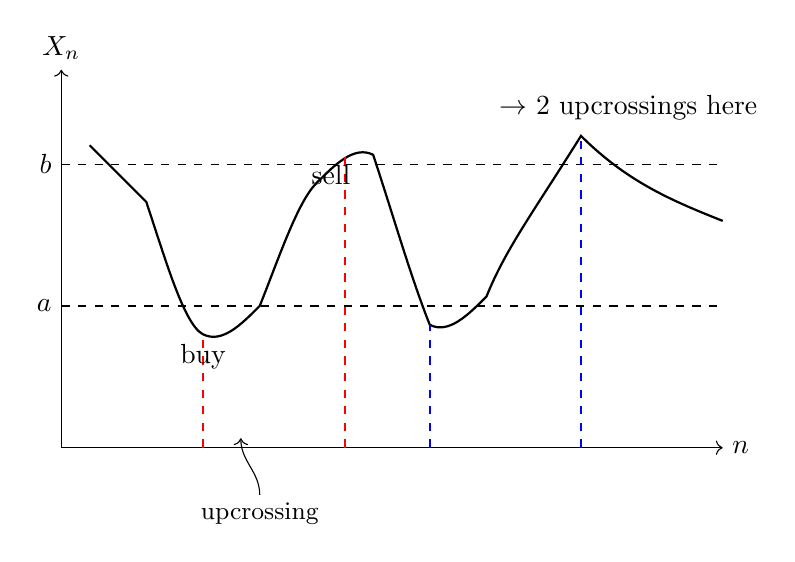
\begin{tikzpicture}[scale=1.2]
% Draw axes
\draw[->] (0,0) -- (7,0) node[right] {$n$};
\draw[->] (0,0) -- (0,4) node[above] {$X_n$};

% Draw the horizontal lines for a and b
\draw[dashed] (0,1.5) -- (7,1.5);
\draw[dashed] (0,3) -- (7,3);
\node[left] at (0,1.5) {$a$};
\node[left] at (0,3) {$b$};

% Draw a sample path with upcrossings (generally decreasing for supermartingale)
\draw[thick] (0.3,3.2) 
    .. controls (0.5,3.0) and (0.7,2.8) .. (0.9,2.6)
    .. controls (1.1,2.0) and (1.3,1.3) .. (1.5,1.2)
    .. controls (1.7,1.1) and (1.9,1.3) .. (2.1,1.5)
    .. controls (2.3,2.0) and (2.5,2.6) .. (2.7,2.8)
    .. controls (2.9,3.0) and (3.1,3.2) .. (3.3,3.1)
    .. controls (3.5,2.5) and (3.7,1.8) .. (3.9,1.3)
    .. controls (4.1,1.2) and (4.3,1.4) .. (4.5,1.6)
    .. controls (4.7,2.1) and (5.0,2.5) .. (5.5,3.3)
    .. controls (6.0,2.8) and (6.5,2.6) .. (7,2.4);

% Mark the upcrossings with vertical dashed lines
\draw[dashed, thick, red] (1.5,0) -- (1.5,1.2) node[below, black] {buy};
\draw[dashed, thick, red] (3,0) -- (3,3.1) node[below, black, xshift=-5pt] {sell};
\draw[dashed, thick, blue] (3.9,0) -- (3.9,1.3);
\draw[dashed, thick, blue] (5.5,0) -- (5.5,3.3);

% Add annotations
\node at (2.1,-0.7) {\small upcrossing};
\draw[->] (2.1,-0.5) to[out=90,in=-90] (1.9,0.1);

\node at (6,3.6) {$\rightarrow$ 2 upcrossings here};
\end{tikzpicture}
\end{center}

\begin{theorem}[Doob's Upcrossing Inequality for Supermartingales]
For a supermartingale $(X_n)$ and constants $a < b$,
\[
(b-a) \mathbb{E}[U_N([a,b])] \leq \mathbb{E}[(X_N - a)^-]
\]
where $(x)^- = \max(-x, 0)$ denotes the negative part.
\end{theorem}
\noindent Consider a trading strategy where we buy the supermartingale when it drops below $a$ and sell when it rises above $b$. Each complete upcrossing generates a profit of at least $b - a$. The total expected profit from all upcrossings is therefore at least $(b-a)\mathbb{E}[U_N([a,b])]$. However, for a supermartingale, the expected value tends to decrease over time. The total profit from this strategy is bounded by how far the process can drop below $a$ by time $N$, which is captured by $(X_N - a)^-$. 


\begin{itemize}
\item For submartingales: $(b-a) \mathbb{E}[U_N([a,b])] \leq \mathbb{E}[(X_N - a)^+]$ (bounded by positive part)
\item For supermartingales: $(b-a) \mathbb{E}[U_N([a,b])] \leq \mathbb{E}[(X_N - a)^-]$ (bounded by negative part)
\item The inequality for submartingales follows by applying the supermartingale inequality to $-X_n$
\end{itemize}
\noindent We now formally prove Doob's Upcrossing Inequality
\begin{proof}
Define a trading strategy $C_n$ which buys when the process is below $a$ and sells when above $b$. The cumulative gain from trading is
\[
Y_n = \sum_{k=1}^n C_k (X_k - X_{k-1})
\]
Since $C$ is predictable and non-negative, and $X$ is a supermartingale, $Y$ is also a supermartingale with $Y_0 = 0$. The key observation is that
\[
(b-a) U_N([a,b]) \leq Y_N + (X_N - a)^-
\]
(where $(X_N - a)^-$ is the penalty term that accounts for an incomplete final upcrossing). Taking expectations and using the supermartingale property gives the result.
\end{proof}
\noindent If $X$ is bounded in $L^1$ (that is $\sup \limits _n \mathbb{E}(|X_n|) < \infty$, then we have that \[
\mathbb{E}((X_n - a)^-) \le \mathbb{E}(|X_n|) + |a|
\]
So \[
\sup \limits _{N} \mathbb{E} (U_N([a,b])) \le \frac{1}{b-a} \sup _N (\mathbb{E}(|X_n|) + |a|) < \infty
\]
So by defining $U_\infty ([a,b]) = \lim \limits _{N \to \infty }U_N([a,b])$, (whose limit exists because $U_N([a,b])$ is an increasing sequence and bounded above) and using Monotone Convergence, we get
\[
\mathbb{E}[U_\infty([a,b])] < \infty
\]
But then the integral \[
\int _\Omega |X_n| d\mathbb{P}
\]
is finite which implies $U_\infty ([a,b])$ is finite almost surely. This proves that the supermartingale can have only finitely many oscillations between $a$ and $b$, establishing that $X_n$ must converge almost surely and so $\mathbb{P}(U_{\infty} [a,b] = \infty) = 0$. Combined with the submartingale version, this forms the foundation of Doob's Martingale Convergence Theorem for general supermartingales and submartingales (it is used in the proof below)



\subsection{Doob's Convergence Theorem}

\begin{theorem}[Doob's Convergence Theorem]\label{thm:doob_convergence}
If $(X_n)$ is a supermartingale (or submartingale or martingale) bounded in $L^1$ (equivalently, the upcrossings are finite), i.e., $\sup_n \mathbb{E}[|X_n|] < \infty$, then $X_n$ converges almost surely to some finite RV $X_\infty$. That is, \[
X_n \xrightarrow{a.s.}X_\infty \text{ as } n \to \infty
\]
\end{theorem}

\begin{proof}
    Let $A = \{\omega \in \Omega: X_n (\omega) \text{ does not converge}\}$. We must show $A$ is a null set. We have that \begin{align*}
        A & = \{\omega \in \Omega: \liminf \limits _{n \to \infty} X_n (\omega) < \limsup \limits _{n \to \infty} X_n (\omega)\} \\ & = \bigcup \limits _{\substack{a,b \in \mathbb{Q}\\ a < b} } \{ \omega \in \Omega : \liminf \limits _{n \to \infty} X_n(\omega) < a <b<\limsup \limits _{n \to \infty} X_n (\omega)\} \\ & = \bigcup \limits _{\substack{a,b \in \mathbb{Q}\\ a < b} } \{\omega \in \Omega: U_{\infty} ([a,b]) = \infty\}
    \end{align*}
    which is a null set since $X_n \in L^1$
\end{proof}

\begin{corollary}
If $(X_n)$ is a supermartingale (or submartingale or martingale) bounded in $L^p$, i.e., $\sup_n \mathbb{E}[|X_n|^p] < \infty$, then $X_n$ converges almost surely to some finite RV $X_\infty$. That is, \[
X_n \xrightarrow{a.s.}X_\infty \text{ as } n \to \infty
\]
\end{corollary}

\begin{proof}
By Jensen's Inequality, \[
\mathbb{E}(|X_n|) \le (\mathbb{E}(|X_n|^p))^{1/p}
\]
So bounded in $L^p$ implies bounded in $L^1$, then use Doob's Convergence Theorem.
\end{proof}

\begin{theorem}[UI Sub/Supermartingale Convergence Theorem]
Let $(X_n)$ be a submartingale with respect to a filtration $(\mathcal{F}_n)$. The following are equivalent:
\begin{enumerate}
    \item $(X_n)$ is uniformly integrable.
    
    \item $(X_n)$ converges almost surely and in $L^1$ to some random variable $X_\infty$.
    
    \item $(X_n)$ converges in $L^1$ to some random variable $X_\infty$.
\end{enumerate}
Moreover, if $(X_n)$ is UI, then $X_\infty \in L^1$ and
\[
X_n \leq \mathbb{E}[X_\infty \mid \mathcal{F}_n] \quad \text{for all } n \in \mathbb{N}.
\]
(and $\ge$ for a supermartingale)
\end{theorem}

\begin{proof}
~\\ $(1) \Longrightarrow (2)$: ~\\
    We know $X_n \to X_\infty$ a.s. since $X$ being UI means it is in $L^1$ (Theorem~\ref{thm:ui-L}) and thus, by Doob's Convergence Theorem (Theorem~\ref{thm:doob_convergence}), it converges almost surely to some $X_\infty$. But then by Vitali's Theorem (Theorem~\ref{thm:vitali}), $X_n \to X_\infty$ in $L^1$
    ~\\~\\ $(2) \Longrightarrow (1)$ ~\\
    Convergence in $L^1$ implies $X_n, X_\infty \in L^1$, so by Vitali's Theorem, $(X_n)$ is UI.
    ~\\~\\ $(2) \Longrightarrow (3)$ ~\\
    Trivial
    ~\\~\\ $(3) \Longrightarrow (1)$ ~\\
    Convergence in $L^1$ implies $X_n, X_\infty \in L^1$, so by Vitali's Theorem, $(X_n)$ is UI.
    ~\\~\\ Now if $(X_n)$ is UI, we have shown $X_\infty \in L^1$. We have that \[
    X_n \le \mathbb{E}(X_m | \mathcal{F}_n)
    \] for $m > n$. By the Partial Averaging Property, for any $A \in \mathcal{F}_n$, \[
    \int _A X_n d\mathbb{P} \le \int _A \mathbb{E}(X_m | \mathcal{F}_n)d\mathbb{P} = \int _A X_m d\mathbb{P}
    \]
    But now we claim that $\lim \limits _{m \to \infty} \int _A X_m d\mathbb{P} = \int _A X_\infty d\mathbb{P}$. We have that \[
    \left | \int _A X_m d\mathbb{P} -  \int _A X_\infty d\mathbb{P}  \right | = \left | \int _A X_m - X_\infty d\mathbb{P} \right | \le \int _A |X_m - X_\infty |d\mathbb{P} \le \int _\Omega |X_m - X_\infty |d\mathbb{P} \to 0
    \]
    So we have shown that \[
    \int _A X_n d\mathbb{P} \le \int _A X_\infty d\mathbb{P} = \int _A \mathbb{E} (X_\infty |\mathcal{F}_n) d\mathbb{P}
    \]
    But this implies $X_n \le \mathbb{E} (X_\infty | \mathcal{F}_n )$ $\mathbb{P}$-a.e.
\end{proof}
\begin{theorem}[UI Martingale Convergence Theorem]
Let $(X_n)$ be a martingale with respect to a filtration $(\mathcal{F}_n)$. The following are equivalent:
\begin{enumerate}
    \item $(X_n)$ is uniformly integrable.
    
    \item $(X_n)$ converges almost surely and in $L^1$ to some random variable $X_\infty$.
    
    \item $(X_n)$ converges in $L^1$ to some random variable $X_\infty$.
    
    \item There exists a random variable $X_\infty \in L^1(\mathcal{F}_\infty)$ such that
    \[
    X_n = \mathbb{E}[X_\infty \mid \mathcal{F}_n] \quad \text{for all } n \in \mathbb{N},
    \]
    where $\mathcal{F}_\infty = \sigma\left(\bigcup_{n=1}^\infty \mathcal{F}_n\right)$.
\end{enumerate}
When these conditions hold, we say the martingale is \textbf{closed} by $X_\infty$.
\end{theorem}

\begin{proof}
    A martingale is a submartingale which shows $(1) \iff (2) \iff (3)$. By proceeding as above, we obtain equality (with martingale) so $(1) \Longrightarrow (4)$. The reverse direction is in the tutorial
\end{proof}

\begin{remark}
The fourth condition is unique to martingales. It characterizes UI martingales as precisely those that can be represented as conditional expectations of an $L^1$ random variable. This is sometimes called a \textbf{Doob martingale} or a \textbf{regular martingale}.
\end{remark}


\subsection{Square Integrable Martingales}

\begin{definition}[Square--integrable martingale]
Let $(M_t)$ be a martingale with respect to filtration $(\mathcal{F}_t)_{t\in T}$ be a martingale (where $T=\mathbb{N}$ 
or $T=[0,\infty)$).  
We say that $M$ is \emph{square integrable} if
\[
M_t \in L^2 \qquad \text{for all } t\in T \iff \mathbb{E}(M_t^2) < \infty, \quad \text{ for all } t \in T
\]
We say that $M$ is \emph{bounded in $L^2$} if
\[
\sup_{t\in T} \mathbb{E}[M_t^2] < \infty.
\]
\end{definition}

\begin{remark}
Every bounded-in-$L^2$ martingale is square integrable, but not conversely.
\end{remark}

\begin{theorem}[Properties of square--integrable martingales]
Let $(M_t)$ be a square--integrable martingale.
\begin{enumerate}

\item[\textnormal{(1)}] \textbf{$L^2$--orthogonality of increments  
(discrete time only).}  
If $T=\mathbb{N}$, then for integers $0 \le m<n<k<\ell$,
\[
\mathbb{E}\big[(M_n-M_m)(M_\ell-M_k)\big]=0.
\]

\item[\textnormal{(2)}] \textbf{Energy identity (discrete time only).}  
If $T=\mathbb{N}$$, then$
\[
M_n = M_0 + \sum_{k=1}^n (M_k - M_{k-1}),
\]
and the increments are orthogonal in $L^2$, giving
\[
\mathbb{E}[M_n^2]
= \mathbb{E}[M_0^2] + \sum_{k=1}^n \mathbb{E}\big[(M_k-M_{k-1})^2\big].
\]


\item[\textnormal{(3)}] \textbf{Martingale convergence in $L^2$  
(bounded-in-$L^2$ case).}  
If $\sup_t \mathbb{E}[M_t^2] < \infty$ (discrete or continuous time),
then there exists $M_\infty \in L^2$ such that
\[
M_t \longrightarrow M_\infty \quad \text{in } L^2 \text{ and a.s.}
\]

\item[\textnormal{(4)}] \textbf{Hilbert space structure (bounded-in-$L^2$).}  
Let $H$ be the space
\[
H := \{ M : M \text{ is a martingale and } \sup_t \mathbb{E}[M_t^2]<\infty\}.
\]
Define
\[
\langle M,N\rangle := \mathbb{E}[M_\infty N_\infty].
\]
Then $(H,\langle\cdot,\cdot\rangle)$ is a Hilbert space.
Here $M_\infty$ is the $L^2$ limit guaranteed by (3).

\end{enumerate}
\end{theorem}

\begin{proof}
\textbf{(1) Orthogonality of increments.}
Fix $0\le u < n < t < s$. Then
\[
\mathbb{E}\big[(M_n - M_u)(M_s - M_t)\big]
    = \mathbb{E}\big[ (M_n - M_u)\,
       \mathbb{E}(M_s - M_t \mid \mathcal{F}_t) \big],
\]
by the tower property and the fact that $M_n - M_u$ is
$\mathcal{F}_t$–measurable.
Since $(M_n)$ is a martingale,
\[
\mathbb{E}(M_s - M_t \mid \mathcal{F}_t)
    = \mathbb{E}(M_s \mid \mathcal{F}_t) - M_t = M_t - M_t = 0.
\]
Hence the inner conditional expectation is zero, and thus
\[
\mathbb{E}\big[(M_n - M_u)(M_s - M_t)\big] = 0,
\]
so increments over disjoint intervals are $L^2$–orthogonal.

\medskip

\textbf{(2) Energy identity.}
Write $\Delta M_k := M_k - M_{k-1}$. Then
\[
M_n = M_0 + \sum_{k=1}^n \Delta M_k.
\]
By (1), the random variables $M_0,\Delta M_1,\dots,\Delta M_n$ are
pairwise orthogonal in $L^2$. Therefore
\[
\mathbb{E}[M_n^2]
 = \left\| M_0 + \sum_{k=1}^n \Delta M_k \right\|_2^2
 = \|M_0\|_2^2 + \sum_{k=1}^n \|\Delta M_k\|_2^2
 = \mathbb{E}[M_0^2] + \sum_{k=1}^n \mathbb{E}[(\Delta M_k)^2].
\]

\medskip

\textbf{(3) $L^2$ convergence when $\sup_n \mathbb{E}[M_n^2]<\infty$.}
Assume $\sup_n \mathbb{E}[M_n^2] < \infty$.
From (2) we have, for $m<n$,
\[
\mathbb{E}[(M_n - M_m)^2]
  = \mathbb{E}[M_n^2] - \mathbb{E}[M_m^2]
  = \sum_{k=m+1}^n \mathbb{E}[(\Delta M_k)^2].
\]
Taking $m\to\infty$ and using the boundedness of $\mathbb{E}[M_n^2]$,
we see that $\sum_{k=1}^\infty \mathbb{E}[(\Delta M_k)^2] < \infty$, hence
the tail sums
\[
\sum_{k=m+1}^n \mathbb{E}[(\Delta M_k)^2]
\]
tend to $0$ as $m,n\to\infty$. Thus $(M_n)$ is a Cauchy sequence in $L^2$,
so there exists $M_\infty \in L^2$ with $M_n \to M_\infty$ in $L^2$.
~\\~\\
Since $L^2$ convergence implies convergence in probability, and any
sequence that is Cauchy in $L^2$ admits an almost-surely convergent
subsequence, a standard argument shows that the whole sequence converges
to $M_\infty$ almost surely as well.

\medskip

\textbf{(4) Hilbert space structure.}
First we show that for $M\in H$ and the limit $M_\infty$ from (3),
\[
M_n = \mathbb{E}[M_\infty \mid \mathcal{F}_n] \quad \text{a.s. for all } n.
\]
Indeed, for any $m>n$,
\[
\mathbb{E}[M_m \mid \mathcal{F}_n] = M_n
\]
by the martingale property. As $m\to\infty$, we have
$M_m \to M_\infty$ in $L^2$, and conditional expectation is a
continuous linear operator on $L^2$ with norm $1$, so
\[
\mathbb{E}[M_m \mid \mathcal{F}_n] \to \mathbb{E}[M_\infty \mid \mathcal{F}_n]
\quad \text{in } L^2.
\]
Hence $M_n = \mathbb{E}[M_\infty \mid \mathcal{F}_n]$ a.s.

Now define for $M,N \in H$
\[
\langle M,N \rangle_H := \mathbb{E}[M_\infty N_\infty].
\]
Symmetry and bilinearity are immediately obvious. For positive definiteness, note that
$\langle M,M\rangle_H = 0$ implies $M_\infty = 0$ a.s., and then
$M_n = \mathbb{E}[M_\infty \mid \mathcal{F}_n] = 0$ a.s.\ for all $n$,
so $M$ is the zero martingale.

Thus $\langle\cdot,\cdot\rangle_H$ is an inner product on $H$, and
$\|M\|_H := \sqrt{\langle M,M\rangle_H} = \|M_\infty\|_{L^2}$.

To show completeness, let $(M^{(j)})_{j\ge1}$ be a Cauchy sequence in $H$.
Then the terminal variables $M^{(j)}_\infty$ form a Cauchy sequence in
$L^2$, hence converge to some $X \in L^2$. Define
\[
M_n := \mathbb{E}[X \mid \mathcal{F}_n], \qquad n\ge0.
\]
Then $(M_n)$ is a martingale with $\sup_n \mathbb{E}[M_n^2]
\le \mathbb{E}[X^2]<\infty$, so $M\in H$ and $M_\infty = X$.
By construction,
\[
\|M^{(j)} - M\|_H^2
   = \mathbb{E}\big[(M^{(j)}_\infty - X)^2\big]
   \longrightarrow 0,
\]
so $M^{(j)} \to M$ in $H$. Therefore $H$ is complete and hence is a
Hilbert space.
\end{proof}

\textcolor{red}{NOTE:} We can alternatively prove completeness using the isometry between $H$ and $L^2$, $M \mapsto M_\infty$.

\begin{theorem}
    If $(X_k)_{k=1}^\infty$ are independent RVs (not neccessarily identically distributed) such that $\mathbb{E}(X_k) = 0$, $\text{Var}(X_k) = \sigma _k^2 < \infty$, then \[
    \sum \limits _{k=1}^{\infty} \sigma _k ^2 < \infty
    \]
    implies \[
    \sum \limits _{k=1}^{\infty} X_k \ \text{ converges a.s.}
    \]
\end{theorem}

\begin{proof}
    Define $(S_n)$ by $S_0 = 0$, $S_n = \sum \limits _{k=1}^n X_k$. Then $(S_n)$ is a martingale. Then \[
    \mathbb{E}(S_n^2) = \sum \limits _{k=1}^n \sigma _k^2 \text{ by independence}
    \]
    So \[\sup \limits _{n} \mathbb{E} (S_n^2) = \sup \limits _n \sum \limits _{k=1}^n \sigma _k^2 = \sum \limits _{k=1}^\infty \sigma _k^2 < \infty\]
    So $(S_n)$ is bounded in $L^2$ and so $(S_n) \in H$ (and thus converges a.s.)
\end{proof}

\subsection{Optional Sampling Theorem}

\begin{definition}[Stopping Time]
Let $(\Omega, \mathcal{F}, (\mathcal{F}_t)_{t \geq 0}, \mathbb{P})$ be a filtered probability space. A random variable $\tau : \Omega \to \overline{\mathbb{R}}^+$ (where $\overline{\mathbb{R}}^+ = [0, \infty]$) is called a \textbf{stopping time} if
\[
\{\tau \leq t\} \in \mathcal{F}_t \quad \text{for all } t \in \overline{\mathbb{R}}^+.
\]
\end{definition}

\begin{definition}[Stopping Time $\sigma$-Algebra]
Let $(\Omega, \mathcal{F}, (\mathcal{F}_t)_{t \geq 0}, \mathbb{P})$ be a filtered probability space and $\tau : \Omega \to \overline{\mathbb{R}}^+$ be a stopping time. We define the \textbf{stopping time $\sigma$-algebra} $\mathcal{F}_\tau$ to be
\[
\mathcal{F}_\tau := \left\{ A \in \mathcal{F} : A \cap \{\tau \leq t\} \in \mathcal{F}_t \text{ for all } t \in \overline{\mathbb{R}}^+ \right\}.
\]
\end{definition}

\begin{remark}[Interpretation]
The $\sigma$-algebra $\mathcal{F}_\tau$ represents the collection of events that can be determined by time $\tau$. In other words, $\mathcal{F}_\tau$ contains all events whose occurrence or non-occurrence is known when the stopping time $\tau$ occurs.
~\\~\\
For an event $A$ to be in $\mathcal{F}_\tau$, we require that for every fixed time $t$, the restriction of $A$ to the event $\{\tau \leq t\}$ (i.e., when the stopping has occurred by time $t$) must be measurable with respect to the information available at time $t$, namely $\mathcal{F}_t$.
\end{remark}

\begin{remark}[Special Case]
If $\tau \equiv t$ is a constant stopping time (always equal to some fixed time $t \geq 0$), then
\[
\mathcal{F}_\tau = \mathcal{F}_t.
\]
This shows that the definition generalizes the notion of the $\sigma$-algebra at a fixed time to random times.
\end{remark}

\begin{proof}[Proof of Remark]
    Let $A \in \mathcal{F}_\tau$. Then \[
    A \cap \underbrace{\{\tau \le t\}}_{= \Omega} \in \mathcal{F}_t \Longrightarrow A \in \mathcal{F}_t
    \]
    Now let $A \in \mathcal{F}_t$. We have that \[
    A \cap \{\tau \le s\} = \begin{cases}
        \emptyset  & \text{if } s <t \\ A \cap \Omega & \text{otherwise}
    \end{cases} \in \mathcal{F}_s
    \]
\end{proof}

\begin{theorem}
    We have the following properties:
    \begin{enumerate}
    \item $\mathcal{F}_\tau$ is indeed a $\sigma$-algebra.
    
    \item The stopping time $\tau$ itself is $\mathcal{F}_\tau$-measurable.
    
    \item If $\sigma$ and $\tau$ are stopping times with $\sigma \leq \tau$ almost surely, then $\mathcal{F}_\sigma \subseteq \mathcal{F}_\tau$.
    
    
    \item Assume $\mathbb{I} \subseteq \mathbb{N}$. Then \[
    \mathcal{F}_\tau =  \{A \in \mathcal{F} : A \cap \{\tau = n\} \in \mathcal{F}_n, \forall n\}
    \]
    \item If $\mathbb{I} \subseteq \mathbb{N}$ and $X$ is adapted, and $\tau$ a stopping time, then $\tau$ and $X_\tau$ are both $\mathcal{F}_\tau$-measurable.
\end{enumerate}
\end{theorem}

\begin{proof} $ $ 
    \begin{enumerate}
        \item We check the three defining properties.

(i) $\Omega\in\mathcal{F}_\tau$:
for any $t$,
\[
\Omega\cap\{\tau\le t\} = \{\tau\le t\}\in\mathcal{F}_t
\]
because $\tau$ is a stopping time. Hence $\Omega\in\mathcal{F}_\tau$.

(ii) Closed under complements: let $A\in\mathcal{F}_\tau$. Then for any $t$,
\[
A^c \cap \{\tau\le t\}
= \{\tau\le t\}\setminus (A\cap\{\tau\le t\}),
\]
and both $\{\tau\le t\}$ and $A\cap\{\tau\le t\}$ belong to $\mathcal{F}_t$,
so their difference is in $\mathcal{F}_t$. Thus $A^c\in\mathcal{F}_\tau$.

(iii) Closed under countable unions: let $(A_k)_{k\ge1}\subset\mathcal{F}_\tau$.
For each $t$,
\[
\Big( \bigcup_{k=1}^\infty A_k \Big)\cap\{\tau\le t\}
= \bigcup_{k=1}^\infty \big(A_k\cap\{\tau\le t\}\big),
\]
a countable union of sets in $\mathcal{F}_t$, hence in $\mathcal{F}_t$.
Therefore $\bigcup_k A_k\in\mathcal{F}_\tau$.

So $\mathcal{F}_\tau$ is a $\sigma$--algebra.
        \item Let $A \in \mathcal{F}_\sigma $ and $t \in \mathbb{I}$. We have that \[
        A \cap \{\tau \le t\} = \underbrace{A \cap \{\sigma \le t\}}_{\in \mathcal{F}_t \ (A \in \mathcal{F}_\sigma)  } \cap \underbrace{\{\tau \le t\}}_{_{\in \mathcal{F}_t } \text{ (stop time)}} \in \mathcal{F}_t
        \]
        \item Let $A\in\mathcal{F}_\sigma$. We must show $A\in\mathcal{F}_\tau$, i.e.,
for every $t$,
\[
A\cap\{\tau\le t\} \in \mathcal{F}_t.
\]
Since $\sigma\le\tau$ a.s., we have the inclusion
\(\{\tau\le t\}\subset\{\sigma\le t\}\). Then
\[
A\cap\{\tau\le t\}
= \big(A\cap\{\sigma\le t\}\big)\cap\{\tau\le t\}.
\]
By definition of $\mathcal{F}_\sigma$, $A\cap\{\sigma\le t\}\in\mathcal{F}_t$,
and also $\{\tau\le t\}\in\mathcal{F}_t$, so their intersection is in
$\mathcal{F}_t$. Hence $A\in\mathcal{F}_\tau$, and the inclusion follows.
\item Assume $I\subset\mathbb{N}$.  
Define
\[
\mathcal{G}_\tau := \big\{ A\in\mathcal{F}:
      A\cap\{\tau=n\}\in\mathcal{F}_n \ \forall n\in I \big\}.
\]
We show $\mathcal{F}_\tau = \mathcal{G}_\tau$.

\emph{First inclusion: $\mathcal{F}_\tau \subset \mathcal{G}_\tau$.}
Let $A\in\mathcal{F}_\tau$. Fix $n\in I$. Then
\[
A\cap\{\tau=n\}
= A\cap\{\tau\le n\}\cap\{\tau\ge n\}.
\]
We have $A\cap\{\tau\le n\}\in\mathcal{F}_n$ by definition of $\mathcal{F}_\tau$.
Also
\[
\{\tau\ge n\} = \Omega\setminus\{\tau\le n-1\},
\]
and $\{\tau\le n-1\}\in\mathcal{F}_{n-1}\subset\mathcal{F}_n$, so
$\{\tau\ge n\}\in\mathcal{F}_n$. Hence
$A\cap\{\tau=n\}\in\mathcal{F}_n$, so $A\in\mathcal{G}_\tau$.

\emph{Second inclusion: $\mathcal{G}_\tau \subset \mathcal{F}_\tau$.}
Let $A\in\mathcal{G}_\tau$. Fix $n\in I$. Then
\[
\{\tau\le n\} = \bigcup_{k\le n} \{\tau=k\},
\]
so
\[
A\cap\{\tau\le n\}
= \bigcup_{k\le n} \big(A\cap\{\tau=k\}\big).
\]
By assumption, $A\cap\{\tau=k\}\in\mathcal{F}_k\subset\mathcal{F}_n$
for each $k\le n$, and $\mathcal{F}_n$ is a $\sigma$--algebra, so the union
belongs to $\mathcal{F}_n$. Thus $A\in\mathcal{F}_\tau$, proving the equality.

\item Assume $I\subset\mathbb{N}$ and $X=(X_n)_{n\in I}$ is adapted, i.e.
$X_n$ is $\mathcal{F}_n$--measurable for each $n$.
Let $B\in\mathcal{B}(\mathbb{R})$ be a Borel set and define
\[
A := \{ X_\tau \in B \} = \{\omega : X_{\tau(\omega)}(\omega)\in B\}.
\]
We need to show $A\in\mathcal{F}_\tau$, i.e.\ for each $n$,
$A\cap\{\tau=n\}\in\mathcal{F}_n$.

For fixed $n$,
\[
A\cap\{\tau=n\}
= \{\tau=n\}\cap\{ X_\tau \in B \}
= \{\tau=n\}\cap\{ X_n \in B \},
\]
because on $\{\tau=n\}$ we have $X_\tau = X_n$.
Since $X_n$ is $\mathcal{F}_n$--measurable, the event $\{X_n\in B\}$
lies in $\mathcal{F}_n$, and $\{\tau=n\}\in\mathcal{F}_n$ (stopping time),
so their intersection is in $\mathcal{F}_n$.

Thus $A\cap\{\tau=n\}\in\mathcal{F}_n$ for all $n$, and by item (4),
$A\in\mathcal{F}_\tau$. Hence $X_\tau$ is $\mathcal{F}_\tau$--measurable.
    \end{enumerate}
\end{proof}

\begin{example}[Coin Flip Process]
Let $\Omega = \{HH, HT, TH, TT\}$ represent the outcomes of flipping a fair coin twice, where $H$ represents heads and $T$ represents tails. Define:

\begin{itemize}
    \item $\mathcal{F}^0 = \{\emptyset, \Omega\}$ 
    \item $\mathcal{F} = \mathcal{P}(\Omega) $
    \item $\mathcal{F}_1 = \sigma(\{HH, HT\}, \{TH, TT\})$ (information after first flip)
    \item $\mathcal{F}_2 = \mathcal{F}$ (complete information after second flip)
\end{itemize}
\noindent
We have the filtration:
\[
\mathcal{F}_1 = \{\emptyset, \{HH, HT\}, \{TH, TT\}, \Omega\}, \quad \mathcal{F}_2 = \mathcal{F}.
\]
Define the process $(X_t)$ counting the number of heads by time $t$:
\begin{align*}
X_0(\omega) &= 0 \quad \text{for all } \omega \in \Omega \\
X_1(HH) &= X_1(HT) = 1 \\
X_1(TH) &= X_1(TT) = 0 \\
X_2(HH) &= 2 \\
X_2(HT) &= X_2(TH) = 1 \\
X_2(TT) &= 0
\end{align*}
Our filtration has the following tree structure (each node represents the $\sigma$-algebra at that time):

\begin{center}
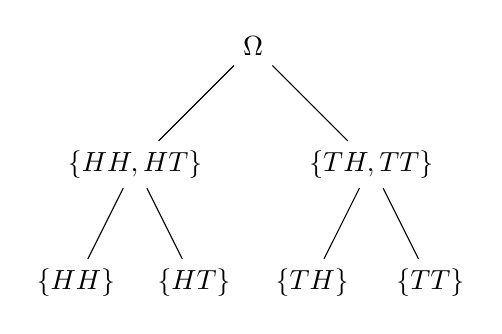
\begin{tikzpicture}[
  level distance=1.5cm,
  level 1/.style={sibling distance=3cm},
  level 2/.style={sibling distance=1.5cm}
]
\node {$\Omega$}
  child {node {$\{HH, HT\}$}
    child {node {$\{HH\}$}}
    child {node {$\{HT\}$}}
  }
  child {node {$\{TH, TT\}$}
    child {node {$\{TH\}$}}
    child {node {$\{TT\}$}}
  };
\end{tikzpicture}
\end{center}
Define the stopping time:
\[
\tau(\omega) = \inf\{t : X_t(\omega) = 1\}
\]
with the convention that $\inf \emptyset = \infty$. ~\\~\\
\noindent 
This gives:
\[
\begin{array}{c|c}
\omega & \tau(\omega) \\
\hline
HH & 1 \\
HT & 1 \\
TH & 2 \\
TT & \infty
\end{array}
\]

\textbf{Computing $\mathcal{F}_\tau$}
\noindent
We need to find all events $A \in \mathcal{F}$ such that $A \cap \{\tau \leq t\} \in \mathcal{F}_t$ for all $t \geq 0$.
~\\~\\ \noindent
For $t = 1$, $\{\tau \le 1\} = \{HH, HT\}$. In $\mathcal{F}_1$, we cannot distinguish between $\{HH, HT\}$ and between $\{TH, TT\}$.  So for $A \cap \{\tau \le 1\} \in \mathcal{F}_1$, we need $\{HH, HT\} \subseteq A$ or their intersection to be empty. Since $\mathcal{F}_2$ is the full sigma algebra, this is our only condition so \[
\mathcal{F}_\tau = \{\emptyset, \{TH\}, \{TT\}, \{HH, HT\}, \{HH, HT, TT\}, \{HH, HT, TH\}, \{TT, TH\}, \Omega\}
\]
(generated by blocks $\{TT\}, \{TH\}. \{HH, HT\}$)
\end{example}

\begin{remark}
The key insight is that $\{HH\} \notin \mathcal{F}_\tau$ because at time $t = 1$ (when $\tau = 1$ for both $HH$ and $HT$), we cannot distinguish between these two outcomes using only $\mathcal{F}_1$. The second coin flip hasn't been revealed yet, so we only know the first flip was heads, not whether the second was heads or tails.
\end{remark}


\begin{theorem}[Optional Sampling Theorem]\label{thm:optional_sampling}
If $X$ is a uniformly integrable martingale and $\sigma \leq \tau$ are finite a.s. stopping times, then
\[
\mathbb{E}[X_\tau | \mathcal{F}_\sigma] = X_\sigma \text{ (a.s.)}
\]
\end{theorem}

\begin{proof}
We want to show that for all $A \in \mathcal{F}_\sigma$,
\[
\int_A X_\tau \, d\mathbb{P} \stackrel{?}{=} \int_A X_\sigma \, d\mathbb{P}.
\]
\textbf{Step 1: Partition by Stopping Time Values}
\\ ~\\ \noindent
Write $A$ as a disjoint union:
\[
A = \bigcup_{n=0}^\infty A_n, \quad \text{where } A_n = A \cap \{\sigma = n\}.
\]
Then:
\[
\int_A X_\tau \, d\mathbb{P} = \int_{\bigcup_{n=0}^\infty A_n} X_\tau \, d\mathbb{P} = \sum_{n=0}^\infty \int_{A_n} X_\tau \, d\mathbb{P}.
\]
\textbf{Step 2: Restrict to Each Stopping Time Level}
~\\~\\ \noindent
Note that on $A_n = A \cap \{\sigma = n\}$:
\begin{itemize}
    \item $X_\tau = X_n$ on $\{\tau = n\}$
    \item $X_\tau = X_m$ on $\{\tau = m\}$ for $m > n$
\end{itemize}

Since $\sigma \leq \tau$, on the set $\{\sigma = n\}$, we have $\{\tau \geq n\}$. Therefore:
\[
\int_{A_n} X_\tau \, d\mathbb{P} = \sum_{m=n}^\infty \int_{A_n \cap \{\tau = m\}} X_\tau \, d\mathbb{P}.
\]

Since $X_\tau = X_m$ on $\{\tau = m\}$:
\[
= \sum_{m=n}^\infty \int_{A_n \cap \{\tau = m\}} X_m \, d\mathbb{P}.
\]
\noindent
\textbf{Step 3: Apply the Martingale Property}
~\\~\\ \noindent
For $m \geq n$, since $A_n \in \mathcal{F}_n$ (as $A_n = A \cap \{\sigma = n\}$ where $A \in \mathcal{F}_\sigma$ and $\{\sigma = n\} \in \mathcal{F}_n$), and $\{\tau = m\} \in \mathcal{F}_m$, we have $A_n \cap \{\tau = m\} \in \mathcal{F}_m$ (in fact, $A_n \cap \{\tau = m\} \in \mathcal{F}_n$ when $m = n$). By the martingale property, for $m > n$:
\[
\mathbb{E}[X_m \mid \mathcal{F}_n] = X_n.
\]
Therefore:
\[
\int_{A_n \cap \{\tau = m\}} X_m \, d\mathbb{P} = \int_{A_n \cap \{\tau = m\}} \mathbb{E}[X_m \mid \mathcal{F}_n] \, d\mathbb{P} = \int_{A_n \cap \{\tau = m\}} X_n \, d\mathbb{P}.
\]
\textbf{Step 4: Sum Over All $m \geq n$}
~\\~\\ \noindent
\[
\int_{A_n} X_\tau \, d\mathbb{P} = \sum_{m=n}^\infty \int_{A_n \cap \{\tau = m\}} X_n \, d\mathbb{P}.
\]
Factor out $X_n$ (which is constant on each $A_n \cap \{\tau = m\}$):
\[
= \int_{A_n} X_n \, d\mathbb{P} \sum_{m=n}^\infty \mathbf{1}_{A_n \cap \{\tau = m\}}.
\]
Since $\bigcup_{m=n}^\infty \{A_n \cap \{\tau = m\}\} = A_n$ (disjoint union):
\[
= \int_{A_n} X_n \, d\mathbb{P}.
\]
But $X_n = X_\sigma$ on $A_n = A \cap \{\sigma = n\}$, so:
\[
= \int_{A_n} X_\sigma \, d\mathbb{P}.
\]
\textbf{Step 5: Sum Over All $n$}
~\\~\\ \noindent
\[
\int_A X_\tau \, d\mathbb{P} = \sum_{n=0}^\infty \int_{A_n} X_\tau \, d\mathbb{P} = \sum_{n=0}^\infty \int_{A_n} X_\sigma \, d\mathbb{P} = \int_{\bigcup_n A_n} X_\sigma \, d\mathbb{P} = \int_A X_\sigma \, d\mathbb{P}.
\]
This holds for all $A \in \mathcal{F}_\sigma$, so by the definition of conditional expectation:
\[
\mathbb{E}[X_\tau \mid \mathcal{F}_\sigma] = X_\sigma.
\]
\end{proof}

\begin{theorem}
If $X$ is a non-negative submartingale and $\tau \le \sigma$ are bounded stopping times, then \[
X_\tau \le \mathbb{E}(X_\sigma | \mathcal{F}_\tau)
\]
\end{theorem}


\subsection{Continuous-Time Stochastic Processes}

\begin{definition}[Equivalent Stochastic Processes]\label{def:equiv_processes}
Let $X = \{X_t : t \geq 0\}$ and $Y = \{Y_t : t \geq 0\}$ be stochastic processes. We say that $X$ and $Y$:
\begin{enumerate}
    \item Have the same finite dimensional distributions (f.d.d) if for all $n$, $t_1, \ldots, t_n$, and $B_1, \ldots, B_n \in \mathcal{B}(\mathbb{R})$:
    \[
    \mathbb{P}(X_{t_1} \in B_1, \ldots, X_{t_n} \in B_n) = \mathbb{P}(Y_{t_1} \in B_1, \ldots, Y_{t_n} \in B_n)
    \]
    (notation $X \stackrel{d}{=}Y$). The intuition is that any finite dimensions have the same distributions (e.g., $X_t = Y_t, (X_t, X_s) = (Y_t, Y_s)$)
    
    \item Are modifications of one another if $\forall t \geq 0: \mathbb{P}(X_t = Y_t) = 1$
    
    \item Are indistinguishable if $\mathbb{P}(\{X_t = Y_t \text{ for all } t\}) = 1$
\end{enumerate}
\end{definition}
\noindent
We have the implications: Indistinguishable $\Rightarrow$ Modifications $\Rightarrow$ Same f.d.d.

\begin{example}
    Let $T: \Omega \to \mathbb{R}$ be an $\exp (1)$ RV. Define \begin{align*}
        X_t (\omega) & = \begin{cases}
            1 & \text{if } t = T(\omega) \\ 0 & \text{otherwise}
        \end{cases} \\ Y_t(\omega) & = 0, \quad \forall t,\omega
    \end{align*}
    Fix $t \ge 0$. Then \begin{align*}
        \mathbb{P} (\{\omega \in \Omega : X_t(\omega ) = Y_t(\omega)\}) & = \mathbb{P} (\{\omega \in \Omega: X_t(\omega) = 0\}) \\ & = \mathbb{P} (\{\omega \in \Omega:T(\omega )\ne t\}) \\ & =1
    \end{align*}
    Since $T$ is a continuous RV. So $X$ is a modification of $Y$. But \[
    \mathbb{P} (\{\omega \in \Omega : X_t(\omega ) = Y_t(\omega), \forall t\}) = \mathbb{P}(\emptyset) = 0
    \]
    since none of the sample paths coincide.
\end{example}

\begin{theorem}[Regularity Theorem]\label{thm:regularity}
If $X$ and $Y$ are both left and right continuous, then $X$ is a modification of $Y$ if and only if $X$ and $Y$ are indistinguishable.
\end{theorem}

\begin{proof}
$(\Rightarrow)$ \[
\mathbb{P}(\{X_t = Y_t, \quad t \ge 0\}) = \mathbb{P}(\{X_t = Y_y \quad \forall q \in \mathbb{Q}^+\}) = \mathbb{P} \left (\bigcap_{q \in \mathbb{Q}^+} \{X_t = Y_t\}\right ) = 1
\]
(reasoning: two continuous functions agreeing on a dense subset agree everywhere, then we use the complement and $\sigma$-subadditivity)
\end{proof}

\begin{definition}
We say $X$ is measurable if it is measurable as a function \[
X: [0, \infty) \times \Omega \to \mathbb{R}
\]
with respect to $\mathcal{B}([0, \infty)) \otimes \mathcal{F}$
\end{definition}

\begin{definition}
We say $X$ is progressively measuralbe if \[
\forall t > 0: X:[0,t] \times \Omega \to \mathbb{R}
\]
\[
(t, \omega \mapsto X_t(\omega))
\]
is $\mathcal{B}([0,t]) \otimes \mathcal{F}_t$ measurable
\end{definition}

\begin{definition}
We define the predictable or previsible $\sigma$-algebra on $[0, \infty) \times \Omega$ as: \[
\mathcal{P} = \sigma (\{X:X \text{ is left continuous and adapted}\})
\]
We say $X$ is previsible if $X \in m\mathcal{P}$
\end{definition}

\begin{definition}
We define the optional $\sigma$-algebra on $[0, \infty) \times \Omega$ \[
\mathcal{O} = \sigma (\{X:X\text{ is right continuous and adapted}\})
\]
We say that $X$ is optional if $X \in m\mathcal{O}$
\end{definition}

\begin{definition}[Filtrations]
A filtration $\mathbb{F} = \{\mathcal{F}_t:t\ge 0\}$ is 
\begin{enumerate}
    \item Right continuous iff \[
        \mathcal{F}_{t^+} = \bigcap \limits _{s > t} \mathcal{F}_s = \mathcal{F}_t
    \]
    \item Complete iff $\mathcal{F}_0$ contains all the $\mathbb{P}$-null sets.
\end{enumerate}
We say that $\mathbb{F}$ satisfies the ``usual'' conditions iff $\mathcal{F}$ is right continuous and complete (proof in Rogers and Williams)
\end{definition}

\subsection{Class D Processes}

\begin{definition}[Class D]\label{def:class_d}
A stochastic process $X = \{X_t : t \geq 0\}$ is of class D if
\[
\{X_\tau : \tau \text{ is a finite stopping time}\}
\]
is uniformly integrable.

$X$ is of class DL if for all $t \geq 0$:
\[
\{X_\tau : \tau \leq t \text{ is a finite stopping time}\}
\]
is uniformly integrable.
\end{definition}


\begin{theorem}
A non-negative submartingale is of class DL.
\end{theorem}

\begin{proof}
For a bounded stopping time $\tau \le T$, we have that \[
X_\tau \le \mathbb{E}(X_T | \mathcal{F}_\tau)
\]
But the family $\{\mathbb{E}(X_T | \mathcal{F}_\tau)\}$ is uniformly integrable, so $X$ is of class DL.
\end{proof}


\begin{example}[Every martingale is of class DL]
Let $(X_t)_{t\ge0}$ be a martingale and let $a>0$.
Suppose $\tau$ is a stopping time satisfying $\tau \le a$ almost surely. By Jensen's Inequality, $|X|$ is a submartingale and is nonnegative, so it is on class DL. So \[
\{|X|_\tau : \tau \le t \text{ is a finite stopping time}\}
\]
is UI, and thus so is 
\[
\{X_\tau : \tau \le t \text{ is a finite stopping time}\}
\]
\end{example}

\begin{definition}[Local Martingale]
Let $(\Omega, \mathcal{F}, P)$ be a probability space; let 
$\mathbb{F}_* = (\mathcal{F}_t)_{t \ge 0}$ be a filtration of $\mathcal{F}$; 
and let 
\[
X : [0,\infty) \times \Omega \to S
\]
be an $\mathbb{F}_*$-adapted stochastic process with values in a set $S$.
We say that $X$ is an \emph{$\mathbb{F}_*$-local martingale} if there exists
a sequence of $\mathbb{F}_*$-stopping times
\[
\tau_k : \Omega \to [0,\infty), \qquad k \in \mathbb{N},
\]
such that:
\begin{enumerate}
    \item The sequence $(\tau_k)$ is almost surely increasing:
    \[
    P\{\tau_k < \tau_{k+1}\} = 1;
    \]
    \item The stopping times diverge almost surely:
    \[
    P\!\left( \lim_{k \to \infty} \tau_k = \infty \right) = 1;
    \]
    \item For each $k$, the stopped process
    \[
    X^{\tau_k}_t := X_{\min\{t,\tau_k\}}
    \]
    is an $\mathbb{F}_*$-martingale.
\end{enumerate}
\end{definition}

~\\~\\
\begin{theorem}
A local martingale is a martingale if and only if it is of class DL
\end{theorem}

\begin{proof}
We have just shown that if a local martingale is a martingale, it is of class DL. Now suppose a local martingale $X$ is of class DL. Since it is a local martingale, there exists an increasing sequence of stopping times $\tau_k$ such that the stopped process $X^{\tau_k}$ is a martingale. We wish to show, for $s \le t$, that \[
\mathbb{E}(X_t | \mathcal{F}_s) = X_s
\]
which is equivalent to showing for $A ]in \mathcal{F}_s$, \[
\int _A (X_t - X_s) d\mathbb{P} = 0
\]
Now, for each $k$, the stopped processes $X_{\tau_k \land t}$ and $X_{\tau_k \land s}$ are martingales. Let $T > t$. Then the set \[
\{X_\tau : \tau \le T \text{ is a finite stopping time}\}
\]
is uniformly integrable. So $\{X_{\tau_k \land t}\}$ and $\{X_{\tau_k \land s}\}$ are uniformly integrable. But $M_{t \land \tau_n} \to M_t$ and $M_{s \land \tau_n} \to M_s$ a.s., so $M_{t \land \tau_n} \to M_t$ and $M_{s \land \tau_n} \to M_s$ in $L^1$. So \[
\left |\mathbb{E}(M_{t \land \tau_n} - M_{s \land \tau_n} I_A) - \mathbb{E}((M_t - M_s)I_A) \right| \le \mathbb{E}(|M_{t \land \tau_n}|) + \mathbb{E}(|M_{s \land \tau_n} - M_s) \to 0
\]
So it follows that $\mathbb{E}((M_t - M_s)I_A) = 0$ and so $M$ is a martingale.
\end{proof}

\begin{theorem}
A martignale is of class D iff it is uniformly integrable.
\end{theorem}

\begin{proof}
Let $(X_t)_{t\ge0}$ be a uniformly integrable martingale.  Then there exists
an integrable random variable $X_\infty\in L^1$ such that
\[
X_t = \mathbb{E}(X_\infty \mid \mathcal{F}_t), \qquad t\ge0.
\]
Let $\tau$ be any finite stopping time.  We claim that 
\[
X_\tau = \mathbb{E}(X_\infty \mid \mathcal{F}_\tau).
\]
Let $A \in \mathcal{F}_\tau$. We want to show that \[
\int_A X_\tau d\mathbb{P} = \int_A X_\infty d\mathbb{P}
\]
Let $\tau_n = \tau \land n$. Then $\tau_n$ is a finite stopping time, so, by the Optional Sampling Theorem, $X_{\tau_n} = \mathbb{E}(X_n | \mathcal{F}_{\tau_n})$. So \[
\int_{A \cap \{\tau \le n\}}X_\tau d\mathbb{P} = \int_{A \cap \{\tau \le n\}}X_{\tau_n} d\mathbb{P} = \int_{A \cap \{\tau \le n\}}X_n\mathbb{P}
\]
Taking $n \to \infty$ gives us our result. Since conditional expectations of a fixed integrable random variable form a
uniformly integrable family, it follows that
\[
\{ X_\tau : \tau \text{ finite stopping time} \}
\quad\text{is uniformly integrable}.
\]
Therefore every uniformly integrable martingale is of class~D. Now if $(X_t)$ is of class D, then \[
\{X_t: t \ge 0\} \subseteq \{X_\tau : \tau \text{ is a finite stopping time}\}
\]
since the deterministic stopping time $\tau = t$ is a finite stopping time. Thus $(X_t)$ is u.i.
\end{proof}


\newpage

\section{Stochastic Integration}

\begin{theorem}[Doob's Regularity Theorem]
If $X$ is a continuous-time martingale, then it has a cadlag modification
\end{theorem}

\begin{proof}
Rogers and Williams
\end{proof}
This means we can assume every martginale is cadlag.

\subsection{Doob-Meyer Decomposition}

\begin{theorem}[Doob-Meyer Decomposition]\label{thm:doob_meyer}
Let $X$ be a submartingale of class DL. Then there exists a unique martingale $M$ and a unique predictable increasing process $A$, both null at $0$, such that
\[
X = X_0 + A + M
\]

Furthermore, $M$ is uniformly integrable if and only if $X$ is of class D.
\end{theorem}

\begin{proof}
MSC/PhD. Uses capacity theory (advanced descriptive set theory)
\end{proof}


\begin{example}[Poisson Process]\label{ex:poisson_dm}
Let $(N_t)_{t\ge 0}$ be a Poisson process of rate $\lambda>0$.  
We show that $N_t$ admits the Doob--Meyer decomposition
\[
    N_t = N_0 + M_t + A_t,
\qquad 
M_t := N_t - \lambda t,\quad
A_t := \lambda t.
\]
\textbf{(1) $N_t$ is a submartingale.}  
For $s<t$, by independent increments,
\[
N_t = N_s + (N_t - N_s),
\]
and $N_t - N_s \sim \mathrm{Poi}(\lambda(t-s))$ is independent of $\mathcal{F}_s$.  
Thus
\[
\mathbb{E}[N_t \mid \mathcal{F}_s]
    = \mathbb{E}[N_s + (N_t-N_s)\mid \mathcal{F}_s]
    = N_s + \lambda(t-s) \ge N_s.
\]
\textbf{(2) Identification of the martingale part.}  
Define
\[
M_t := N_t - \lambda t.
\]
Then
\[
\mathbb{E}[M_t \mid \mathcal{F}_s]
= \mathbb{E}[N_t - \lambda t \mid \mathcal{F}_s]
= N_s + \lambda(t-s) - \lambda t
= N_s - \lambda s
= M_s,
\]
so $(M_t)$ is a martingale.\\
\textbf{(3) Identification of the compensator.}  
Let
\[
A_t := \lambda t.
\]
The process $(A_t)$ is deterministic, continuous, increasing and therefore predictable.  
Clearly $A_0=0$.\\
\textbf{(4) Decomposition.}  
We obtain
\[
N_t = N_0 + (N_t-\lambda t) + \lambda t
    = N_0 + M_t + A_t,
\]
which is the Doob--Meyer decomposition.
\end{example}


\begin{example}[$W_t^2$ (Squared Brownian Motion)]\label{ex:bm2_dm}
Let $(W_t)_{t\ge 0}$ be a standard Brownian motion and put $X_t := W_t^2$.  
We show that
\[
    W_t^2 = X_0 + M_t + A_t,
\qquad 
M_t := W_t^2 - t,\quad 
A_t := t.
\]
\noindent
\textbf{(1) $W_t^2$ is a submartingale.}  
For $s<t$, write
\[
W_t = W_s + (W_t-W_s),
\]
where $W_t - W_s$ is independent of $\mathcal{F}_s$ and normally distributed with variance $t-s$.  
Then
\begin{align*}
\mathbb{E}[W_t^2 \mid \mathcal{F}_s]
&= \mathbb{E}[(W_s + (W_t-W_s))^2 \mid \mathcal{F}_s] \\
&= W_s^2 
  + 2W_s\mathbb{E}[W_t-W_s \mid \mathcal{F}_s]
  + \mathbb{E}[(W_t-W_s)^2] \\
&= W_s^2 + (t-s) \ge W_s^2.
\end{align*}
Hence $(W_t^2)$ is a submartingale.\\ \noindent
\textbf{(2) Identification of the martingale part.}  
Define
\[
M_t := W_t^2 - t.
\]
From the computation above,
\[
\mathbb{E}[M_t \mid \mathcal{F}_s]
= \mathbb{E}[W_t^2 - t \mid \mathcal{F}_s]
= (W_s^2 + (t-s)) - t
= W_s^2 - s
= M_s,
\]
so $(M_t)$ is a martingale.

(Equivalently, by Itô's formula,
\(
d(W_t^2)=2W_t\,dW_t + dt,
\)
and the stochastic integral is a martingale.)
\\ \noindent
\textbf{(3) Identification of the compensator.}  
Let
\[
A_t := t.
\]
Then $(A_t)$ is deterministic, continuous, increasing and hence predictable, and $A_0=0$.
~\\ \noindent
\textbf{(4) Decomposition.}  
Thus,
\[
W_t^2 = X_0 + (W_t^2 - t) + t
      = X_0 + M_t + A_t,
\]
which is the Doob--Meyer decomposition.
\end{example}


\subsection{Quadratic Variation}

\begin{definition}[Predictable Quadratic Variation]\label{def:predictable_qv}
Let $X=(X_t)_{t\ge0}$ be a square-integrable martingale.  
The \emph{predictable quadratic variation} of $X$ is the unique predictable, increasing process $\langle X\rangle$, null at $0$, such that
\[
    X_t^2 - \langle X\rangle_t
\]
is a martingale.
~\\~\\
Equivalently, since $X$ is square-integrable, the process $X^2$ is a non–negative submartingale of class $DL$.  
Hence by the Doob--Meyer decomposition, there exist a martingale $M$ and a predictable increasing process $A$, both starting at $0$, such that
\[
    X_t^2 = X_0^2 + M_t + A_t.
\]
We then define
\[
    \langle X\rangle_t := A_t,
\]
which is the compensator of the submartingale $X^2$.

\vspace{0.2cm}
\noindent
For two square-integrable martingales $X$ and $Y$, the \emph{predictable quadratic covariation} is defined as
\[
    \langle X,Y\rangle_t
    := \frac{1}{4}\Big(
            \langle X+Y\rangle_t
            - \langle X-Y\rangle_t
        \Big),
\]
which agrees with the Doob--Meyer compensator of the cross–variation process
\(
[X,Y]_t.
\)
\end{definition}

\begin{example}[Brownian Motion]\label{ex:qv_bm}
For standard Brownian motion $(W_t)$, we compute its predictable quadratic variation.

We know that
\[
    W_t^2 - t
\]
is a martingale.  
Thus by Definition~\ref{def:predictable_qv},
\[
    \langle W\rangle_t = t.
\]
\end{example}

\begin{example}[Compensated Poisson Process]\label{ex:qv_poisson}
Let $(N_t)$ be a Poisson process with rate $\lambda$.  
The compensated process
\[
    M_t := N_t - \lambda t
\]
is a square–integrable martingale.  
To compute its predictable quadratic variation, consider the submartingale $M_t^2$.

Using the fact that $N_t$ has unit jumps of size $1$, we compute:
\[
    (N_t - \lambda t)^2
        = N_t^2 - 2\lambda t\, N_t + \lambda^2 t^2.
\]
Each jump of $N$ increases $M$ by exactly $1$, so $M^2$ has jumps of size
\[
    (\Delta M_t)^2 = 1.
\]

A more conceptual approach:  
for any square–integrable martingale with jumps,
\[
    \langle M\rangle_t = \sum_{s\le t} \mathbb{E}[(\Delta M_s)^2 \mid \mathcal{F}_{s-}],
\]
and since the Poisson process has totally inaccessible jumps with predictable rate $\lambda$,
\[
    \mathbb{E}[(\Delta M_s)^2 \mid \mathcal{F}_{s-}] = 1 \cdot \lambda.
\]

Thus
\[
    \langle M\rangle_t = \lambda t.
\]

Finally,
\[
    M_t^2 - \lambda t
\]
is a martingale, which exactly matches Definition~\ref{def:predictable_qv}.

Hence the predictable quadratic variation of the compensated Poisson martingale is
\[
    \langle N - \lambda t\rangle_t = \lambda t.
\]
\end{example}


\begin{proposition}\label{prop:covariation_properties}
\begin{enumerate}
    \item $\langle X, X \rangle = \langle X \rangle$
    \item $\langle X \rangle \ge 0$ and $ = 0 \iff X = 0$? (Check this vanishing property)
    \item $\langle X, Y \rangle = \langle Y, X \rangle$
    \item Bilinear:
    \begin{enumerate}
    \item $\langle aX, Y \rangle = a \langle X, Y \rangle$
    \item $\langle X, Y+Z \rangle = \langle X, Y \rangle + \langle X, Z \rangle$
    \end{enumerate}
\end{enumerate}
\end{proposition}

We say $X$ and $Y$ (s.i.m) are strongly orthogonal if $\langle X, Y \rangle = 0$.

\begin{theorem}\label{thm:covariation_characterization}
$\langle X, Y \rangle$ is the unique finite variation, predictable process, null at zero such that $XY - \langle X, Y \rangle$ is a martingale
\end{theorem}
So $XY$ is a martingale iff $\langle X, Y \rangle = 0$.

\subsection{Stochastic Integration}

\begin{definition}[Simple Process]\label{def:simple_process}
A stochastic process $\varphi$ is simple if
\[
\varphi_t = \sum_{k=1}^{K} H_k \mathbf{1}_{(\tau_{k-1}, \tau_k]}(t)
\]
where $0 = \tau_0 < \tau_1 < \cdots < \tau_K$ are stopping times and $H_k \in b\mathcal{F}_{\tau_k}$.
~\\~\\
For a simple process $\varphi$ and square integrable martingale $M$, we define
\[
(\varphi \cdot M)_t = \sum_{k=1}^{K} H_k (M_{t \wedge \tau_k} - M_{t \wedge \tau_{k-1}})
\]
\end{definition}

\begin{theorem}\label{thm:simple_stoch_int}
If $\varphi$ is simple, then $(\varphi \cdot M) \in \mathcal{M}_2$ (the space of square integrable martingales).
\end{theorem}

\begin{definition}[Stochastic Integral Space]\label{def:l2_space}
Let $L^2(M) := \{\varphi : \varphi \text{ is predictable and } \|\varphi\|_M < \infty\}$
where
\[
\|\varphi\|_M := \left[\mathbb{E}\left(\int_0^T \varphi_t^2 d\langle M \rangle_t\right)\right]^{1/2}
\]
\end{definition}

\begin{theorem}[Stochastic Integration Isometry]\label{thm:stoch_int_isometry}
The map $I: \mathcal{S} \to \mathcal{M}_2$ given by $I(\varphi) = (\varphi \cdot M)$ is a linear isometry:
\[
\|(\varphi \cdot M)\|_{\mathcal{M}_2}^2 = \|\varphi\|_M^2
\]
\end{theorem}

\begin{theorem}\label{thm:density_simple}
$\mathcal{S}$ (simple processes) is dense in $L^2(M)$.
\end{theorem}

\begin{definition}[General Stochastic Integral]\label{def:general_stoch_int}
Let $\varphi \in L^2(M)$. We define the stochastic integral of $\varphi$ with respect to $M$ as
\[
(\varphi \cdot M) = \lim_n (\varphi_n \cdot M)
\]
for any sequence $\varphi_n \in \mathcal{S}$ such that $\varphi_n \to \varphi$ with respect to $\|\cdot\|_M$.
\end{definition}

\newpage

\section{Advanced Stochastic Calculus}

\subsection{Properties of Stochastic Integration}

\begin{theorem}[Properties of Stochastic Integrals]\label{thm:stoch_int_properties}
Let $\varphi \in L^2(X)$ where $X$ is a square integrable martingale. Then:
\begin{enumerate}
    \item \textbf{Linearity:} $\int_0^t (a\varphi_s + b\psi_s) dX_s = a\int_0^t \varphi_s dX_s + b\int_0^t \psi_s dX_s$
    
    \item \textbf{Itô Isometry:} $\mathbb{E}\left[\left(\int_0^t \varphi_s dX_s\right)^2\right] = \mathbb{E}\left[\int_0^t \varphi_s^2 d\langle X \rangle_s\right]$
    
    \item \textbf{Quadratic variation:} $\left\langle \int_0^t \varphi_s dX_s \right\rangle_t = \int_0^t \varphi_s^2 d\langle X \rangle_s$
    
    \item \textbf{Covariation:} $\left\langle \int_0^t \varphi_s dX_s, \int_0^t \psi_s dY_s \right\rangle_t = \int_0^t \varphi_s \psi_s d\langle X, Y \rangle_s$
\end{enumerate}
\end{theorem}

\subsection{Localization}

\begin{definition}[Localization]\label{def:localization}
Let $\mathcal{E}$ be a class of stochastic processes. We say that a process $X$ is locally in $\mathcal{E}$ if there exists an increasing sequence of stopping times $(T_n)$ such that $T_n \to \infty$ a.s. and $X^{T_n} \in \mathcal{E}$ for all $n$.
~\\~\\
We call $(T_n)$ a localizing sequence for $X$, and denote by $\mathcal{E}_{loc}$ the set of processes that are locally in $\mathcal{E}$.
~\\~\\
Local martingales = $\mathcal{M}_{loc}$
\end{definition}
\noindent In discrete time, the following are equivalent:
\begin{enumerate}
    \item $X$ is a local martingale
    \item $X$ is a martingale transform: $X = (\varphi \cdot M) + X_0$ for some martingale $M$
    \item $X$ is a generalized martingale: $\mathbb{E}[X_{n+1}|\mathcal{F}_n] = X_n$ without requiring $X_n \in L^1$
\end{enumerate}

\subsection{Semimartingales}

\begin{definition}[Semimartingale]\label{def:semimartingale}
A semimartingale is a process $X$ such that
\[
X = X_0 + M + A
\]
where $M \in \mathcal{M}_{loc}$ and $A$ is a process of finite variation.
~\\~\\
For a semimartingale $X$ and $\varphi \in L^2_{loc}(X)$, we define
\[
(\varphi \cdot X) = (\varphi \cdot M) + (\varphi \cdot A)
\]
\end{definition}

\begin{example}\label{ex:sde_form}
Consider the SDE form:
\[
dX_t = \mu_t dt + \sigma_t dW_t
\]
Then $X_t = X_0 + \int_0^t \mu_s ds + \int_0^t \sigma_s dW_s$ and
\[
\int_0^t \varphi_s dX_s = \int_0^t \varphi_s \sigma_s dW_s + \int_0^t \varphi_s \mu_s ds
\]
\end{example}

\subsection{Quadratic Variation for General Processes}

\begin{definition}[Quadratic Variation]\label{def:quadratic_variation}
Let $X$ be a stochastic process. We define the quadratic variation process of $X$ as
\[
[X]_t = \sup_{\Pi} \sum_{t_i \in \Pi} (X_{t_i} - X_{t_{i-1}})^2
\]
where $\Pi$ is a partition of $[0,t]$.
~\\~\\
For two stochastic processes $X$ and $Y$, we define the quadratic covariation as
\[
[X,Y]_t = \frac{1}{4}([X+Y]_t - [X-Y]_t)
\]
\end{definition}
\textbf{Key differences between $[X]$ and $\langle X\rangle$:}
\begin{itemize}
    \item $[X]$ is the \emph{quadratic variation} of a semimartingale $X$.
        It always exists for semimartingales, including Brownian motion,
        Poisson processes, jump-diffusions, etc.
    \item $\langle X\rangle$ is the \emph{predictable quadratic variation}
        (or angle bracket) of a square–integrable martingale $X$.
        It is the \emph{predictable compensator} of $[X]$.
    \item For a continuous local martingale $M$,
        \[
            [M]_t = \langle M\rangle_t,
        \]
        since the quadratic variation is already predictable.
    \item In the presence of jumps,
        \[
            [M]_t - \langle M\rangle_t
        \]
        is a purely discontinuous martingale capturing the jump contribution.
\end{itemize}


\begin{example}\label{ex:qv_examples} $ $
\begin{enumerate}
    \item For Brownian motion: $[W]_t = t = \langle W \rangle_t$
    \item For continuous locally square integrable martingales: $[X]_t = \langle X \rangle_t$
    \item For Poisson process $N$: $[N]_t = N_t$
    \item If $X$ is locally square integrable martingale: $[X] - \langle X \rangle$ is a local martingale
\end{enumerate}
\end{example}

\subsection{Itô's Formula}

\begin{theorem}[Itô's Formula]\label{thm:ito_formula}
Let $X = (X^1, \ldots, X^d)$ be a $d$-dimensional continuous semimartingale and $f: \mathbb{R}^d \to \mathbb{R}$ be a $C^2$ function.

Then $Y = f(X^1, \ldots, X^d)$ is a semimartingale and
\[
dY_t = \sum_{i=1}^d \frac{\partial f}{\partial x_i} dX^i_t + \frac{1}{2} \sum_{i,j=1}^d \frac{\partial^2 f}{\partial x_i \partial x_j} d[X^i, X^j]_t
\]
\end{theorem}

\begin{example}[Itô's Formula Application]\label{ex:ito_application}
Consider $dX_t = \mu_t dt + \sigma_t dW_t$ and $Y_t = f(t, X_t)$.

Then:
\[
dY_t = \frac{\partial f}{\partial t} dt + \frac{\partial f}{\partial x} dX_t + \frac{1}{2} \frac{\partial^2 f}{\partial x^2} d[X]_t
\]

Since $d[t]_t = 0$, $d[t,X]_t = 0$, and $d[X]_t = \sigma_t^2 dt$:
\[
dY_t = \left[\frac{\partial f}{\partial t} + \mu_t \frac{\partial f}{\partial x} + \frac{1}{2} \sigma_t^2 \frac{\partial^2 f}{\partial x^2}\right] dt + \sigma_t \frac{\partial f}{\partial x} dW_t
\]
\end{example}

\subsection{Key Applications}

\subsubsection{Lévy's Characterization of Brownian Motion}

\begin{theorem}[Lévy's Theorem]\label{thm:levy}
If $X$ is a continuous local martingale with $X_0 = 0$ and $[X]_t = t$, then $X$ is a Brownian motion.
\end{theorem}

\subsubsection{Girsanov's Theorem}

\begin{theorem}[Girsanov's Theorem]\label{thm:girsanov}
Let $W$ be a Brownian motion and $\gamma$ be a progressive process. Define
\[
Z_t = \exp\left(\int_0^t \gamma_s dW_s - \frac{1}{2} \int_0^t \gamma_s^2 ds\right)
\]
and $d\mathbb{P}^*/d\mathbb{P} = Z_T$. Define $W^*_t = W_t - \int_0^t \gamma_s ds$.

Then $W^*$ is a Brownian motion with respect to $\mathbb{P}^*$.
\end{theorem}

\subsubsection{Martingale Representation Theorem}

\begin{theorem}[Martingale Representation Theorem]\label{thm:mrt}
Let $M$ be a continuous local martingale adapted to the filtration generated by Brownian motion $W$. Then there exists a progressive process $\varphi$ such that
\[
M_t = M_0 + \int_0^t \varphi_s dW_s
\]
\end{theorem}

\subsubsection{Feynman-Kac Formula}

The Feynman-Kac formula connects PDEs with stochastic processes. If $W$ is Brownian motion and $F: [0,T] \times \mathbb{R} \to \mathbb{R}$, then for $Y_t = F(t, W_t)$ to be a martingale, we need:
\[
\frac{\partial F}{\partial t} + \frac{1}{2} \frac{\partial^2 F}{\partial x^2} = 0
\]
which is the heat equation. The solution is:
\[
F(t,x) = \mathbb{E}[F(T, W_T) | W_t = x]
\]

\subsubsection{Fundamental Theorems of Asset Pricing}

\begin{theorem}[FTAP I]\label{thm:ftap1}
In continuous time: No Free Lunch with Vanishing Risk (NFLVR) if and only if there exists an Equivalent Local Martingale Measure (ELMM).
\end{theorem}

\begin{theorem}[FTAP II]\label{thm:ftap2}
Completeness if and only if the martingale measure is unique, assuming FTAP I holds.
\end{theorem}


\newpage




\renewcommand{\arraystretch}{1.4}

%------------------------------------------------------------
\section{Distributions Summary}
\subsection{Discrete}
%------------------------------------------------------------
\subsubsection*{Binomial Distribution $X \sim \text{Binomial}(n,p)$}
\begin{longtable}{r r l}
\textit{Probability functions:} & $p_X(x)$& $\displaystyle =\binom{n}{x}p^x(1-p)^{n-x}, \quad x=0,\dots,n$\vspace{0.2cm} \\
& $F_X(x)$& $=\displaystyle\sum_{k=0}^{\lfloor x\rfloor}\binom{n}{k}p^k(1-p)^{n-k}$\\
\textit{Moments:} & $m_1$ & $=np$\\
& $m_2$& $=n^2p^2+np(1-p)$\\
& $m_3$& $=n^3p^3+3n^2p^2(1-p)+np(1-p)(1-2p)$\\
& $\sigma^2$ & $=np(1-p)$\\
\textit{Generating functions:} & $\phi_X(s)$ & $=(1-p+pe^{is})^n$\\
\end{longtable}

%------------------------------------------------------------
\subsubsection*{Poisson Distribution $X \sim \text{Poisson}(\lambda)$}
\begin{longtable}{r r l}
\textit{Probability functions:} & $p_X(x)$ & $=\dfrac{e^{-\lambda}\lambda^x}{x!}, \quad x=0,1,2,\dots$\vspace{0.1cm} \\
& $F_X(x)$ & $=\displaystyle e^{-\lambda}\sum_{k=0}^{\lfloor x\rfloor}\dfrac{\lambda^k}{k!}$\\
\textit{Moments:} & $m_1$ & $= \sigma^2 =\lambda$\\
& $m_2$ & $=\lambda^2+\lambda$\\
& $m_3$ & $=\lambda^3+3\lambda^2+\lambda$\\
\textit{Generating functions:}
& $\phi_X(s)$ & $=e^{\lambda(e^{is}-1)}$\\
\end{longtable}

%------------------------------------------------------------
\subsubsection*{Geometric Distribution $X \sim \text{Geom}(p)$}
{\renewcommand{\arraystretch}{1.6}
\begin{longtable}{r r l}
\textit{Probability functions:} & $p_X(x)$ & $=(1-p)^{x-1}p, \quad x=1,2,\dots$\\
& $F_X(x)$ & $=1-(1-p)^{\lfloor x\rfloor}$\\
\textit{Moments:} & $m_1$ & $=\dfrac{1}{p}$\\
& $m_2$ & $=\dfrac{2-p}{p^2}$\\
& $m_3$ & $=\dfrac{6-6p+p^2}{p^3}$\\
& $\sigma^2$ & $=\dfrac{1-p}{p^2}$\\
\textit{Generating functions:} 
& $\phi_X(s)$ & $=\dfrac{pe^{is}}{1-(1-p)e^{is}}$\\
\end{longtable}
}

%------------------------------------------------------------
\subsubsection*{Negative Binomial Distribution $X \sim \text{NB}(r, p)$}
{\renewcommand{\arraystretch}{1.8}
\begin{longtable}{r r l}
\textit{Probability functions:} & $p_X(x)$ & $\displaystyle= \binom{k-1}{r-1}p^r(1-p)^{k-r}, \quad x=r,r+1,\dots$\\
\textit{Moments:} & $m_1$ & $=\dfrac{r}{p}$\\
& $m_2$ & $=\dfrac{r(1-p)}{p^2}(1+r(1-p))$\\
& $\sigma^2$ & $=\dfrac{r(1-p)}{p^2}$\\
\textit{Generating functions:} 
& $\phi_X(s)$ & $=\left[\dfrac{pe^{is}}{1-(1-p)e^{is}}\right]^r$\\
\end{longtable}
}

%------------------------------------------------------------
\subsection{Continuous}

%------------------------------------------------------------
\subsubsection*{Uniform Distribution $X \sim U(a,b)$}
{\renewcommand{\arraystretch}{1.6}
\begin{longtable}{r r l}
\textit{Probability functions:} & $f_X(x)$ & $=\dfrac{1}{b-a}, \quad x\in[a,b]$\\
& $F_X(x)$ & $=\dfrac{x-a}{b-a}, \quad x\in[a,b]$\\
\textit{Moments:} & $m_1$ & $=\frac{1}{2}(a+b)$\\
& $m_2$ & $=\frac{1}{3}(a^2+ab+b^2)$\\
& $m_3$ & $=\frac{1}{4}(a^3+a^2b+ab^2+b^3)$\\
& $\sigma^2$ & $=\frac{1}{12}(b-a)^2$\\
\textit{Generating functions:} 
& $\phi_X(s)$ & $=\dfrac{e^{isb}-e^{isa}}{is(b-a)}$\\
\end{longtable}
}

%------------------------------------------------------------
\subsubsection*{Exponential Distribution $X \sim \text{Exp}(\lambda)$}
\begin{longtable}{r r l}
\textit{Probability functions:} & $f_X(x)$ & $=\lambda e^{-\lambda x}, \quad x\ge0$\\
& $F_X(x)$ & $=1-e^{-\lambda x}$\\
\textit{Moments:} & $m_1$ & $=\lambda^{-1}$\\
& $m_2$ & $=2\lambda^{-2}$\\
& $m_3$ & $=6\lambda^{-3}$\\
& $\sigma^2$ & $=\lambda^{-2}$\\
\textit{Generating functions:} 
& $\phi_X(s)$ & $=\dfrac{\lambda}{\lambda-is}$\\
\end{longtable}


%------------------------------------------------------------
\subsubsection*{Normal Distribution $X \sim N(\mu,\sigma^2)$}
\begin{longtable}{r r l}
\textit{Probability functions:} & $f_X(x)$ & $=\dfrac{1}{\sqrt{2\pi\sigma^2}}e^{-\frac{(x-\mu)^2}{2\sigma^2}}$ \vspace{0.1cm}\\
\textit{Moments:} & $m_1$ & $=\mu$\\
& $m_2$ & $=\mu^2+\sigma^2$\\
& $m_3$ & $=\mu^3+3\mu\sigma^2$\\
& $\sigma^2$ & $=\sigma^2$\\
\textit{Generating functions:} & $M_X(t)$ & $=\exp(\mu t+\frac{1}{2}\sigma^2t^2)$\\
& $\phi_X(s)$ & $=\exp(i\mu s-\frac{1}{2}\sigma^2s^2)$\\
\end{longtable}

%------------------------------------------------------------
\subsubsection*{Log Distribution $X \sim LN(\mu,\sigma^2)$}
\begin{longtable}{r r l}
\textit{Probability functions:} & $f_X(x)$ & $\displaystyle = \frac{1}{x\sigma\sqrt{2\pi}} \exp\left(-\frac{(\ln(x)-\mu)^2}{2\sigma^2}\right)$ \vspace{0.1cm}\\
\textit{Moments:} & $m_1$ & $=\exp(\mu + \frac{1}{2} \sigma^2)$\\
& $\sigma^2$ & $= e^{2\mu + \sigma^2} \cdot (e^{\sigma^2}-1) = E[X]^2 \cdot (e^{\sigma^2} -1 )$\\
\end{longtable}
%------------------------------------------------------------
\subsubsection*{Gamma Distribution $X \sim \text{Gamma}(\alpha,\beta)$}
{\renewcommand{\arraystretch}{1.6}
\begin{longtable}{r r l}
\textit{Probability functions:} & $f_X(x)$ & $=\dfrac{\beta^\alpha x^{\alpha-1}e^{-\beta x}}{\Gamma(\alpha)}, \quad x>0$\\
\textit{Moments:} & $m_1$ & $=\dfrac{\alpha}{\beta}$\\
& $m_2$ & $=\dfrac{\alpha(\alpha+1)}{\beta^2}$\\
& $m_3$ & $=\dfrac{\alpha(\alpha+1)(\alpha+2)}{\beta^3}$\\
& $\sigma^2$ & $=\dfrac{\alpha}{\beta^2}$\\
\textit{Generating functions:}
& $\phi_X(s)$ & $=\left(\dfrac{\beta}{\beta-is}\right)^\alpha$\\
\end{longtable}
}

%------------------------------------------------------------
\subsubsection*{Beta Distribution $X \sim \text{Beta}(\alpha,\beta)$}
{\renewcommand{\arraystretch}{1.8}
\begin{longtable}{r r l}
\textit{Probability functions:} & $f_X(x)$ & $=\dfrac{x^{\alpha-1}(1-x)^{\beta-1}}{B(\alpha,\beta)}, \quad 0<x<1$\\
\textit{Moments:} & $m_1$ & $=\dfrac{\alpha}{\alpha+\beta}$\\
& $m_2$ & $=\dfrac{\alpha(\alpha+1)}{(\alpha+\beta)(\alpha+\beta+1)}$\\
& $m_3$ & $=\dfrac{\alpha(\alpha+1)(\alpha+2)}{(\alpha+\beta)(\alpha+\beta+1)(\alpha+\beta+2)}$\\
& $\sigma^2$ & $=\dfrac{\alpha\beta}{(\alpha+\beta)^2(\alpha+\beta+1)}$\\
\end{longtable}
}

%------------------------------------------------------------
\subsubsection*{Chi-Squared Distribution $X \sim \chi^2_k$}
\begin{longtable}{r r l}
\textit{Probability functions:} & $f_X(x)$ & $=\dfrac{1}{2^{k/2}\Gamma(k/2)}x^{k/2-1}e^{-x/2}, \quad x>0$ \vspace{0.3cm}\\
& $F_X(x)$ & $=\dfrac{\gamma(k/2,\,x/2)}{\Gamma(k/2)}$ \\
\textit{Moments:} & $m_1$ & $=k$\\
& $m_2$ & $=k^2+2k$\\
& $m_3$ & $=k^3+6k^2+8k$\\
& $\sigma^2$ & $=2k$\\
\textit{Generating functions:} & $M_X(t)$ & $=(1-2t)^{-k/2}$\\
& $\phi_X(s)$ & $=(1-2is)^{-k/2}$\\
\end{longtable}

%------------------------------------------------------------
\subsubsection*{Student's t Distribution $X \sim t_\nu$}
\begin{longtable}{r r l}
\textit{Probability functions:} & $f_X(x)$ & $=\dfrac{\Gamma\!\left(\frac{\nu+1}{2}\right)}{\sqrt{\nu\pi}\,\Gamma\!\left(\frac{\nu}{2}\right)}\!\left(1+\dfrac{x^2}{\nu}\right)^{-\frac{\nu+1}{2}}$ \vspace{0.2cm} \\
& $F_X(x)$ & $=1-\dfrac{1}{2}I_{\frac{\nu}{x^2+\nu}}\!\left(\frac{\nu}{2},\frac{1}{2}\right)$\\
\textit{Moments:} & $m_1$ & $=0 \quad (\nu>1)$\\
& $\sigma^2$ & $=\dfrac{\nu}{\nu-2}, \quad (\nu>2)$\\
\end{longtable}

%------------------------------------------------------------
\subsubsection*{F Distribution $X \sim F_{d_1,d_2}$}
\begin{longtable}{r r l}
\textit{Probability functions:} & $f_X(x)$ & $=\dfrac{\sqrt{\frac{(d_1x)^{d_1}d_2^{d_2}}{(d_1x+d_2)^{d_1+d_2}}}}{xB(d_1/2,d_2/2)}, \quad x>0$ \vspace{0.2cm}\\
& $F_X(x)$ & $=I_{\frac{d_1x}{d_1x+d_2}}\!\left(\frac{d_1}{2},\frac{d_2}{2}\right)$\vspace{0.2cm}\\
\textit{Moments:} & $m_1$ & $=\dfrac{d_2}{d_2-2}, \quad (d_2>2)$ \vspace{0.2cm}\\
& $\sigma^2$ & $=\dfrac{2d_2^2(d_1+d_2-2)}{d_1(d_2-2)^2(d_2-4)}, \quad (d_2>4)$\\

\end{longtable}

\newpage
%---------------------------------------------------------
\section{Relationships and Properties of Common Distributions}

%---------------------------------------------------------
\subsubsection*{Hierarchical and Definition Relationships}

\begin{longtable}{r l}
Bernoulli $\to$ Binomial & Sum of $n$ independent Bernoulli$(p)$ variables gives Binomial$(n,p)$.\\
Poisson $\to$ Exponential & Waiting time between Poisson$(\lambda)$ events is Exp$(\lambda)$.\\
Gamma $\to$ Exponential & Exp$(\lambda) = \text{Gamma}(1,\lambda)$.\\
Chi-Squared & $\chi^2_k = \text{Gamma}(k/2,\,1/2)$.\\
Normal–Chi-Squared $\to$ $t$ & If $Z\sim N(0,1)$ and $V\sim \chi^2_\nu$ independent, then $T = Z / \sqrt{V/\nu} \sim t_\nu$.\\
$t$–Ratio $\to$ $F$ & If $T\sim t_\nu$, then $T^2 \sim F_{1,\nu}$.\\
Ratio of $\chi^2$ & If $X\sim \chi^2_{d_1}$ and $Y\sim \chi^2_{d_2}$ independent, then $\frac{X/d_1}{Y/d_2} \sim F_{d_1,d_2}$.\\
Beta from Gamma & If $X_i\sim \text{Gamma}(\alpha_i,1)$, then $\frac{X_1}{X_1+X_2}\sim \text{Beta}(\alpha_1,\alpha_2)$.\\
Dirichlet & Generalization of Beta: normalized vector of ind. Gamma variables.\\
Binomial $\to$ Poisson (Limit) & $\text{Bin}(n,p)\xrightarrow{n\to\infty, np=\lambda}\text{Poisson}(\lambda)$.\\
Normal $\to$ $\chi^2$ & Sum of squares of $k$ i.i.d. $N(0,1)$ gives $\chi^2_k$.\\
\end{longtable}

%---------------------------------------------------------
\subsubsection*{Scaling and Transformation Properties}
\begin{longtable}{r l}
Normal & $aX+b \sim N(a\mu+b, a^2\sigma^2)$.\\
Exponential & If $X\sim \text{Exp}(\lambda)$, then $cX \sim \text{Exp}(\lambda/c)$.\\
Gamma & If $X\sim \text{Gamma}(\alpha,\beta)$, then $cX \sim \text{Gamma}(\alpha,\beta/c)$.\\
Chi-Squared & $cX \sim \text{Gamma}(k/2, 1/(2c))$.\\
F Distribution & $\frac{1}{X}\sim F_{d_2,d_1}$.\\
Log-Normal & If $\ln X\sim N(\mu,\sigma^2)$ then $X$ is Lognormal$(\mu,\sigma^2)$.\\
Exponential $\leftrightarrow$ Uniform & If $U\sim U(0,1)$ then $X=-\frac{1}{\lambda}\ln(1-U)\sim \text{Exp}(\lambda)$.\\
\end{longtable}

%---------------------------------------------------------
\subsubsection*{Additivity Properties}
\begin{longtable}{r l}
Poisson & Sum of independent $\text{Poisson}(\lambda_i)$ is $\text{Poisson}\!\left(\sum\lambda_i\right)$.\\
Binomial & Sum of independent $\text{Bin}(n_i,p)$ is $\text{Bin}\!\left(\sum n_i, p\right)$.\\
Normal & Sum of independent $N(\mu_i,\sigma_i^2)$ is $N\!\left(\sum\mu_i, \sum\sigma_i^2\right)$.\\
Gamma & Sum of independent $\text{Gamma}(\alpha_i,\beta)$ (same $\beta$) is $\text{Gamma}\!\left(\sum\alpha_i,\beta\right)$.\\
Chi-Squared & Sum of independent $\chi^2_{k_i}$ is $\chi^2_{\sum k_i}$.\\
\end{longtable}

%---------------------------------------------------------
\newpage
\subsubsection*{Truncated Moments}

\begin{longtable}{r l}
Truncated Normal Moments & $X\sim N(\mu,\sigma^2)$ then $\int_L^U x f(x) \text{d}x = (\mu + \sigma)(\Phi(g(U) - \Phi (g(L)))$ \\ & \quad \quad where $g(x) = \frac{x-\mu}{\sigma}$ \vspace{0.1cm}\\
Truncated Log-Normal Moments & $X\sim LN(\mu,\sigma^2)$ then $\int_L^U x f(x) \text{d}x = (\mu + \sigma)(\Phi(g(U) - \Phi (g(L)))$ \\ & \quad \quad where $g(x) = \frac{\ln(x)-\mu}{\sigma}$ \\
\end{longtable}

%---------------------------------------------------------
\subsubsection*{Conjugacy (Bayesian)}
\begin{longtable}{r l}
Bernoulli/Binomial likelihood & $\Rightarrow$ Beta prior (posterior also Beta).\\
Poisson likelihood & $\Rightarrow$ Gamma prior.\\
Normal (mean known) likelihood & $\Rightarrow$ Normal prior.\\
Normal (variance unknown) likelihood & $\Rightarrow$ Inverse-Gamma prior.\\
Exponential likelihood & $\Rightarrow$ Gamma prior.\\
Multinomial likelihood & $\Rightarrow$ Dirichlet prior.\\
\end{longtable}

%---------------------------------------------------------
\subsubsection*{Limiting and Approximation Relationships}
\begin{longtable}{r l}
Binomial $\to$ Normal & For large $n$, $\text{Bin}(n,p)\approx N(np, np(1-p))$.\\
Poisson $\to$ Normal & For large $\lambda$, $\text{Poisson}(\lambda)\approx N(\lambda,\lambda)$.\\
$t_\nu\to N(0,1)$ & As $\nu\to\infty$.\\
$F_{d_1,d_2}\to 1$ & As both $d_1,d_2\to\infty$.\\
Gamma $\to$ Normal & For large $\alpha$, $\text{Gamma}(\alpha,\beta)\approx N(\frac{\alpha}{\beta}, \frac{\alpha}{\beta^2})$.\\
\end{longtable}

%---------------------------------------------------------
\subsubsection*{Relationships with Special Functions}
\begin{longtable}{r l}
Gamma Function & $\Gamma(z)=\int_0^\infty x^{z-1}e^{-x}\,dx$, generalizes factorial $(n-1)!$.\\
Beta Function & $B(\alpha,\beta)=\dfrac{\Gamma(\alpha)\Gamma(\beta)}{\Gamma(\alpha+\beta)}$.\\
Incomplete Gamma & $\gamma(s,x)=\int_0^x t^{s-1}e^{-t}\,dt$; used in Gamma and $\chi^2$ CDFs.\\
Regularized Beta & $I_x(\alpha,\beta)=\dfrac{B(x;\alpha,\beta)}{B(\alpha,\beta)}$; used in $F$ and Beta CDFs.\\
\end{longtable}

%---------------------------------------------------------
\subsubsection*{Miscellaneous Properties}
\begin{longtable}{r l}
Memoryless Property & Only Exp$(\lambda)$ and Geometric$(p)$ satisfy $P(X>t+s|X>s)=P(X>t)$.\\
Symmetry & Normal$(\mu,\sigma^2)$, $t_\nu$, and Cauchy are symmetric about their mean or median.\\
Support & Discrete: $\mathbb{N}_0$ or finite $\{0,\dots,n\}$; Continuous: $\mathbb{R}$ or $\mathbb{R}^+$.\\
\end{longtable}

\newpage

\section{Known Characteristic Functions}
$ $
% =============== CONTINUOUS DISTRIBUTIONS ===================
\begin{table}[h]
\centering
\renewcommand{\arraystretch}{1.4}
\begin{tabular}{|c|c|c|}
\hline
\textbf{Continuous Distribution} & \textbf{Parameters} & \textbf{Characteristic Function $\varphi_X(t)$} \\
\hline

Normal $N(\mu,\sigma^2)$ 
& $\mu\in\mathbb{R},\ \sigma>0$
& $e^{\,i\mu t - \frac{1}{2}\sigma^2 t^2}$ \\
\hline

Exponential($\lambda$) 
& $\lambda>0$
& $\frac{\lambda}{\lambda - it}$ \\
\hline

Gamma($k,\theta$)
& $k>0,\ \theta>0$
& $(1 - i\theta t)^{-k}$ \\
\hline

Chi-Square($k$)
& $k>0$ 
& $(1 - 2it)^{-k/2}$ \\
\hline

Uniform$(a,b)$ 
& $a<b$
& $\displaystyle \frac{e^{it b} - e^{it a}}{it(b-a)}$ \\
\hline

Laplace($\mu,b$)
& $\mu\in\mathbb{R},\ b>0$
& $\frac{e^{i\mu t}}{1 + b^2 t^2}$ \\
\hline

Cauchy($x_0,\gamma$)
& $x_0\in\mathbb{R},\ \gamma>0$
& $e^{\,i x_0 t - \gamma |t|}$ \\
\hline

Lognormal($\mu,\sigma^2$)
& $\mu\in\mathbb{R},\ \sigma>0$
& \text{No closed form} \\
\hline

Student-$t$($\nu$)
& $\nu>0$
& $\displaystyle 
\frac{K_{\nu/2}(\sqrt{\nu}\,|t|)(\sqrt{\nu}\,|t|)^{\nu/2}}
{2^{\nu/2-1}\Gamma(\nu/2)}$ \\
\hline

Stable$(\alpha,\beta,\sigma,\mu)$
& $0<\alpha\le2$
& $\exp\!\left( i\mu t 
- \sigma^\alpha |t|^\alpha \left[ 1 - i\beta\,\operatorname{sgn}(t)\tan\frac{\pi\alpha}{2} \right] \right)$ \\
\hline

\end{tabular}
\caption{Characteristic functions of common \textbf{continuous} distributions.}
\end{table}



% =============== DISCRETE DISTRIBUTIONS ===================
\begin{table}[h]
\centering
\renewcommand{\arraystretch}{1.4}
\begin{tabular}{|c|c|c|}
\hline
\textbf{Discrete Distribution} & \textbf{Parameters} & \textbf{Characteristic Function $\varphi_X(t)$} \\
\hline

Bernoulli($p$)
& $p\in[0,1]$
& $1-p + p e^{it}$ \\
\hline

Binomial($n,p$)
& $n\in\mathbb{N},\ p\in[0,1]$
& $(1 - p + p e^{it})^{n}$ \\
\hline

Poisson($\lambda$)
& $\lambda>0$
& $\exp\!\left(\lambda(e^{it} - 1)\right)$ \\
\hline

Geometric($p$), support $\{0,1,2,\dots\}$
& $p\in(0,1)$
& $\displaystyle \frac{p}{1 - (1-p)e^{it}}$ \\
\hline

Negative Binomial($r,p$)
& $r>0,\ p\in(0,1)$
& $\left(\frac{p}{1-(1-p)e^{it}}\right)^r$ \\
\hline

Discrete Uniform on $\{a,\dots,b\}$
& $a<b$, integers
& $\displaystyle 
\frac{1}{b-a+1} \sum_{k=a}^{b} e^{itk}$ \\
\hline

Skellam$(\mu_1,\mu_2)$
& $\mu_1,\mu_2>0$
& $\exp\!\left((\mu_1(e^{it}-1)) + (\mu_2(e^{-it}-1))\right)$ \\
\hline

\end{tabular}
\caption{Characteristic functions of common \textbf{discrete} distributions.}
\end{table}

\newpage

\section{Recommended Reading}
\begin{enumerate}
    \item \textit{Probability with Martingales} - D. Williams. (Best book for Part I)
    \item \textit{Probability-1} - A.N. Shiryaev. (Good exercises)
    \item \textit{Probability-2} - A.N. Shiryaev. (Good exercises)
    \item \textit{Diffusions, Markov Processes, and Martingales I: Foundations} - L.C. Rogers and D. Williams. (Not great, good for foundations)
    \item \textit{Diffusions, Markov Processes, and Martingales II: Ito Calculus} - L.C. Rogers and D. Williams. (Great for Part II)
    \item \textit{Probability Essentials} - J. Jacod and P. Protter. (Good for basics)
    \item \textit{Probability and Measure} - Patrick Billingsley. (Interesting results and exercises)
    \item \textit{Brownian Motion and Stochastic Calculus} - I. Karatzas and S. Shreve. 
    \item \textit{Continuous Martingales and Brownian Motion} - D. Revuz and M. Yor. (Useful results)
    \item \textit{Statistics of Random Processes: I. General Theory} - A.N. Shiryaev and R. Liptser. (Filtering)
    \item \textit{A First Course in Sobolev Spaces} - Giovanni Leoni. (Good for Chapter 2)
\end{enumerate}




\end{document}
